\documentclass[11pt]{article}
\usepackage[utf8]{inputenc}
\usepackage[spanish]{babel}
\decimalpoint
\usepackage{amsmath}
\usepackage{amsthm}
\usepackage{amssymb}
\usepackage{graphicx}
\usepackage[margin=0.8in]{geometry}
\usepackage{fancyhdr}
\usepackage[inline]{enumitem}
\usepackage{float}
\usepackage{cancel}
\usepackage{bigints}
\usepackage{listings}
\usepackage{xcolor}
\usepackage{listingsutf8}
\usepackage{algpseudocode}
\usepackage{algorithm}
\usepackage{apacite}
\usepackage{tcolorbox}
\usepackage{multicol}
\usepackage{tipa}
\usepackage{caption} 
\pagestyle{fancy}
\usepackage{hyperref}
\usepackage{mathtools}% http://ctan.org/pkg/mathtools

\hypersetup{
    colorlinks,
    citecolor=black,
    filecolor=black,
    linkcolor=black,
    urlcolor=black
}
\newcommand{\xvdash}[1]{%
	\vdash^{\mkern-10mu\scriptscriptstyle\rule[-.9ex]{0pt}{0pt}#1}%
}
\setlength{\headheight}{15pt} 
\lhead{Tarea 8. Desarrollo de un sistema utilizando un servicio web}
\rhead{\thepage}
\lfoot{ESCOM-IPN}
\renewcommand{\footrulewidth}{0.5pt}
\setlength{\parskip}{0.5em}
\newcommand{\ve}[1]{\overrightarrow{#1}}
\newcommand{\abs}[1]{\left\lvert #1 \right\lvert}
\newcommand{\blank}{\text{\textcrb}}
\date{\today}
\title{Tarea 8. Desarrollo de un sistema utilizando un servicio web}
\author{Sanchez Mendez Edmundo Josue}

\lstset{
tabsize = 4, %% set tab space width
showstringspaces = false, %% prevent space marking in strings, string is defined as the text that is generally printed directly to the console
numbers = left, %% display line numbers on the left
commentstyle = \color{green}, %% set comment color
keywordstyle = \color{blue}, %% set keyword color
stringstyle = \color{red}, %% set string color
rulecolor = \color{black}, %% set frame color to avoid being affected by text color
basicstyle = \small \ttfamily , %% set listing font and size
breaklines = true, %% enable line breaking
numberstyle = \tiny,
}

\bibliographystyle{apacite}
\begin{document}
		\begin{titlepage}
			\begin{center}
				
				% Upper part of the page. The '~' is needed because \\
				% only works if a paragraph has started.
				
				\noindent
				\begin{minipage}{0.5\textwidth}
					\begin{flushleft} \large
						
\includegraphics[width=0.5\textwidth]{resources/ipn.png}
					\end{flushleft}
				\end{minipage}%
				\begin{minipage}{0.55\textwidth}
					\begin{flushright} \large
						
\includegraphics[width=0.5\textwidth]{resources/escom.png}
					\end{flushright}
				\end{minipage}
				
				\textsc{\LARGE Instituto Politécnico Nacional}\\[0.5cm]
				
				\textsc{\Large Escuela Superior de Cómputo}\\[1cm]
				
				% Title
				
				{ \huge  Tarea 8. Desarrollo de un sistema utilizando un servicio web \\[1cm] }
				
				{ \Large Unidad de aprendizaje: Desarrollo de Sistemas Distribuidos} \\[1cm]
				
				{ \Large Grupo: 4CV11 } \\[1cm]
				
				\noindent
				\begin{minipage}{0.5\textwidth}
					\begin{flushleft} \large
						\emph{Alumno:} \\
						Sanchez Mendez Edmundo Josue
					\end{flushleft}
				\end{minipage}%
				\begin{minipage}{0.5\textwidth}
					\begin{flushright} \large
						\emph{Profesor:} \\
						Pineda Guerrero Carlos 
					\end{flushright}
				\end{minipage}
				
				\vfill
				% Bottom of the page
				{\large {\today}}
			\end{center}
		\end{titlepage}
	
	\titlepage
	\tableofcontents
	\newpage
	
	\section{Introducción}
	Desarrollar un prototipo de sistema de comercio electrónico utilizando un servicio web estilo REST escrito en lenguaje Java.\par
	Requerimientos funcionales
		\begin{enumerate}
			\item El sistema desplegará inicialmente un menú donde se podrá seleccionar las siguientes opciones: Captura de artículo y Compra de artículos.
			\item Al seleccionar la opción ``Captura de artículo'' el sistema desplegará una pantalla que permitirá capturar la descripción del artículo, el precio, la cantidad en almacén y la fotografía del artículo. Los datos de los artículos se guardarán en una tabla llamada ``articulos''. Cada artículo tendrá un ID auto-incremental.
			\item Al seleccionar la opción ``Compra de artículos'' el sistema desplegará una pantalla que permitirá al usuario buscar artículos ingresando una palabra la cual se buscará en el campo ``descripcion'' de la tabla ``articulos''. La búsqueda se realizará utilizando la cláusula LIKE de SQL.
			\item Los datos de los artículos (fotografía, descripción y precio) que resulten de una búsqueda se desplegarán en la pantalla ``Compra de artículos''.
			\item Para cada artículo resultado de la búsqueda, se desplegará un botón de ``Compra'' y un campo de ``Cantidad'' con un valor default igual a 1.
			\item Cuando el usuario presione el botón de ``Compra'', si la cantidad de artículos a comprar es menor o igual a la cantidad de artículos en la tabla ``articulos'', se escribirá en una tabla llamada ``carrito\_compra'' el ID del artículo y la cantidad, así mismo se restará la cantidad solicitada de la cantidad en la tabla de ``artículos'', de otra manera se desplegará un mensaje indicando al usuario el número de artículos disponibles. La escritura a la tabla ``carrito\_compra'' y la actualización de la tabla ``artículos'' se deberán realizar dentro de una transacción.
			\item En la pantalla de ``Compra de artículos'' se dispondrá de un botón ``Carrito de compra'' el cual desplegará una pantalla con la lista de artículos en la tabla ``carrito\_compra'', incluyendo una pequeña foto del artículo, descripción del artículo, cantidad, precio y costo (cantidad x precio).
			\item La pantalla de carrito de compra tendrá un botón que permitirá regresar a la pantalla ``Compra de artículos''.
		\end{enumerate}
		Requerimientos no funcionales
\begin{enumerate}
			\item El back-end consistirá en un servicio web sobre Tomcat.
			\item El back-end ejecutará en una máquina virtual con Ubuntu en Azure.
			\item El DBMS será MySQL el cual ejecutará en la misma máquina virtual donde ejecutará Tomcat.
			\item El front-end podrá ser desarrollado en cualquier lenguaje que permita ejecutarlo en un dispositivo móvil. Se recomienda utilizar HTML-Javascript.
		\end{enumerate}
	\section{Desarrollo}
		\subsection{Creación de la maquina virtual}
En esta parte veremos la creación de la maquina virtual en donde llevaremos acabo la practica. Recordar que en la practica anterior creamos una imagen de la maquina virtual utilizada, por lo que usaremos esa imagen para poder crear la maquina virtual que usaremos para esta practica.
		\begin{figure}[H]
			\centering
			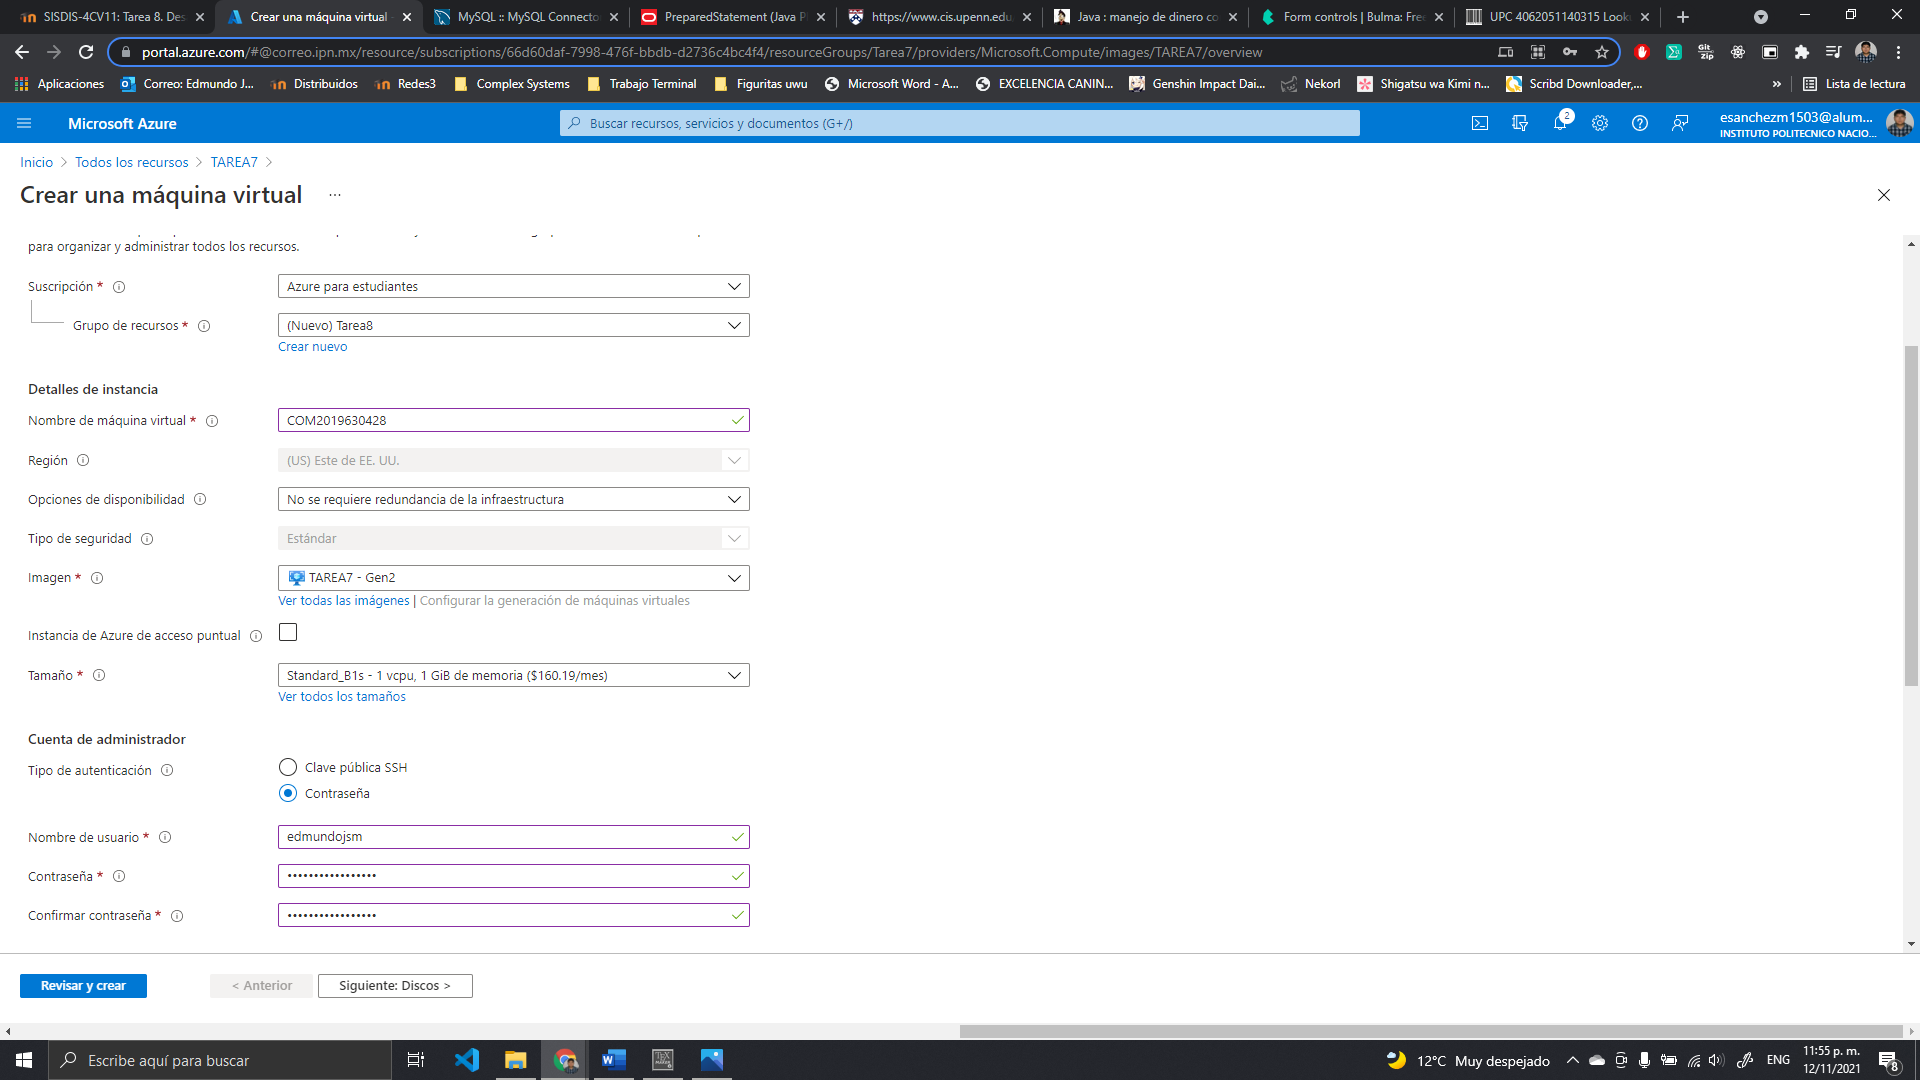
\includegraphics[scale=0.34]{resources/Infobasica.png}
			\caption{Datos básicos de la maquina virtual.}\label{fig:picture}
		\end{figure}
		\begin{figure}[H]
			\centering
			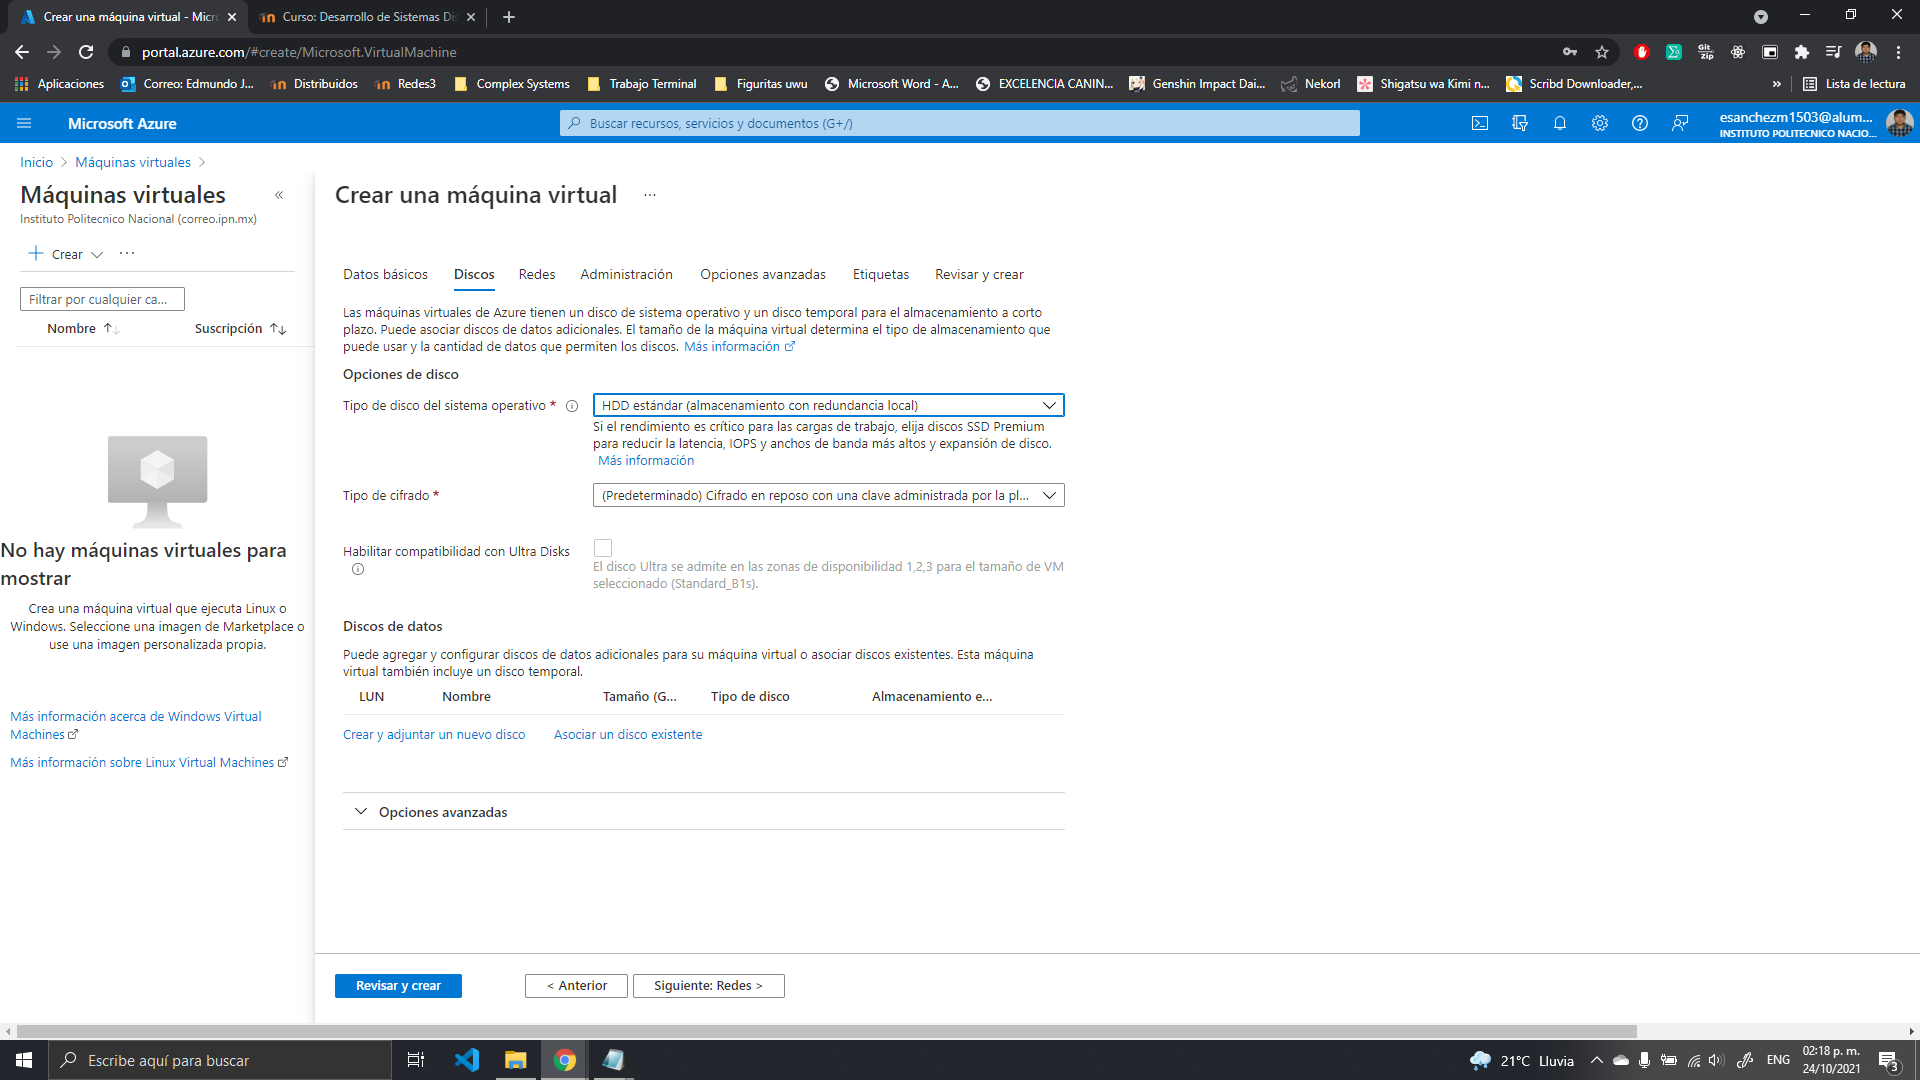
\includegraphics[scale=0.34]{resources/disco.png}
			\caption{Configuración del tipo de disco de la maquina virtual.}\label{fig:picture}
		\end{figure}
		\begin{figure}[H]
			\centering
			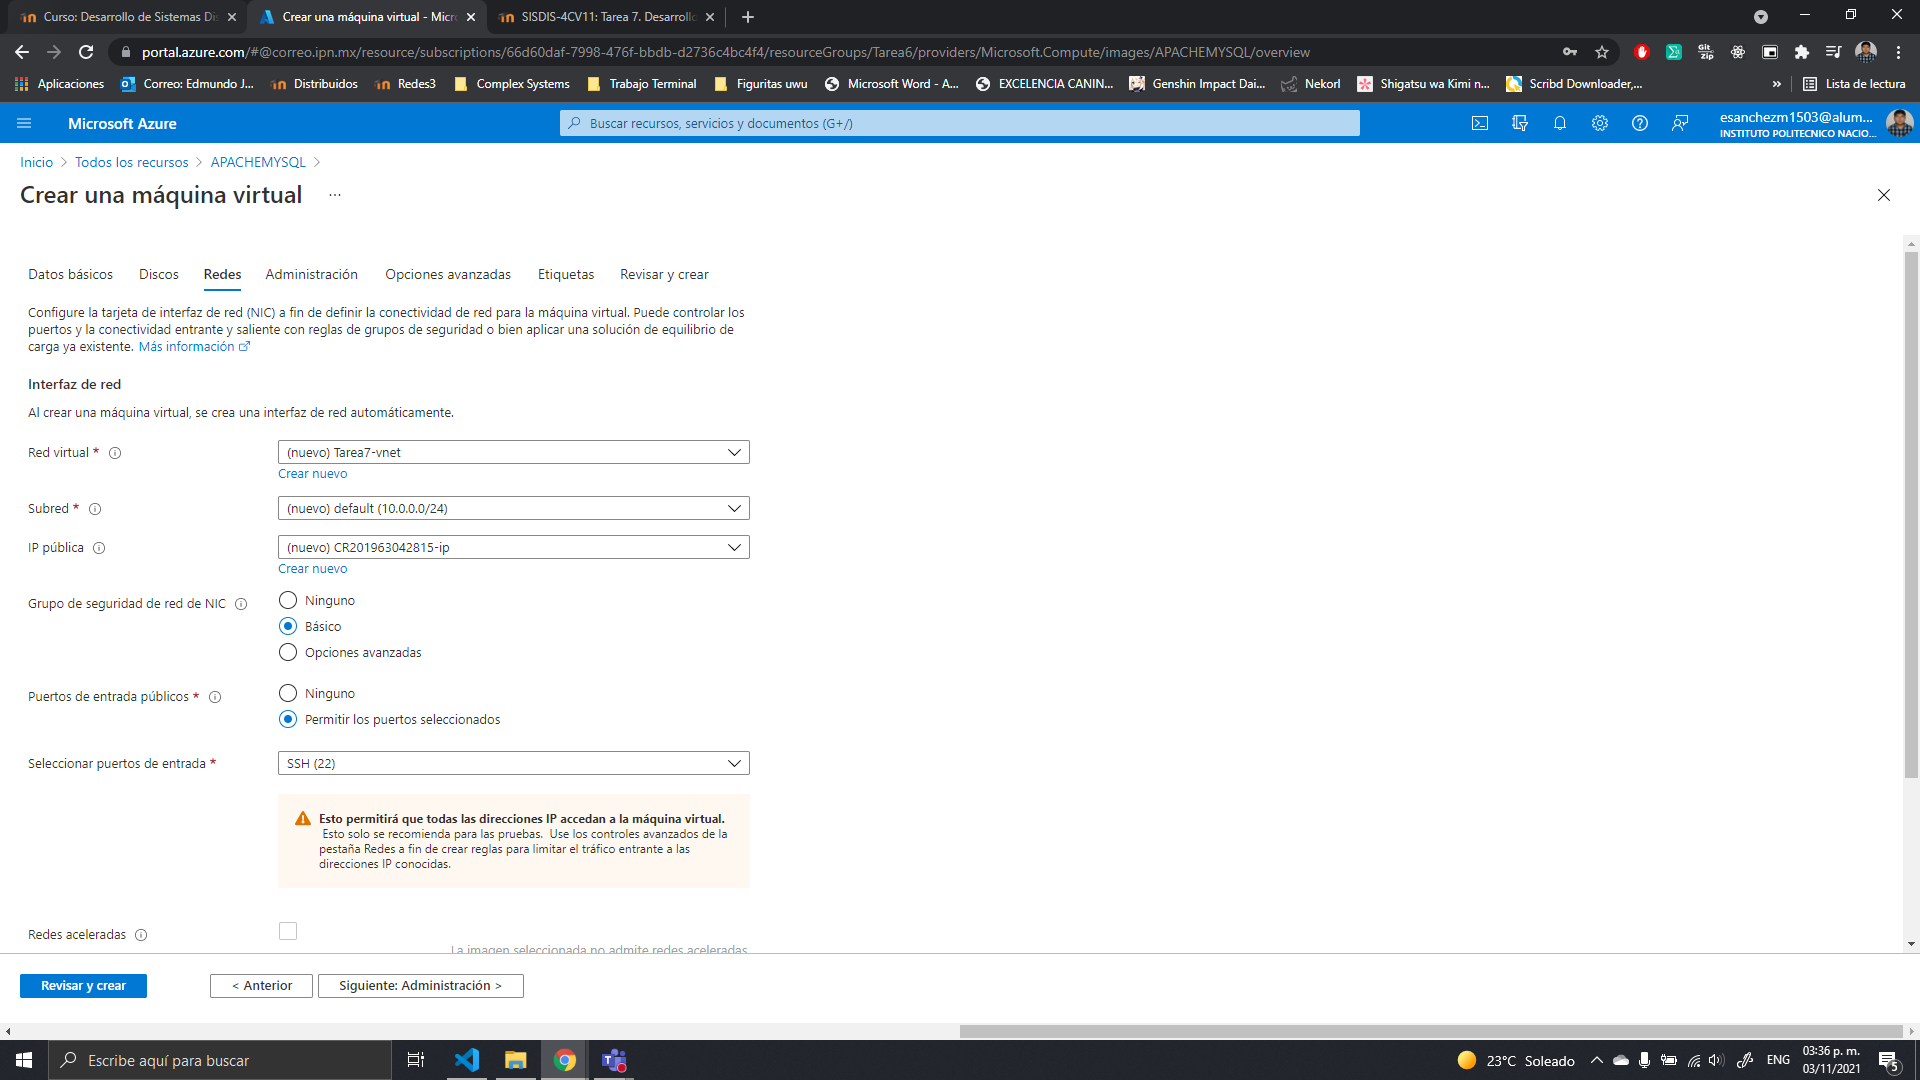
\includegraphics[scale=0.34]{resources/redes.png}
			\caption{Información sobre la redes de la maquina virtual.}\label{fig:picture}
		\end{figure}
		\begin{figure}[H]
			\centering
			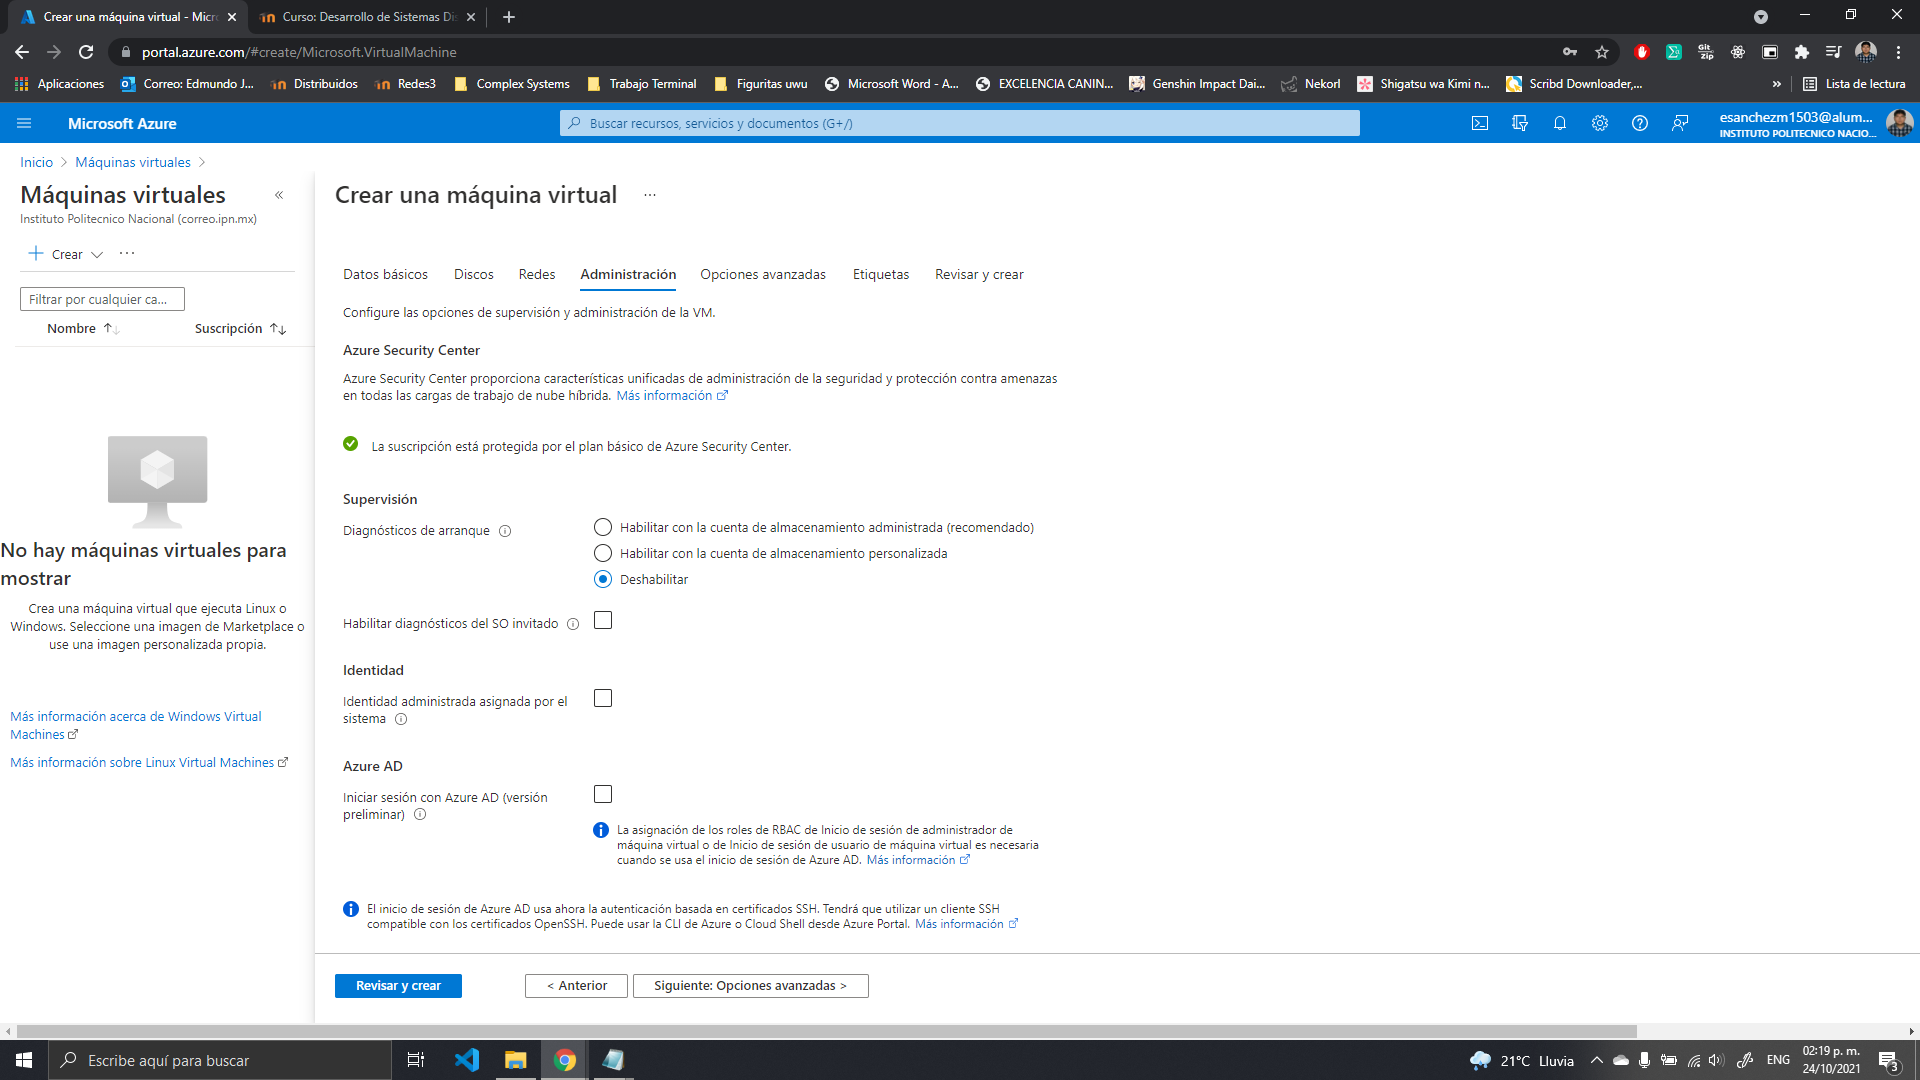
\includegraphics[scale=0.34]{resources/admin.png}
			\caption{Configuración de la administración de la maquina virtual.}\label{fig:picture}
		\end{figure}
		\begin{figure}[H]
			\centering
			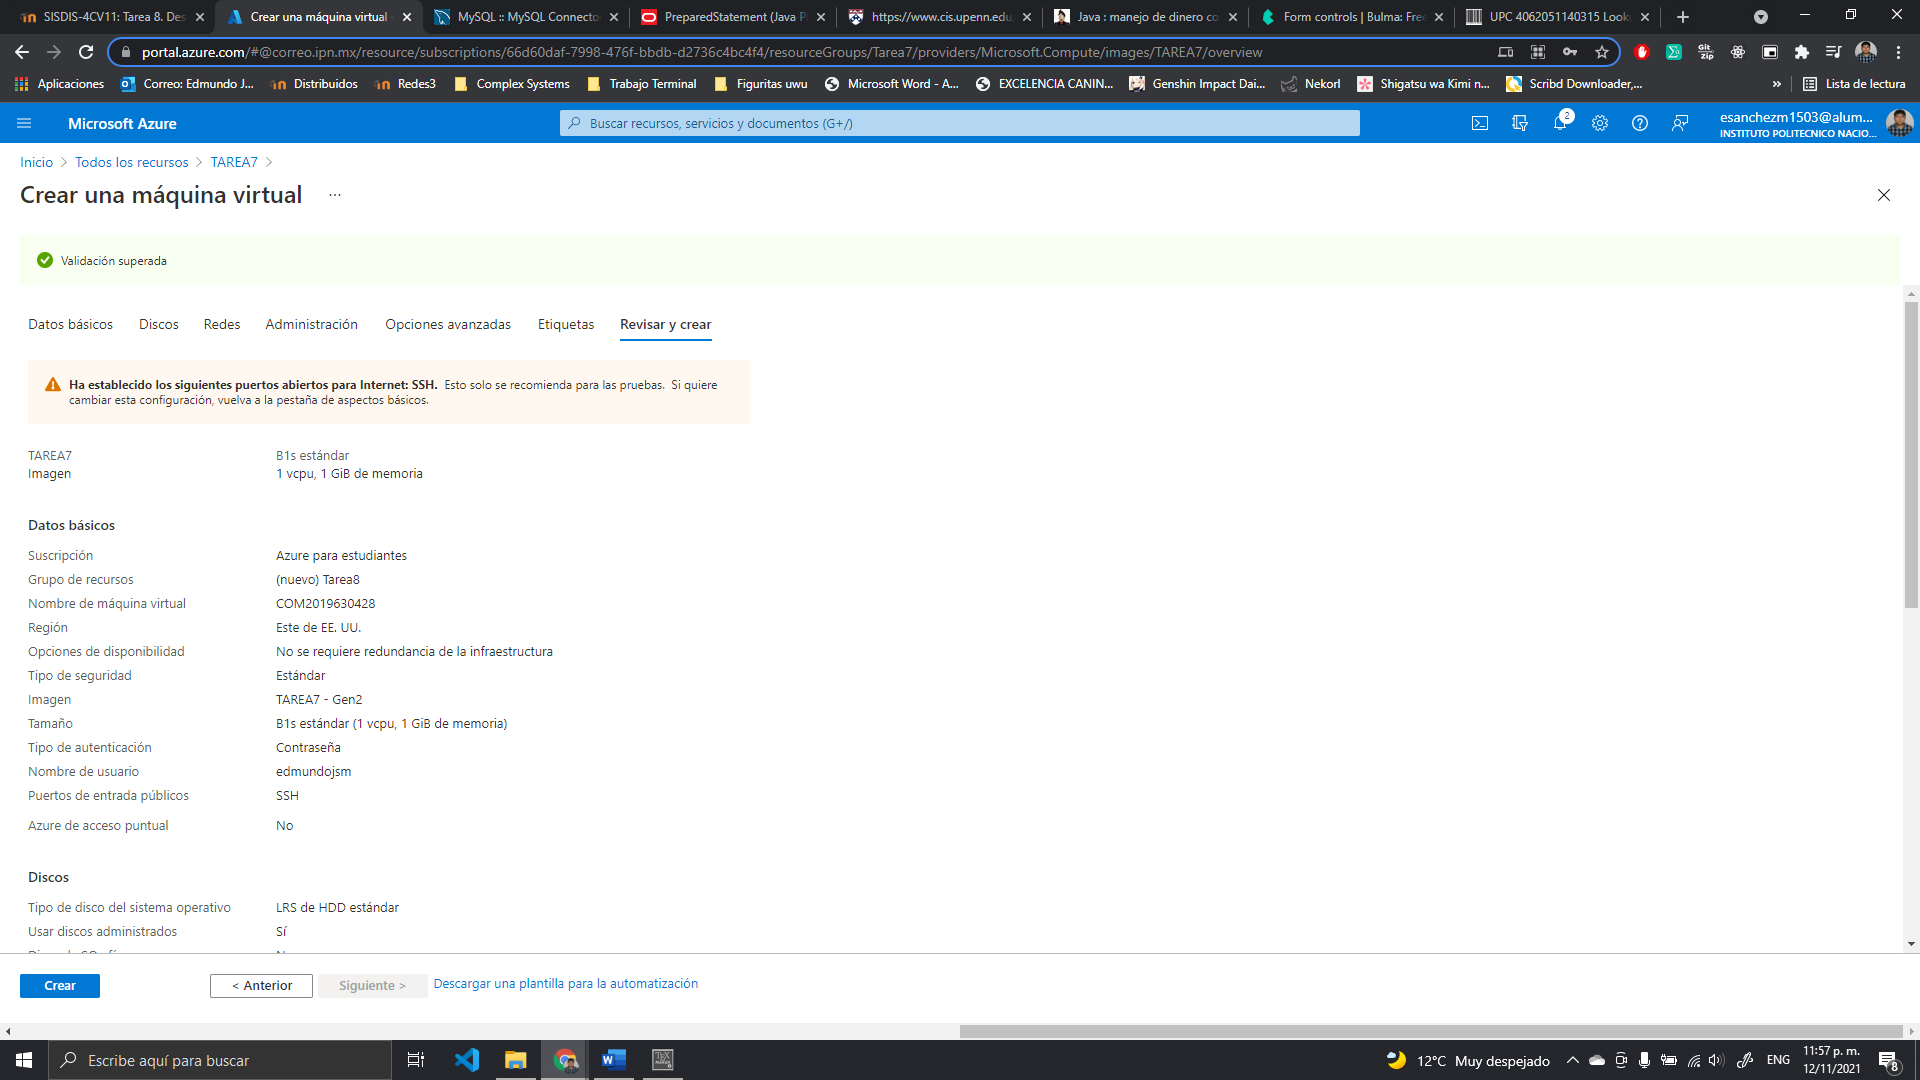
\includegraphics[scale=0.34]{resources/revisarycrear.png}
			\caption{Creación de la maquina virtual.}\label{fig:picture}
		\end{figure}
		\begin{figure}[H]
			\centering
			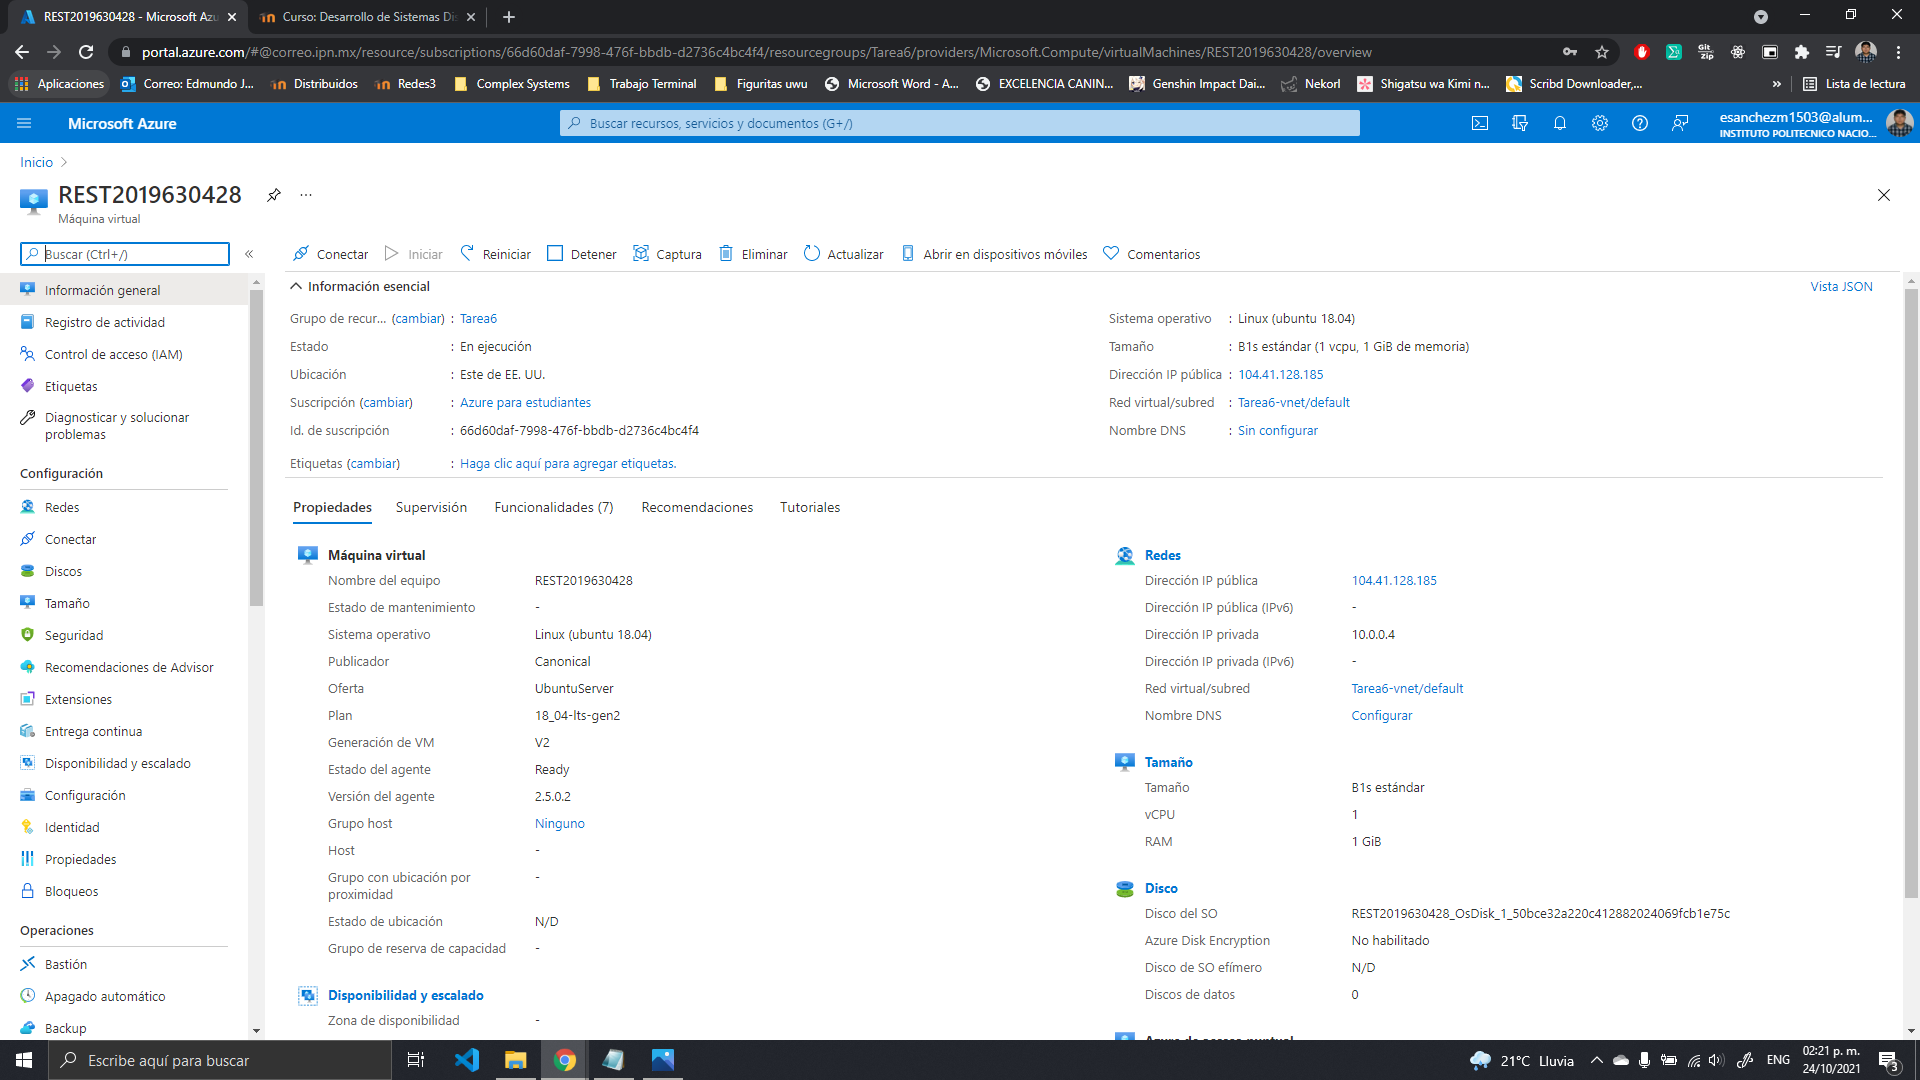
\includegraphics[scale=0.34]{resources/paneldecontrol.png}
			\caption{Panel de control de la maquina virtual.}\label{fig:picture}
		\end{figure}
		Una vez creada la maquina virtual tenemos que abrir el puerto 8080, ya que este puerto es el que ocupa Apache Tomcat, así podemos conectarnos de manera remota desde cualquier dispositivo , también es importante mencionar que si no se configura de manera correcta el puerto 8080 la conexión con la maquina virtual para poder visualizar el servicio web. En las figuras 7 y 8 podemos ver la configuración del puerto.
		\begin{figure}[H]
			\centering
			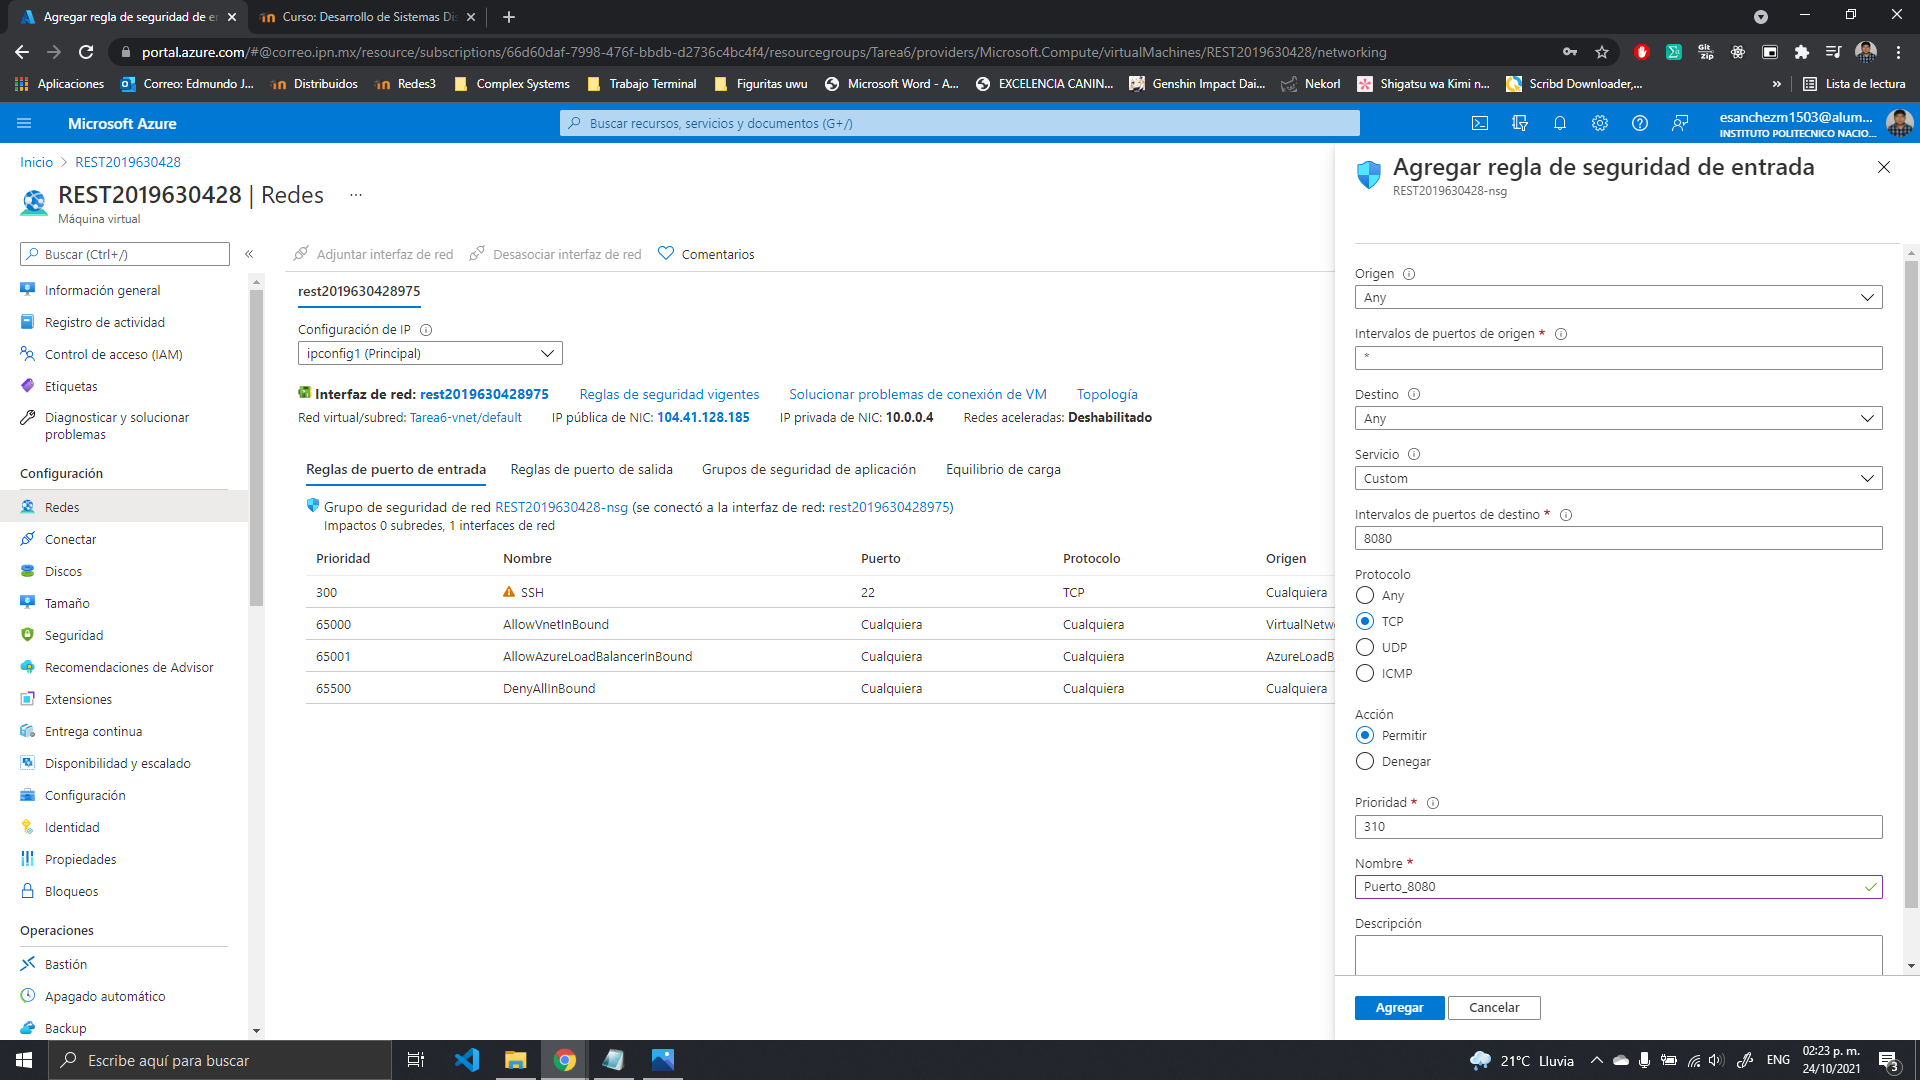
\includegraphics[scale=0.34]{resources/open8080.png}
			\caption{Configuración del puerto 8080.}\label{fig:picture}
		\end{figure}
		\begin{figure}[H]
			\centering
			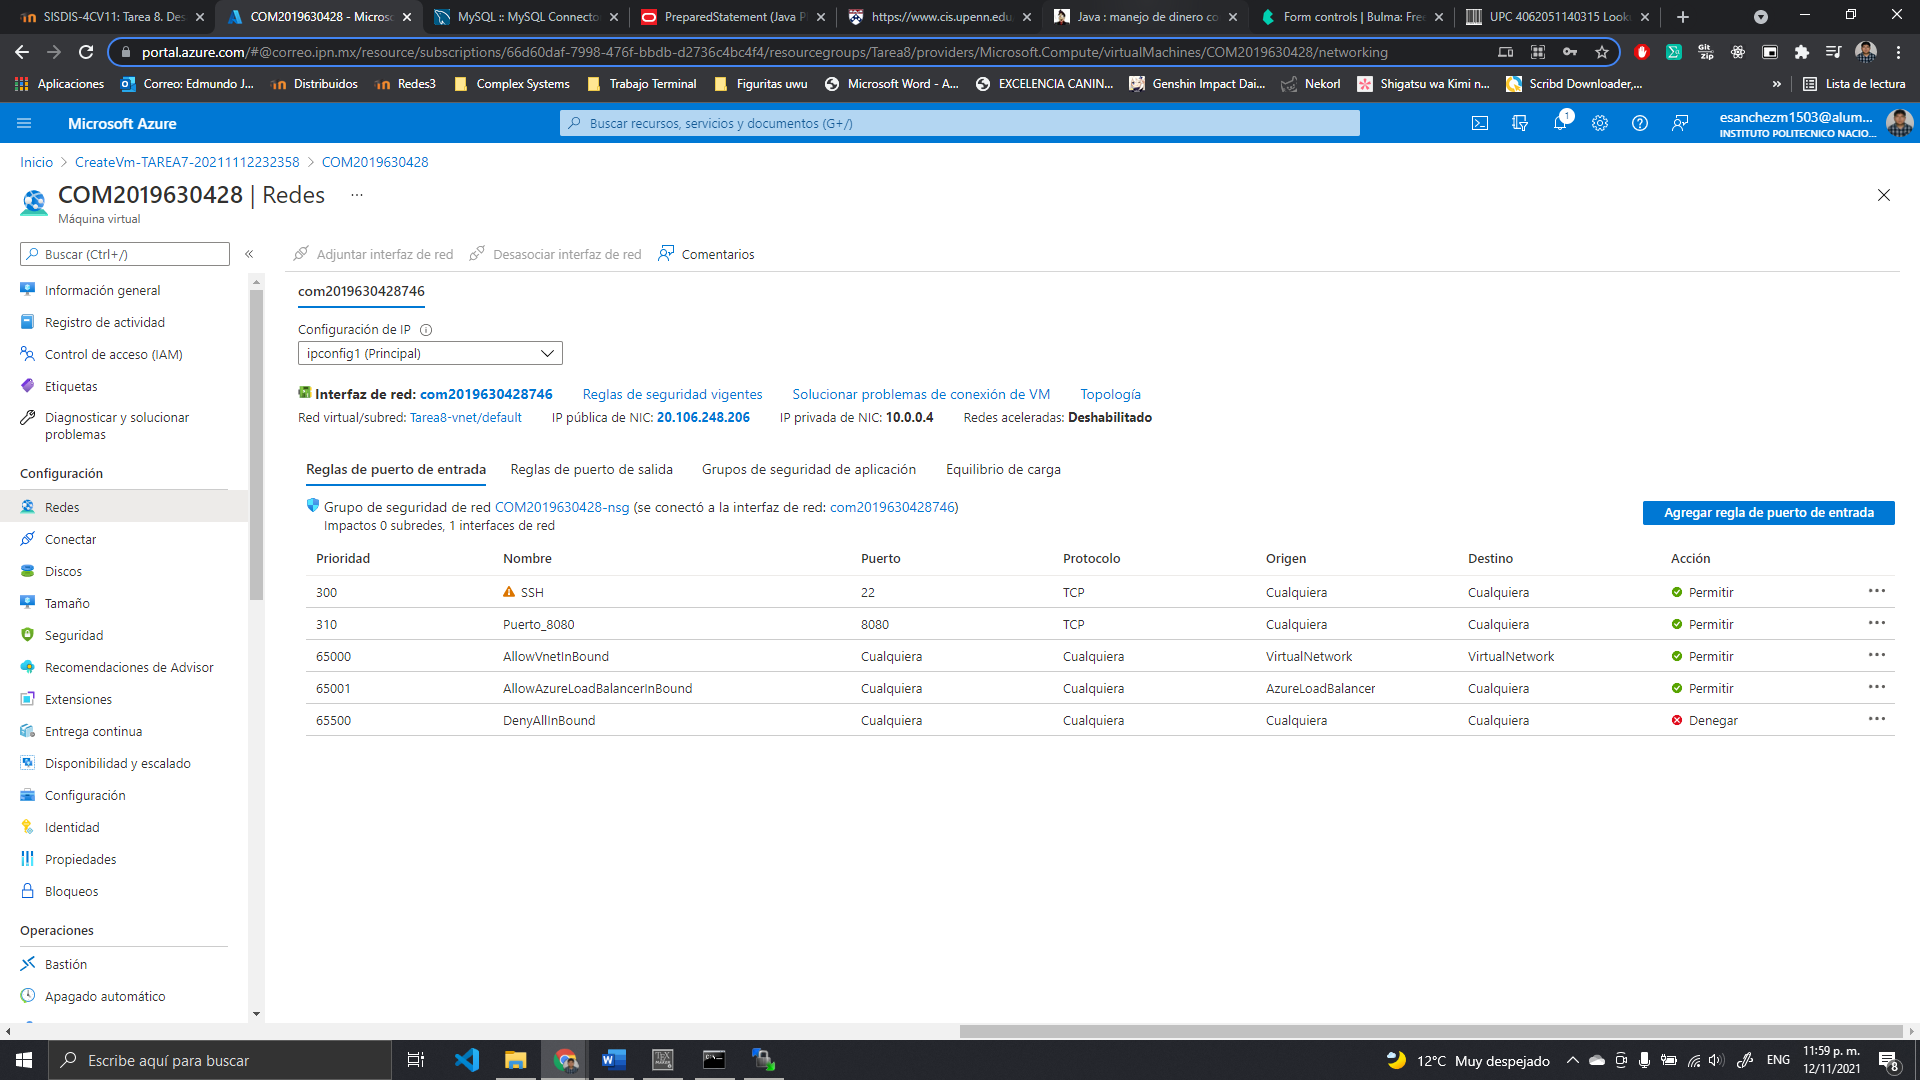
\includegraphics[scale=0.34]{resources/puertook.png}
			\caption{Puerto 8080 abierto correctamente.}\label{fig:picture}
		\end{figure}
		Ya teniendo la maquina preparada, procederemos a compilar nuestra aplicación estilo REST la cual fue desarrollada en Java, y a colocar los archivos HTML, JavaScript e imagen que usaremos como parte del front-end de la aplicación, pero antes de ellos veamos la preparación del entorno para ejecutar el sistema así como la creación de la base de datos a usar y la explicación del porque se añaden mas campos que los solicitados en la tarea.
		\subsection{Preparación del entorno y creación de la base de datos}		
	Para empezar debemos conectarnos a la maquina virtual vía SSH como podemos ver en la figura 9.
	\begin{figure}[H]
			\centering
			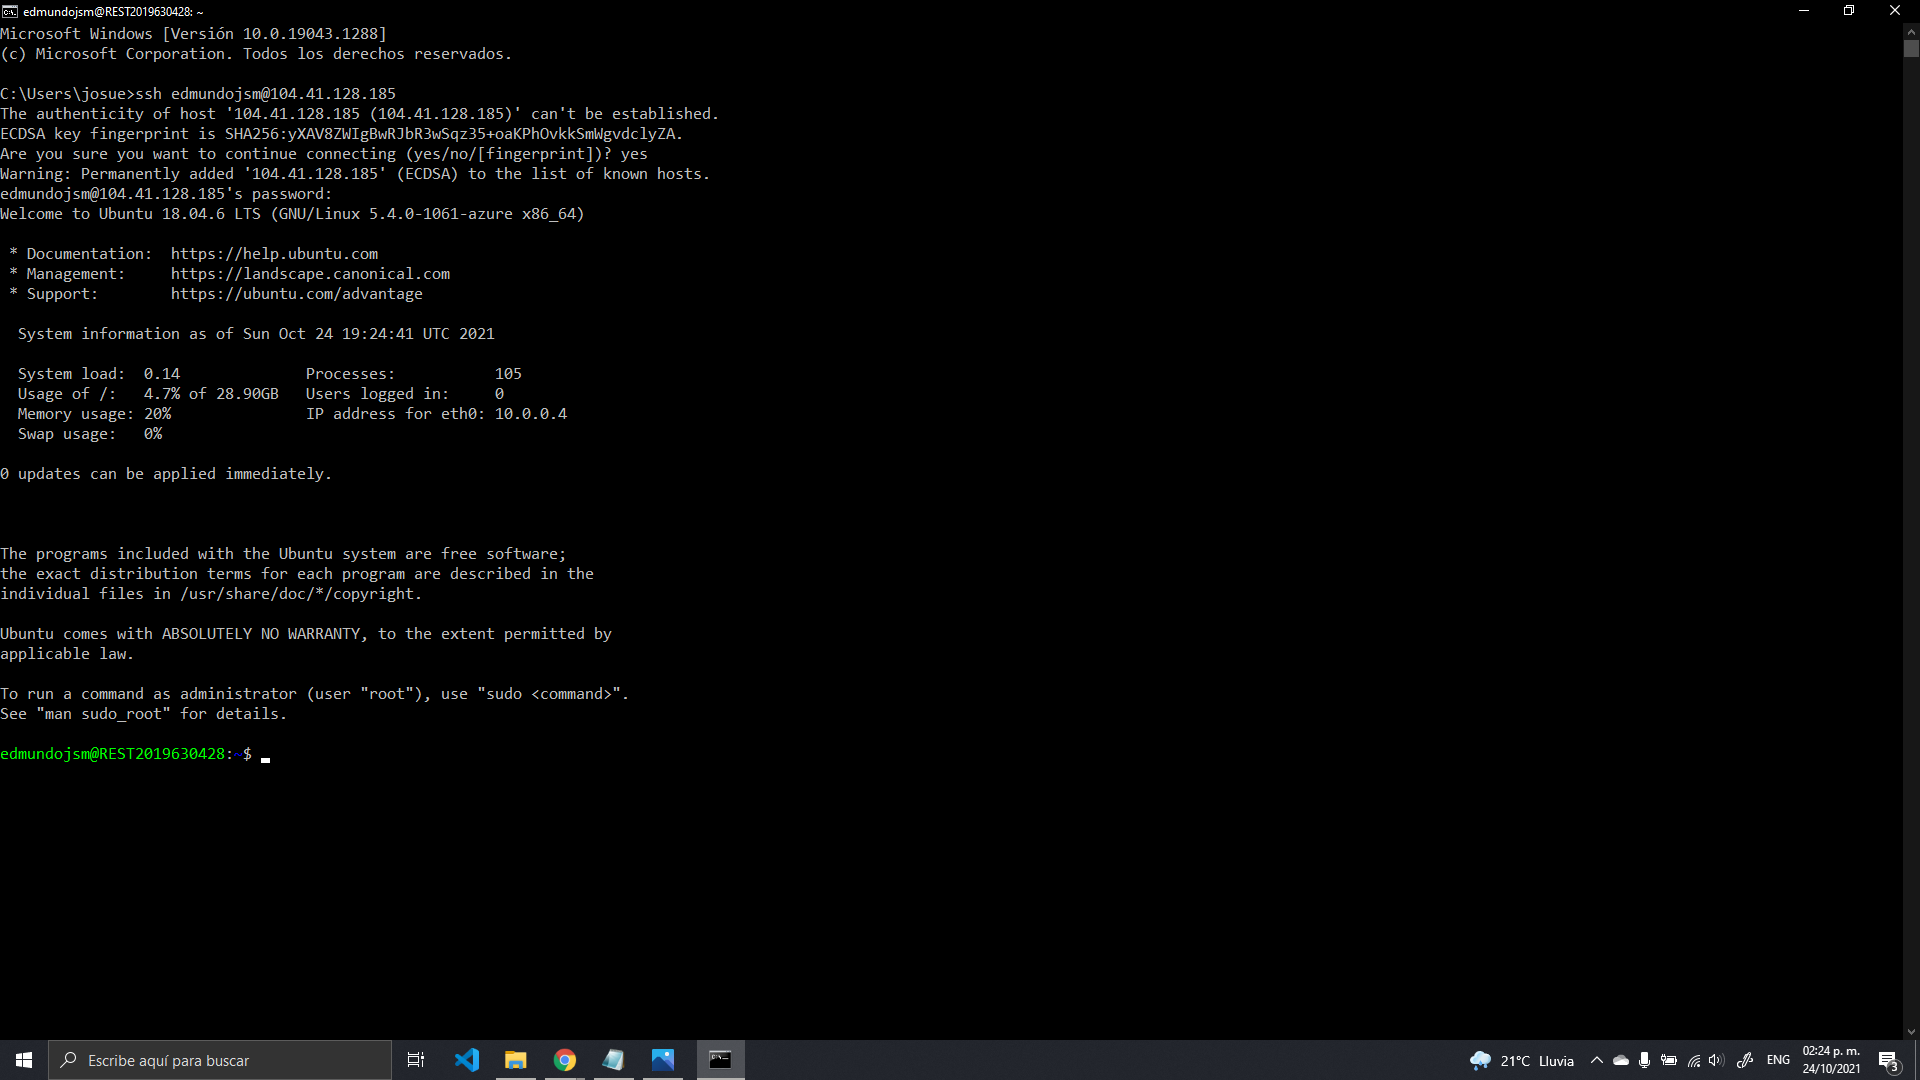
\includegraphics[scale=0.34]{resources/conexionssh.png}
			\caption{Conexión SSH con la maquina virtual.}\label{fig:picture}
		\end{figure}
		Ahora necesitaremos crear nuestra variables de entorno de CATLINA\_HOME y JAVA\_HOME así como hacer que Tomcat empiece a funcionar, como lo vemos en la figura 10.
		\begin{figure}[H]
			\centering
			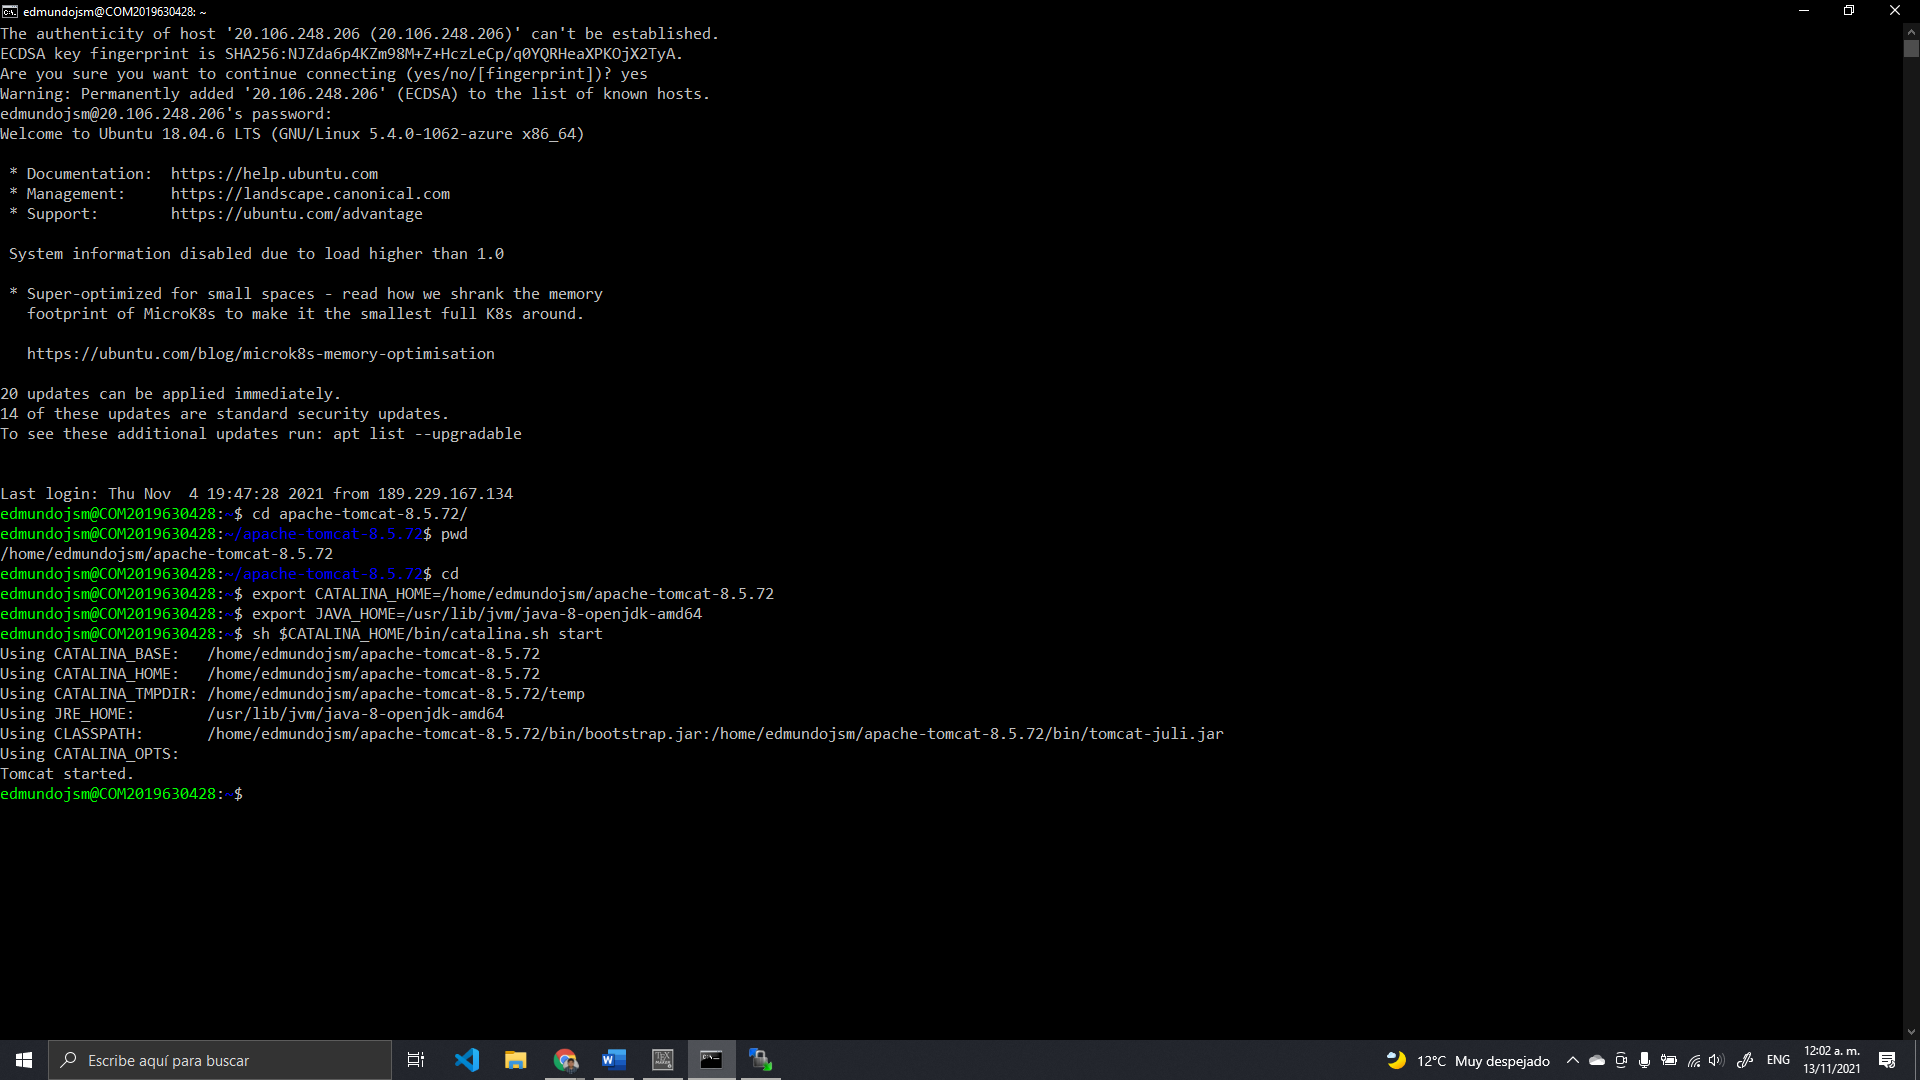
\includegraphics[scale=0.34]{resources/tomcat_variables_entorno.png}
			\caption{Variables de entorno asignadas y Tomcat corriendo.}\label{fig:picture}
		\end{figure}
		Finalmente nos toca crear la base de datos a usar la cual esta basada con los requerimientos funcionales de la tarea, sin embargo, se añadieron dos campos mas los cuales considero importantes para un tipo de sistema como el que se esta desarrollando, estos campos son nombre de tipo varchar y UPC de tipo bigint, este ultimo es conocido como CÓDIGO UNIVERSAL DEL PRODUCTO, el cual es usado para poder rastrear los artículos comerciales en las tiendas, este UPC es el clásico código de barras que podemos encontrar en los artículos que compramos, esto nos podría permitir tener una mejor gestión en nuestro almacén tanto física como de manera virtual, esto claro, si se desea hacer aun mas grande esta aplicación, la razón del por cual es de tipo bigint es porque consta de 12 dígitos numéricos y bigint es el único tipo de dato que soporta la longitud de este dato, mencionar que por obvias razones un producto tiene un único UPC, mencionar que en las pruebas el UPC ingresado son números menores a 12 dígitos esto debido para facilitar la visualización de la información. Finalmente el script de la creación de tablas y de las llaves foráneas se anexan en un archivo de texto con el nombre de ``Base de datos''. Todo el proceso de creación lo podemos ver en las figuras 11 y 12.
		\begin{figure}[H]
			\centering
			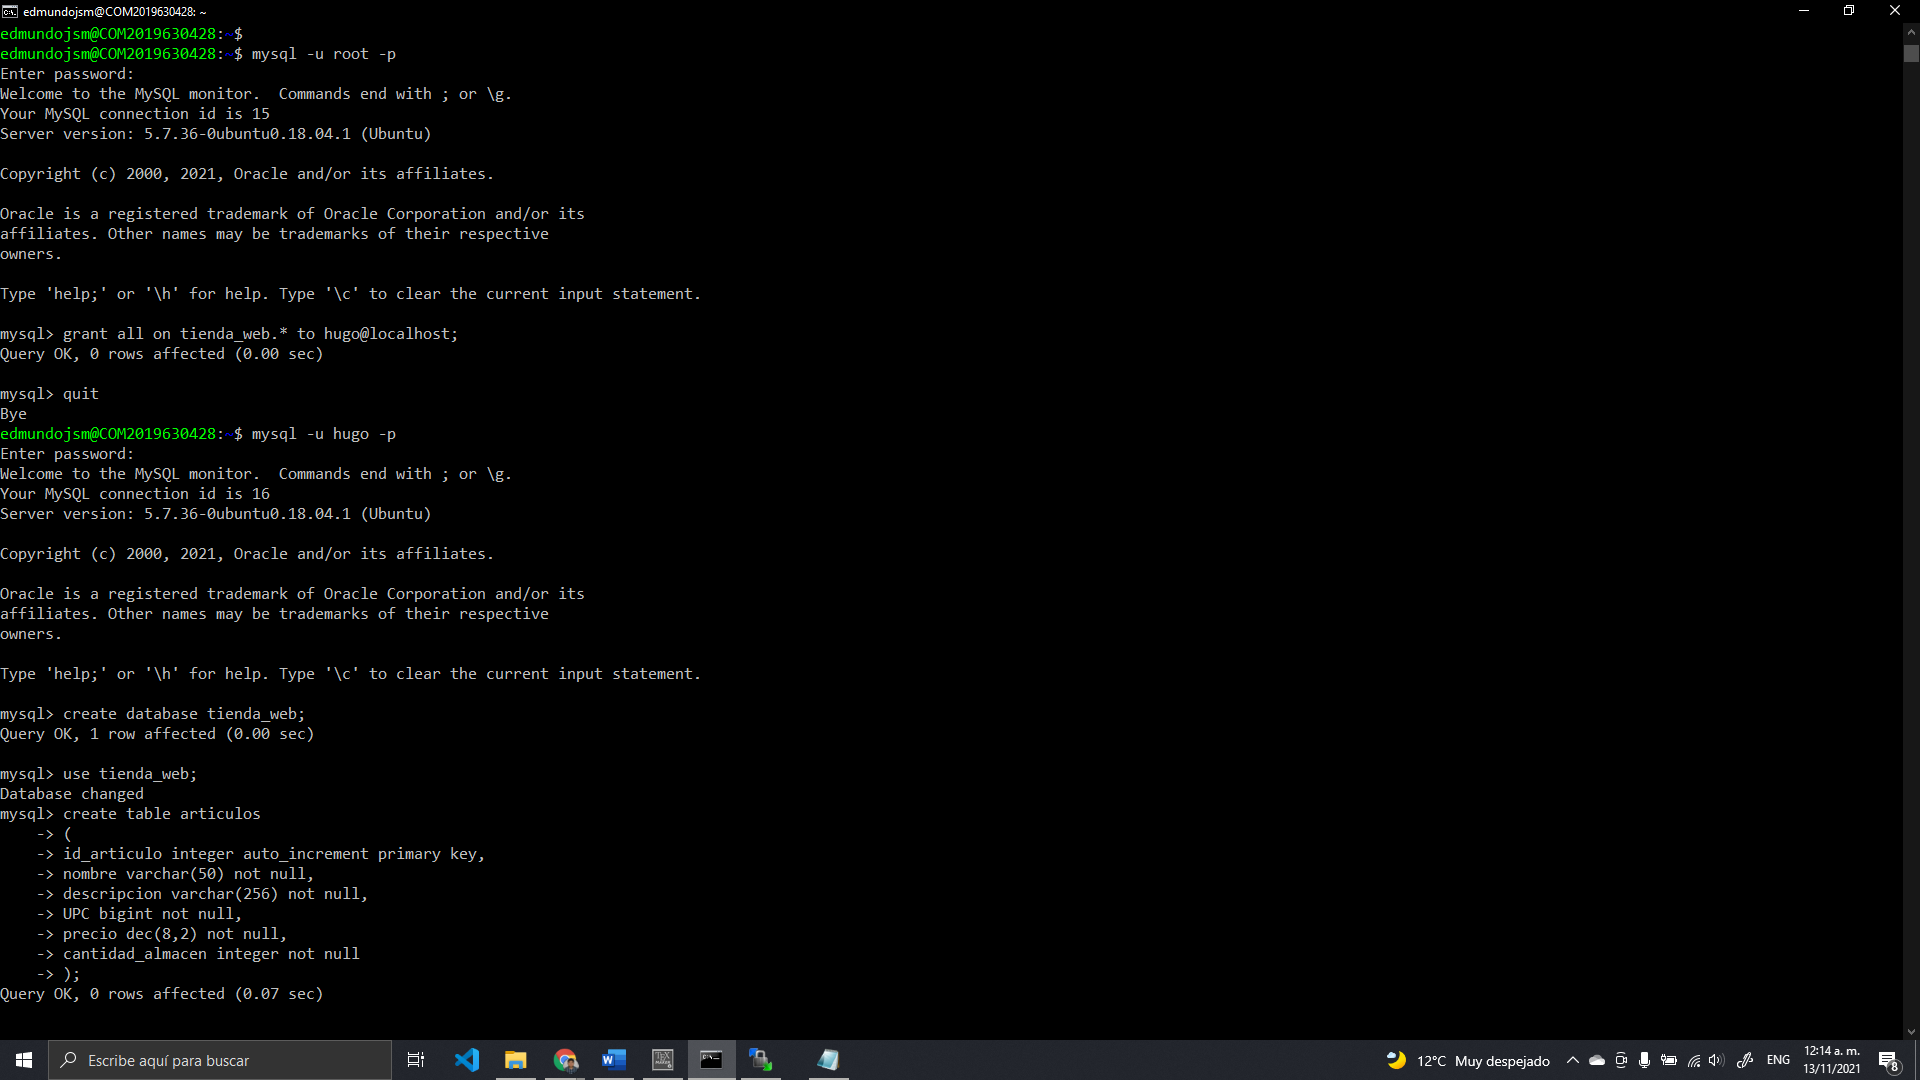
\includegraphics[scale=0.34]{resources/mysql1.png}
			\caption{Dando permisos al usuario hugo para la base de datos a usar y primera parte de la creación de esta.}\label{fig:picture}
		\end{figure}
		\begin{figure}[H]
			\centering
			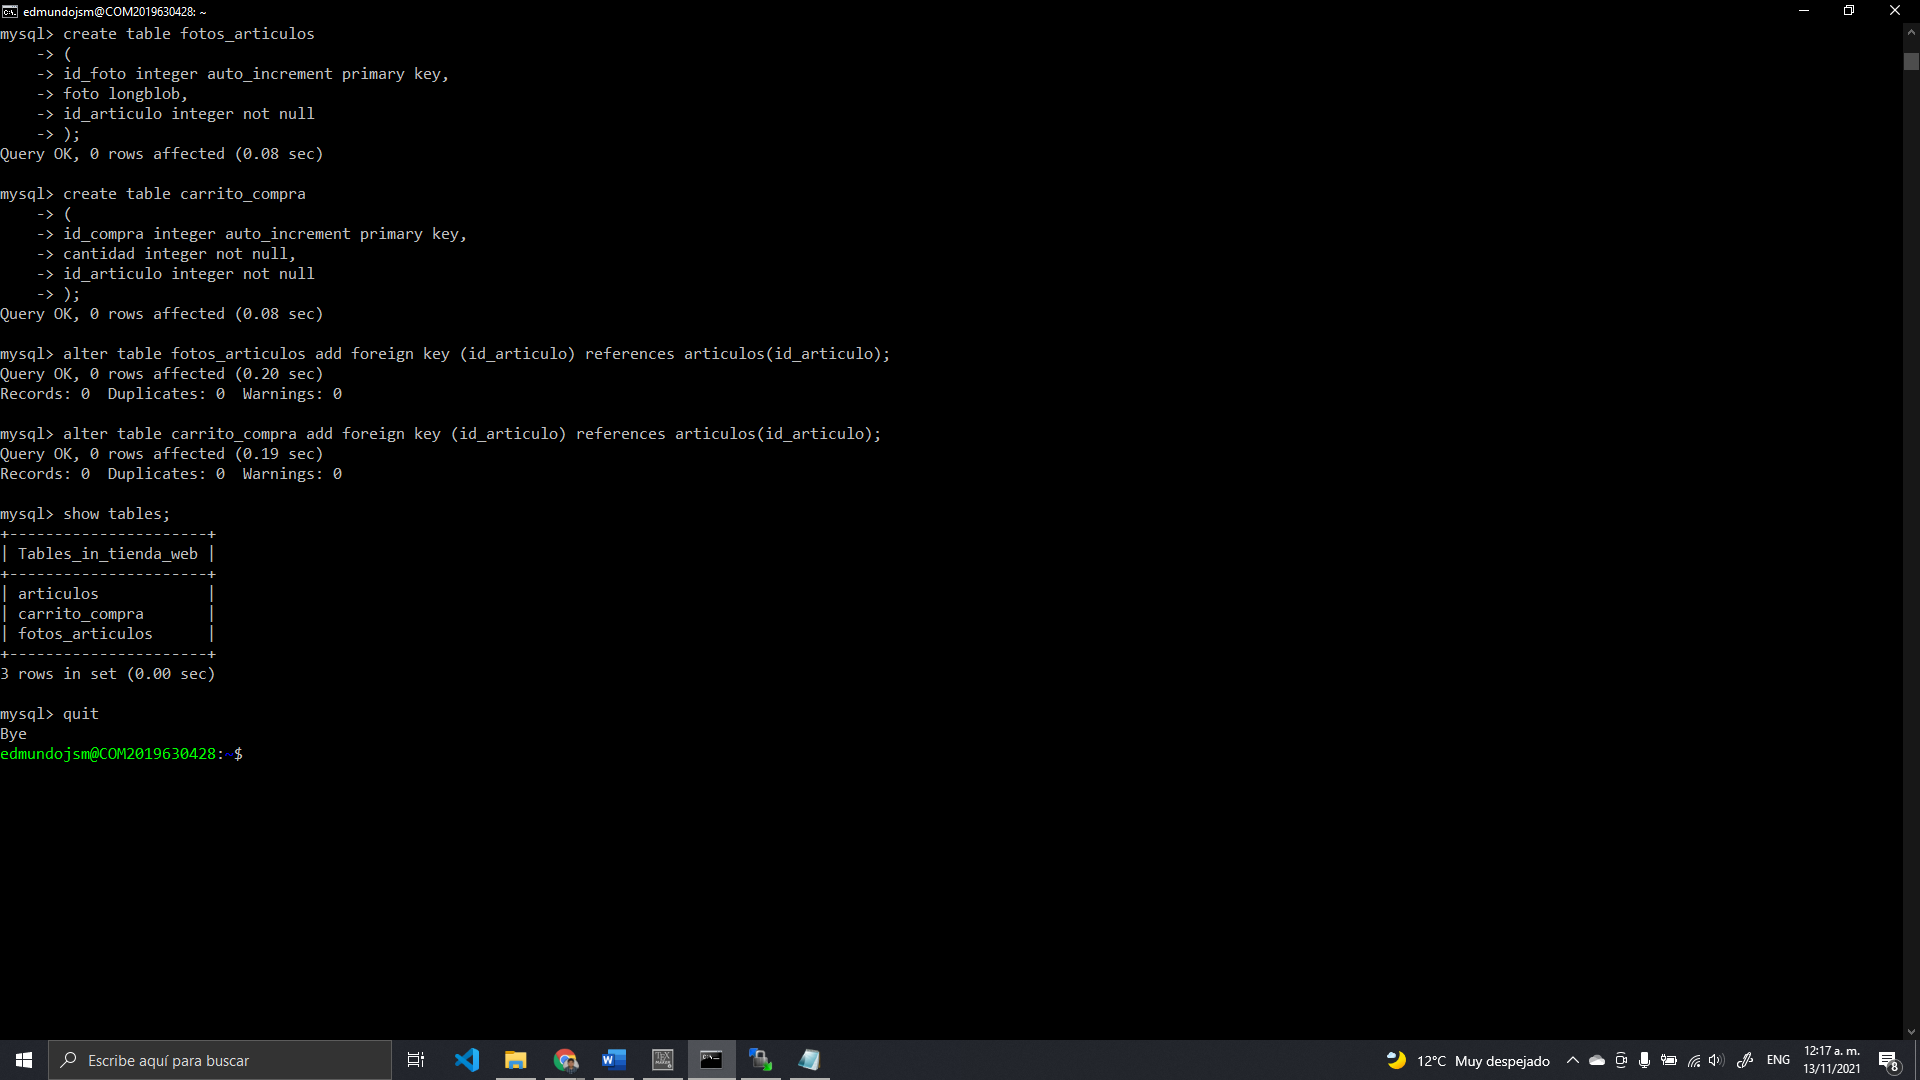
\includegraphics[scale=0.34]{resources/mysql2.png}
			\caption{Ultima parte de la creación de la base de datos.}\label{fig:picture}
		\end{figure}
		\subsection{Compilación del código para el back-end y colocación de archivos para el front-end en ROOT}
		Ahora tome como base el código de servicio, solo cambiamos la clase Usuario por una clase Articulo y modificar el archivo Servicio.java para cumplir con los requerimientos funcionales, mencionar también que como tal no hay compilación del código para el front-end ya que el front-end fue desarrollado con HTML-JS y este no necesita compilación pero si necesitamos tener los archivos en el servidor Tomcat en la carpeta ROOT. Ahora nos toca compilar el servicio, generar el .war y copiarlo a la carpeta webapps para poder tener el servicio en linea usando Tomcat, todo esto se ve en la figura 13 y 14, finalmente vemos los contenidos en la carpeta webapps y ROOT de nuestra carpeta de Tomcat, esto también lo podemos ver en la figura 14.
		\begin{figure}[H]
			\centering
			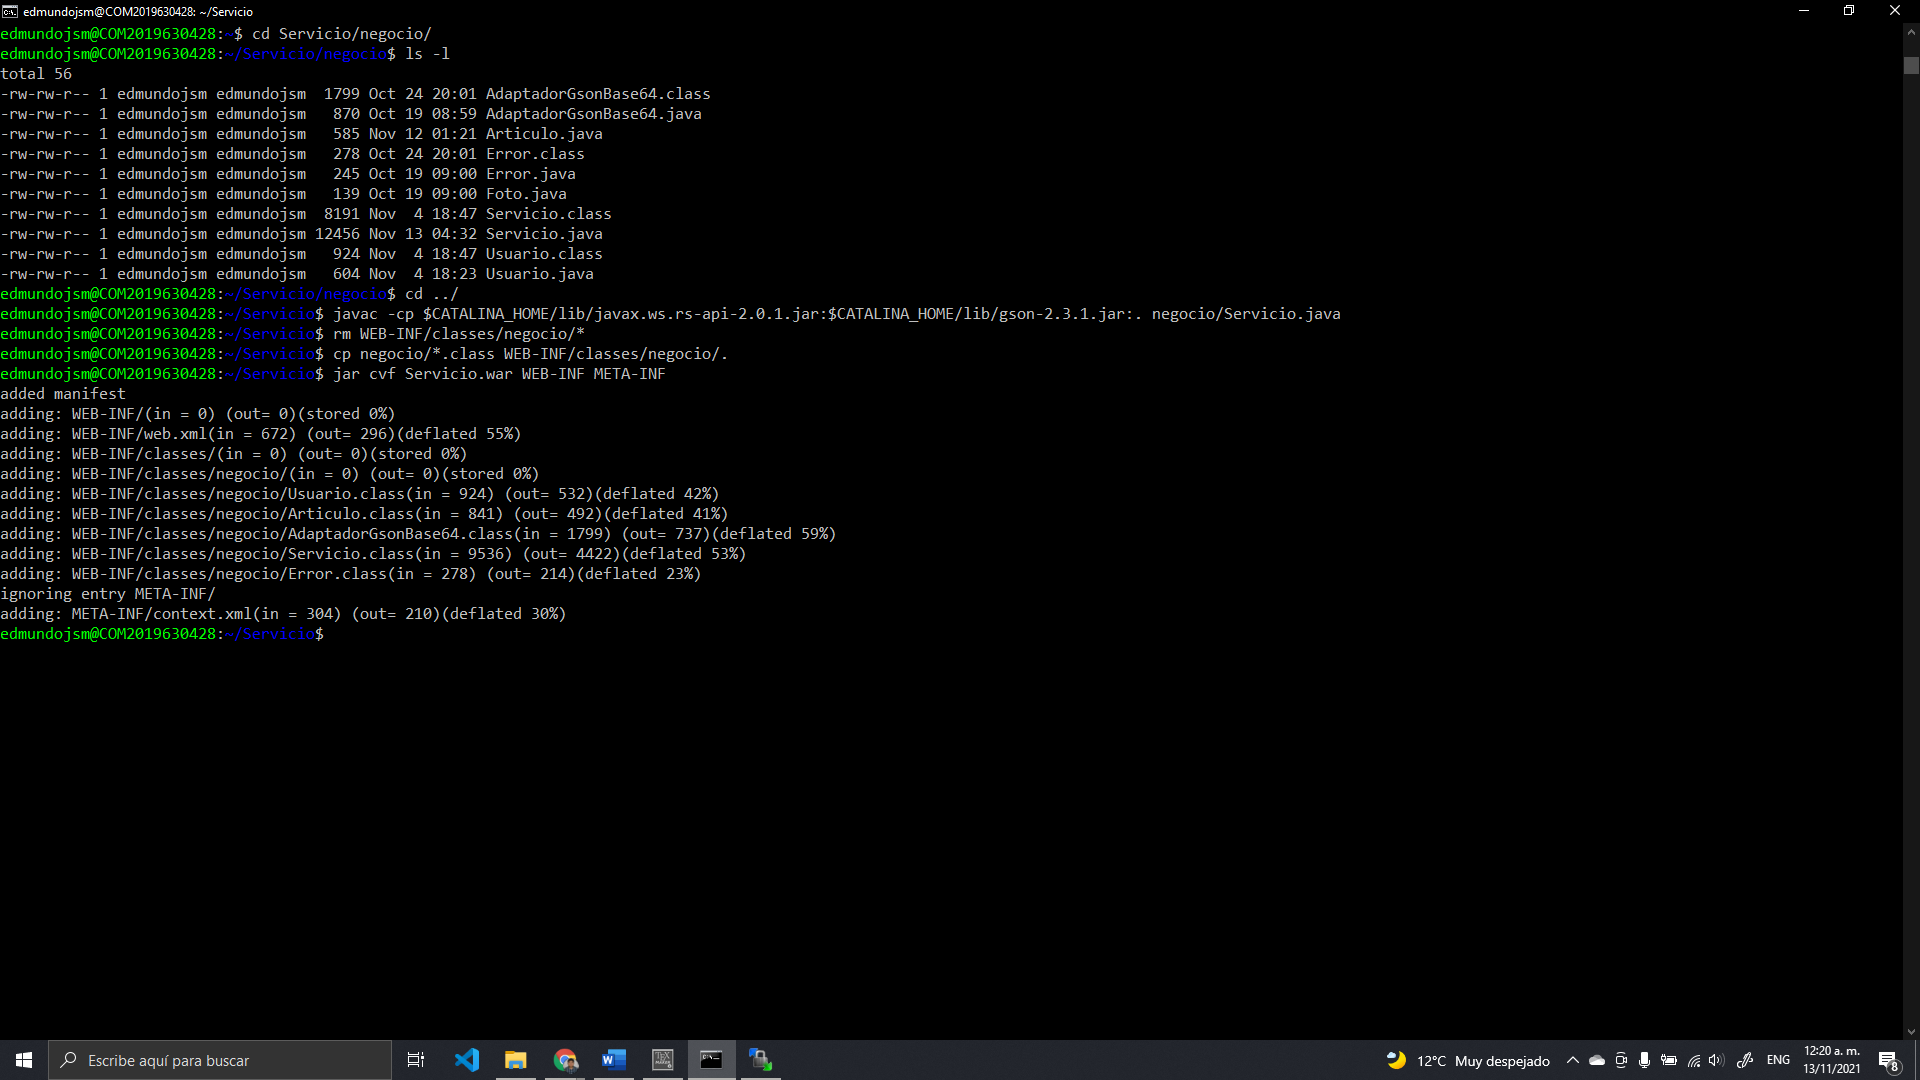
\includegraphics[scale=0.34]{resources/compilacionback.png}
			\caption{Compilación de Servicio.}\label{fig:picture}
		\end{figure}
		\begin{figure}[H]
			\centering
			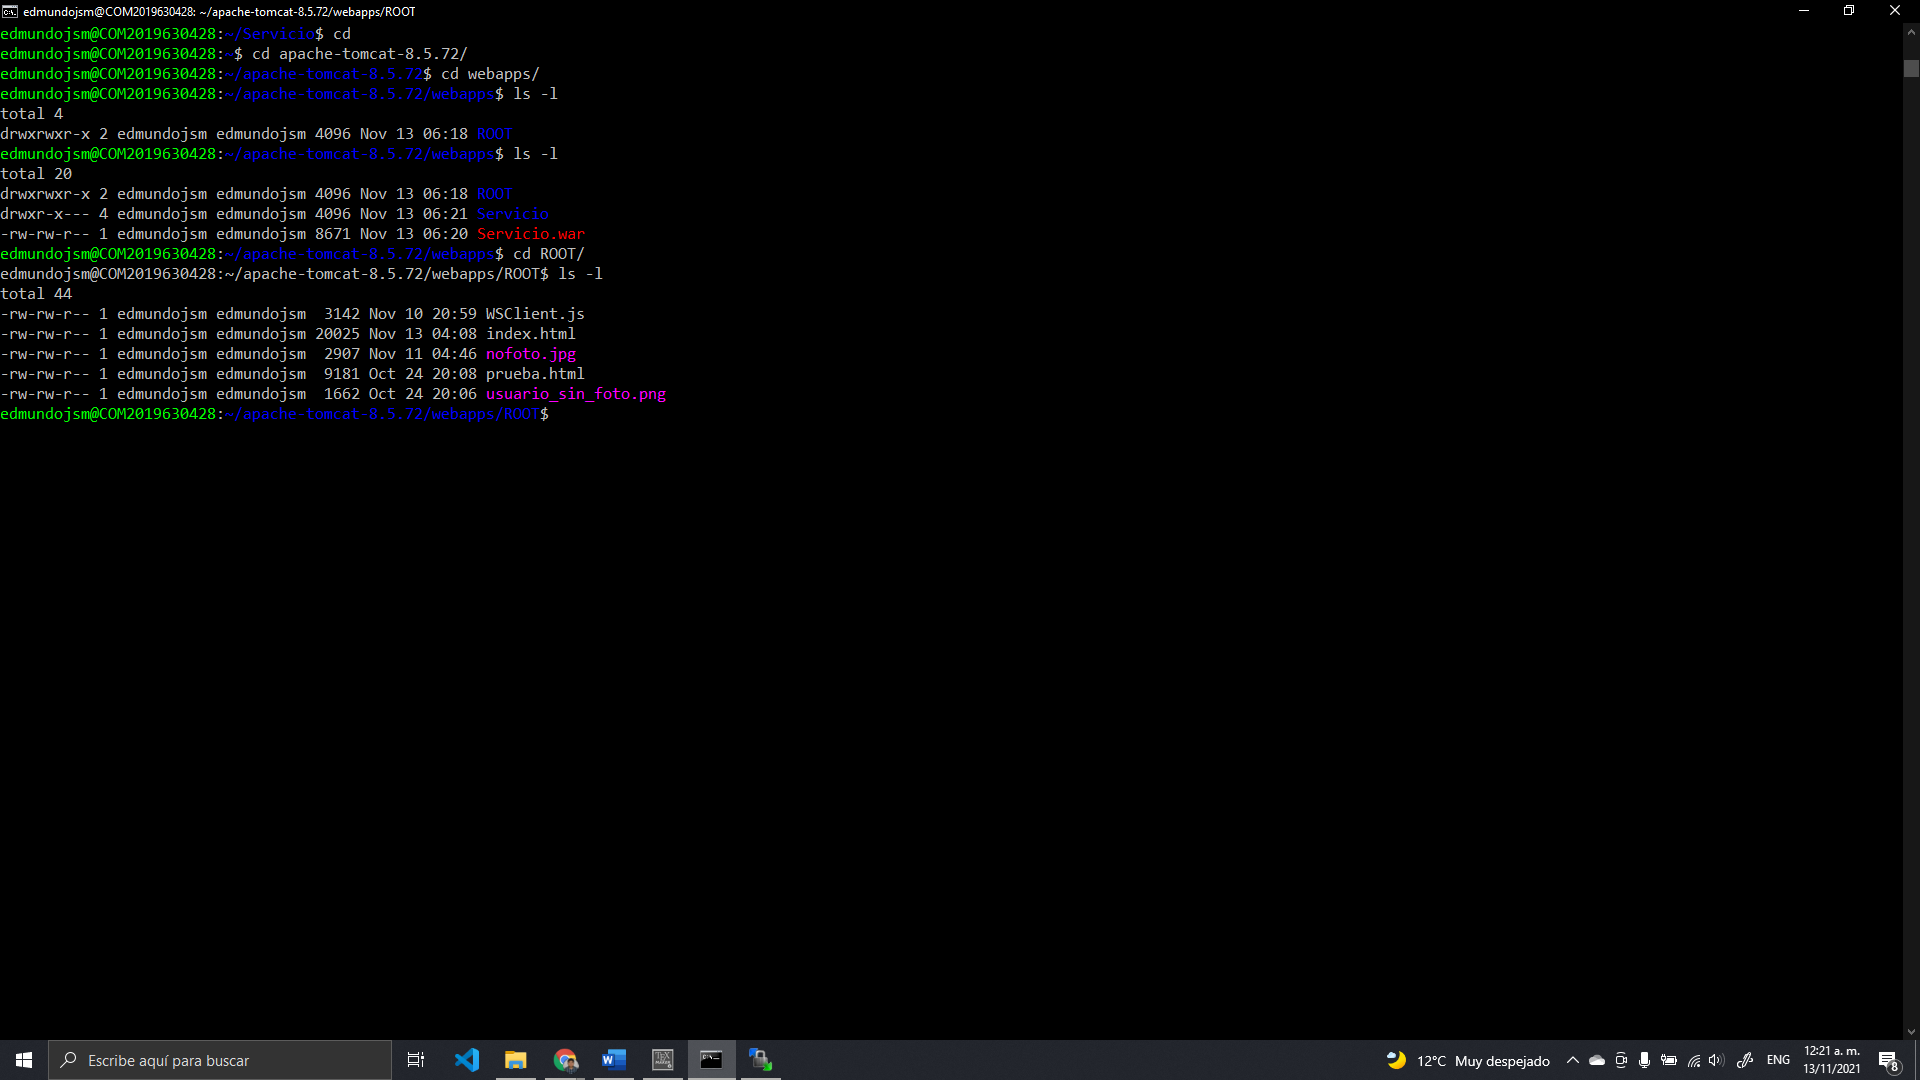
\includegraphics[scale=0.34]{resources/warinwebappsandfront.png}
			\caption{Contenidos de la carpeta webapps y ROOT de Tomcat.}\label{fig:picture}
		\end{figure}
	\section{Pruebas}
	Es importante mencionar que para el desarrollo de esta practica se usaron dos frameworks uno es Bulma el cual es un framework de CSS y SweetAlert2 el cual es un framework para alertas de JavaScript. Ahora pasemos a las pruebas del sistema desarrollado, mencionar que las pruebas se desarrollaron tanto en mi computadora personal como en mi celular para cumplir con uno de los requerimientos no funcionales y estas están vinculadas entre si.
		\subsection{Prueba 1. Captura de articulo}
	En los requerimientos funcionales nos solicitan mostrar 2 un menú con las opciones de Captura de articulo y Compra de artículos, sin embargo, decidí agregar dos mas, la opción de Inicio la cual nos mostrara los todos los artículos que se hayan registrados y en el caso de no tener ninguno nos dirá que no hay artículos y el de Carrito de compra el cual es solicitado que se nos presente al ver la opción de Compra de artículos, pero considere mas cómodo que se viera en todo momento para el usuario ya que considero que es mas amigable, esto lo podemos ver en la figura 15.
		\begin{figure}[H]
			\centering
			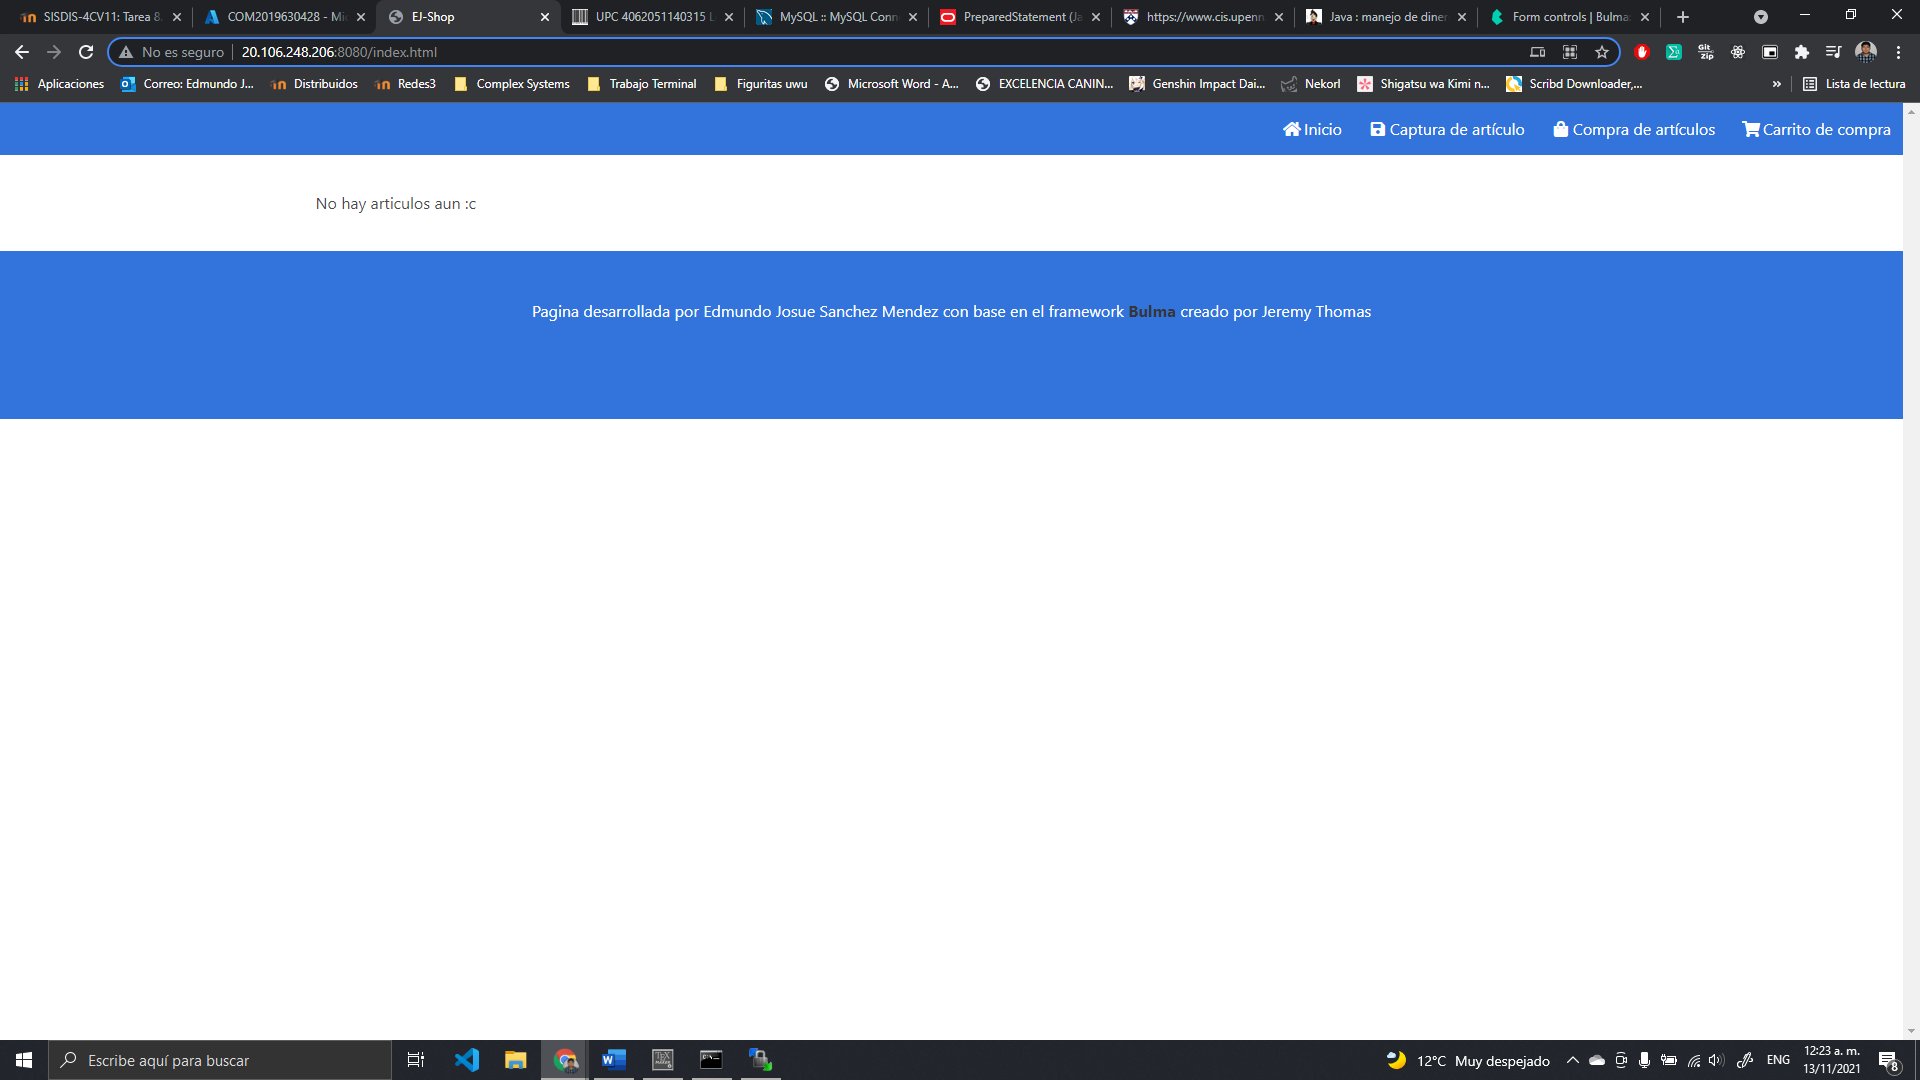
\includegraphics[scale=0.34]{resources/serviciofuncionando.png}
			\caption{Pagina de inicio sin artículos registrados.}\label{fig:picture}
		\end{figure}
	En la figura 16 podemos ver la captura de un articulo con toda la información que necesitamos guardar en la base de datos, esta prueba contiene una foto para al articulo, al darle click al botón de Guardar articulo y esperar pocos segundos nos sale la alerta que podemos ver en la figura 17, la cual indica como el articulo fue dado de alta correctamente y nos vacia el formulario incluyendo la imagen.
		\begin{figure}[H]
			\centering
			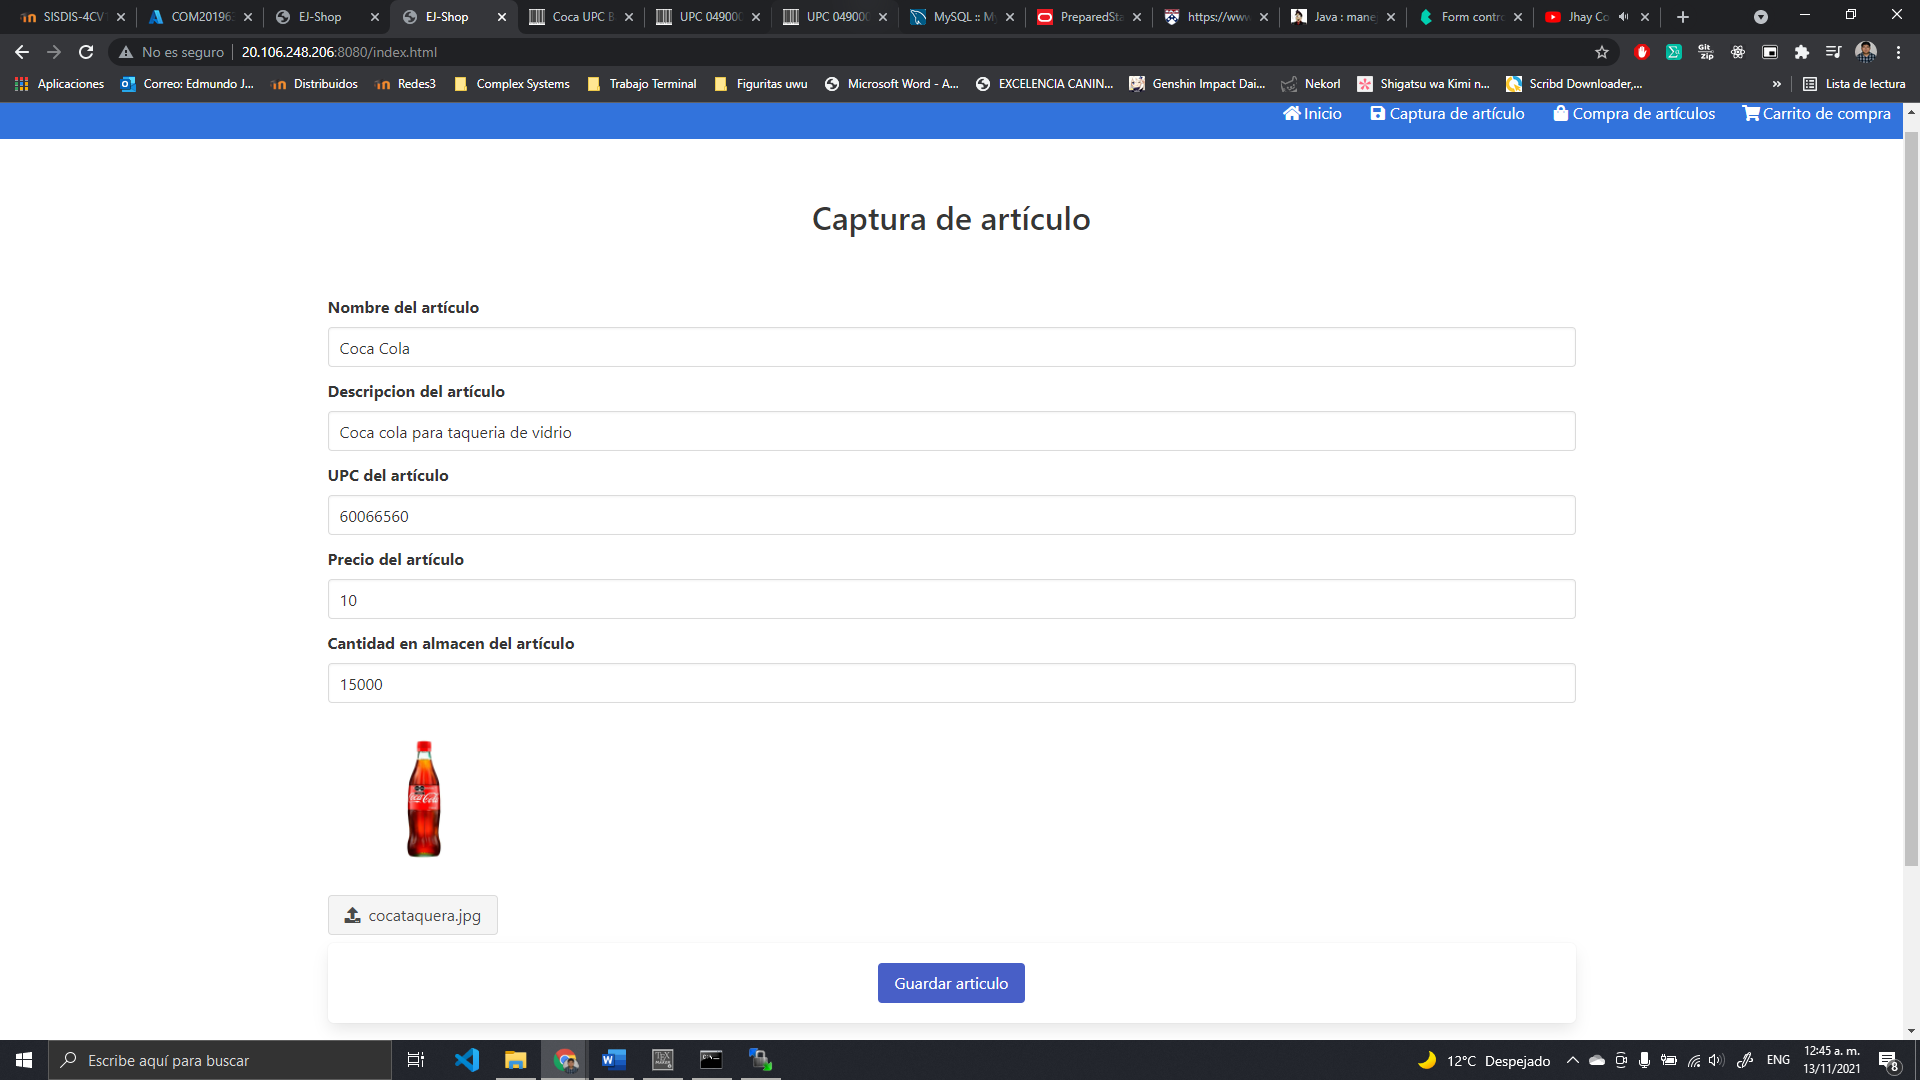
\includegraphics[scale=0.34]{resources/P1.png}
			\caption{Prueba 1.1. Articulo dado de alta con foto.}\label{fig:picture}
		\end{figure}
		\begin{figure}[H]
			\centering
			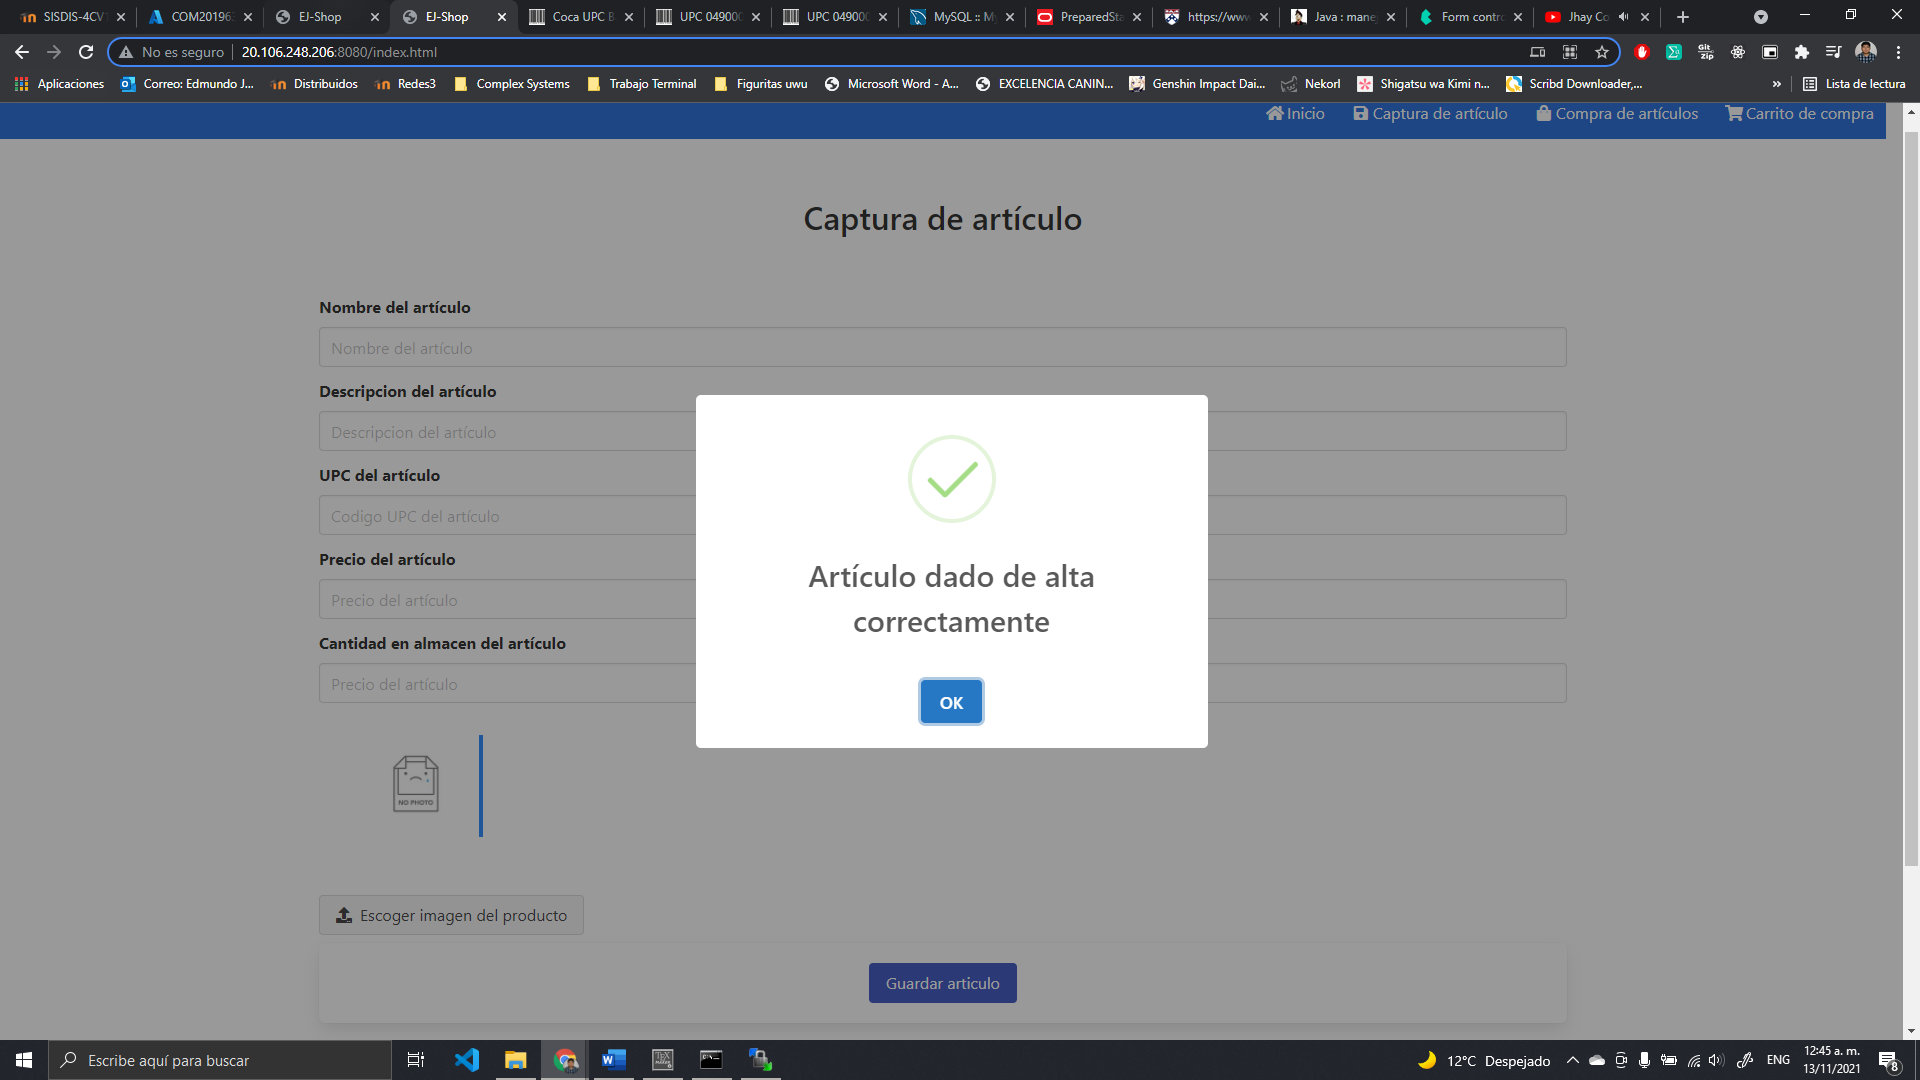
\includegraphics[scale=0.34]{resources/P1.1.png}
			\caption{Resultado 1.1. Articulo dado de alta exitosamente con foto.}\label{fig:picture}
		\end{figure}
		La siguiente prueba fue registrar un articulo sin foto como vemos en la figura 18 y en la figura 19 vemos como este fue dado de alta correctamente.
		\begin{figure}[H]
			\centering
			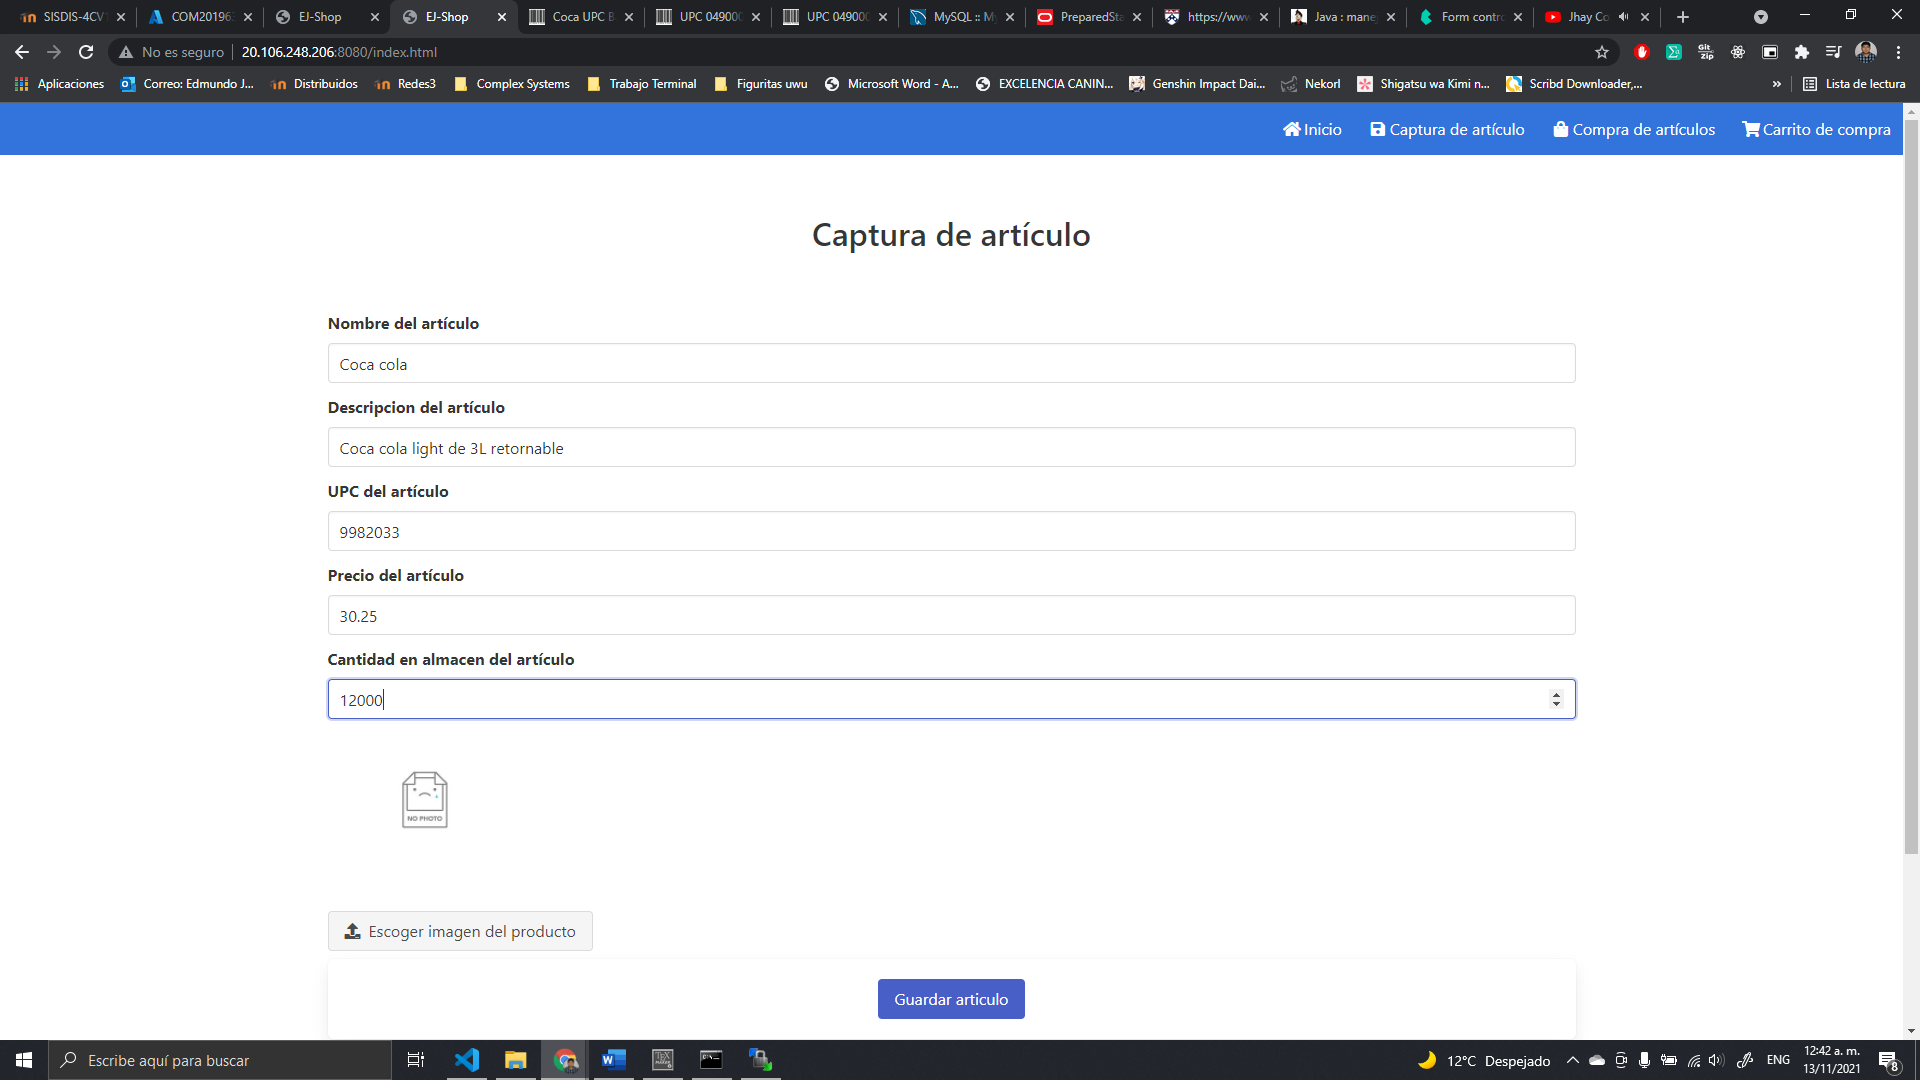
\includegraphics[scale=0.34]{resources/P1NF.png}
			\caption{Prueba 1.2. Articulo dado de alta sin foto.}\label{fig:picture}
		\end{figure}
		\begin{figure}[H]
			\centering
			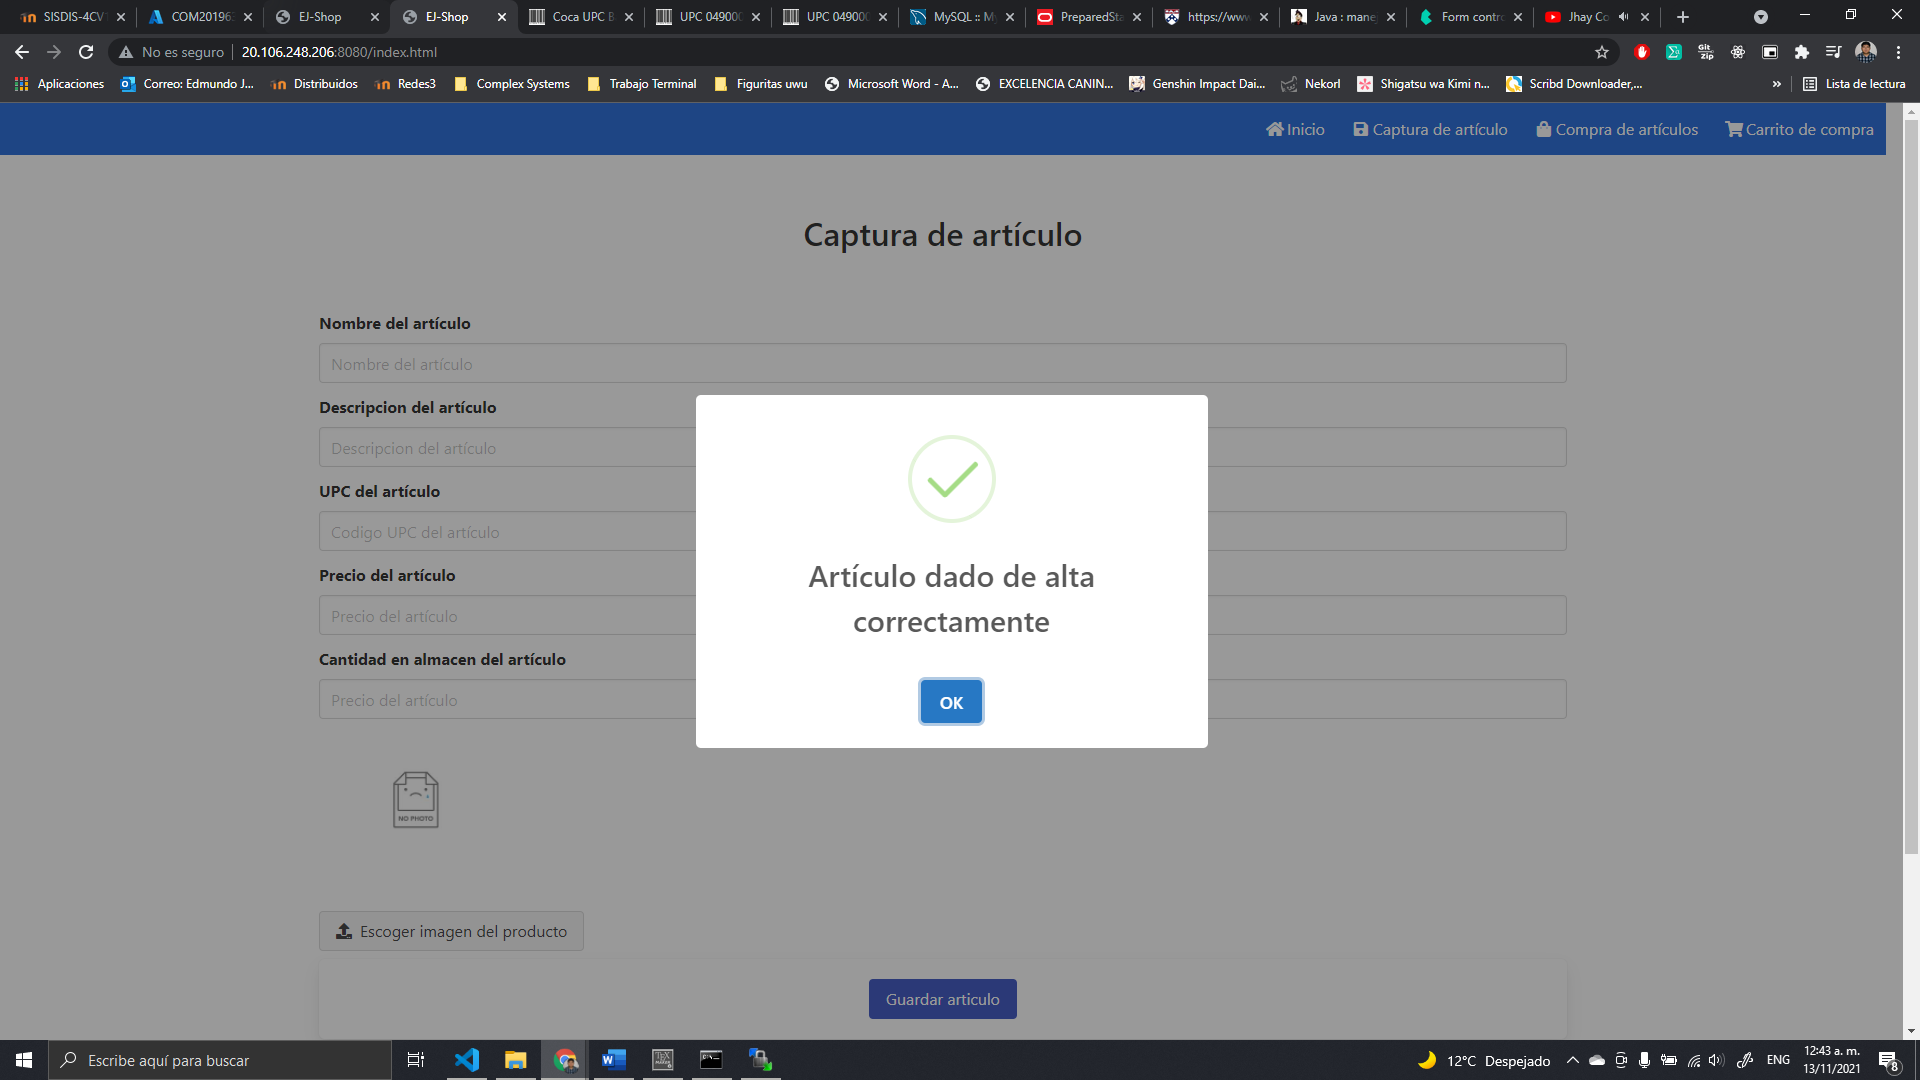
\includegraphics[scale=0.34]{resources/P1.1NF.png}
			\caption{Resultado 1.2. Articulo dado de alta exitosamente sin foto.}\label{fig:picture}
		\end{figure}
		La siguiente prueba fue ver que sucede si ponemos un UPC ya registrado con anterioridad y como vemos nos arroja un error de que el UPC ya existe, esto lo podemos ver en la figura 20, mencionar que este producto fue guardado en la base de datos pero evidentemente usando un UPC inexistente.
		\begin{figure}[H]
			\centering
			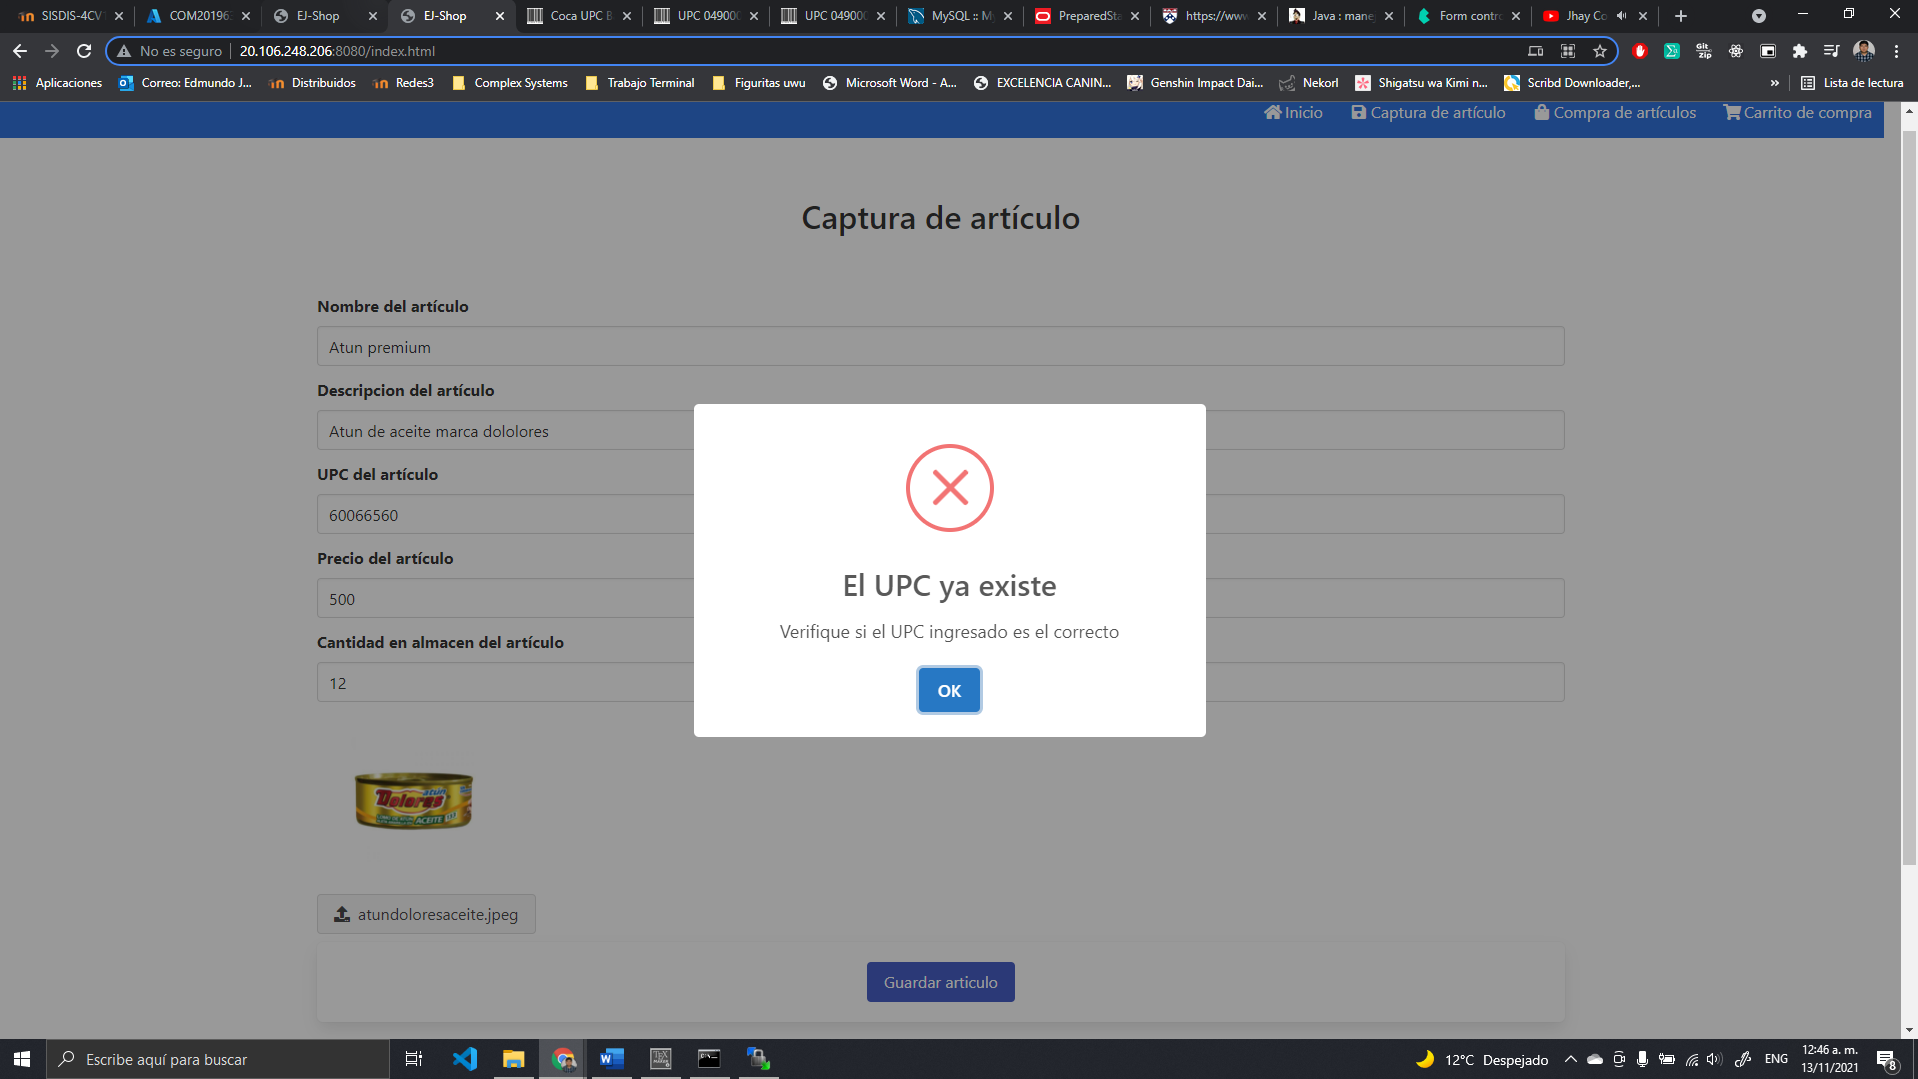
\includegraphics[scale=0.34]{resources/P1.ERROR.png}
			\caption{Resultado 1.3. Articulo con UPC ya guardo anteriormente.}\label{fig:picture}
		\end{figure}
		Como ultima prueba se realizo un registro desde el celular, esto lo podemos ver en las figuras 21 y 22, añadir que en la figura 21 podemos ver en la parte superior una famosa burger navbaren la que si damos click se nos despliega las opciones que mencionamos al inicio. Finalmente en la figura 23 podemos ver como el articulo fue dado de alta de forma correcta
		\begin{figure}[H]
			\centering
			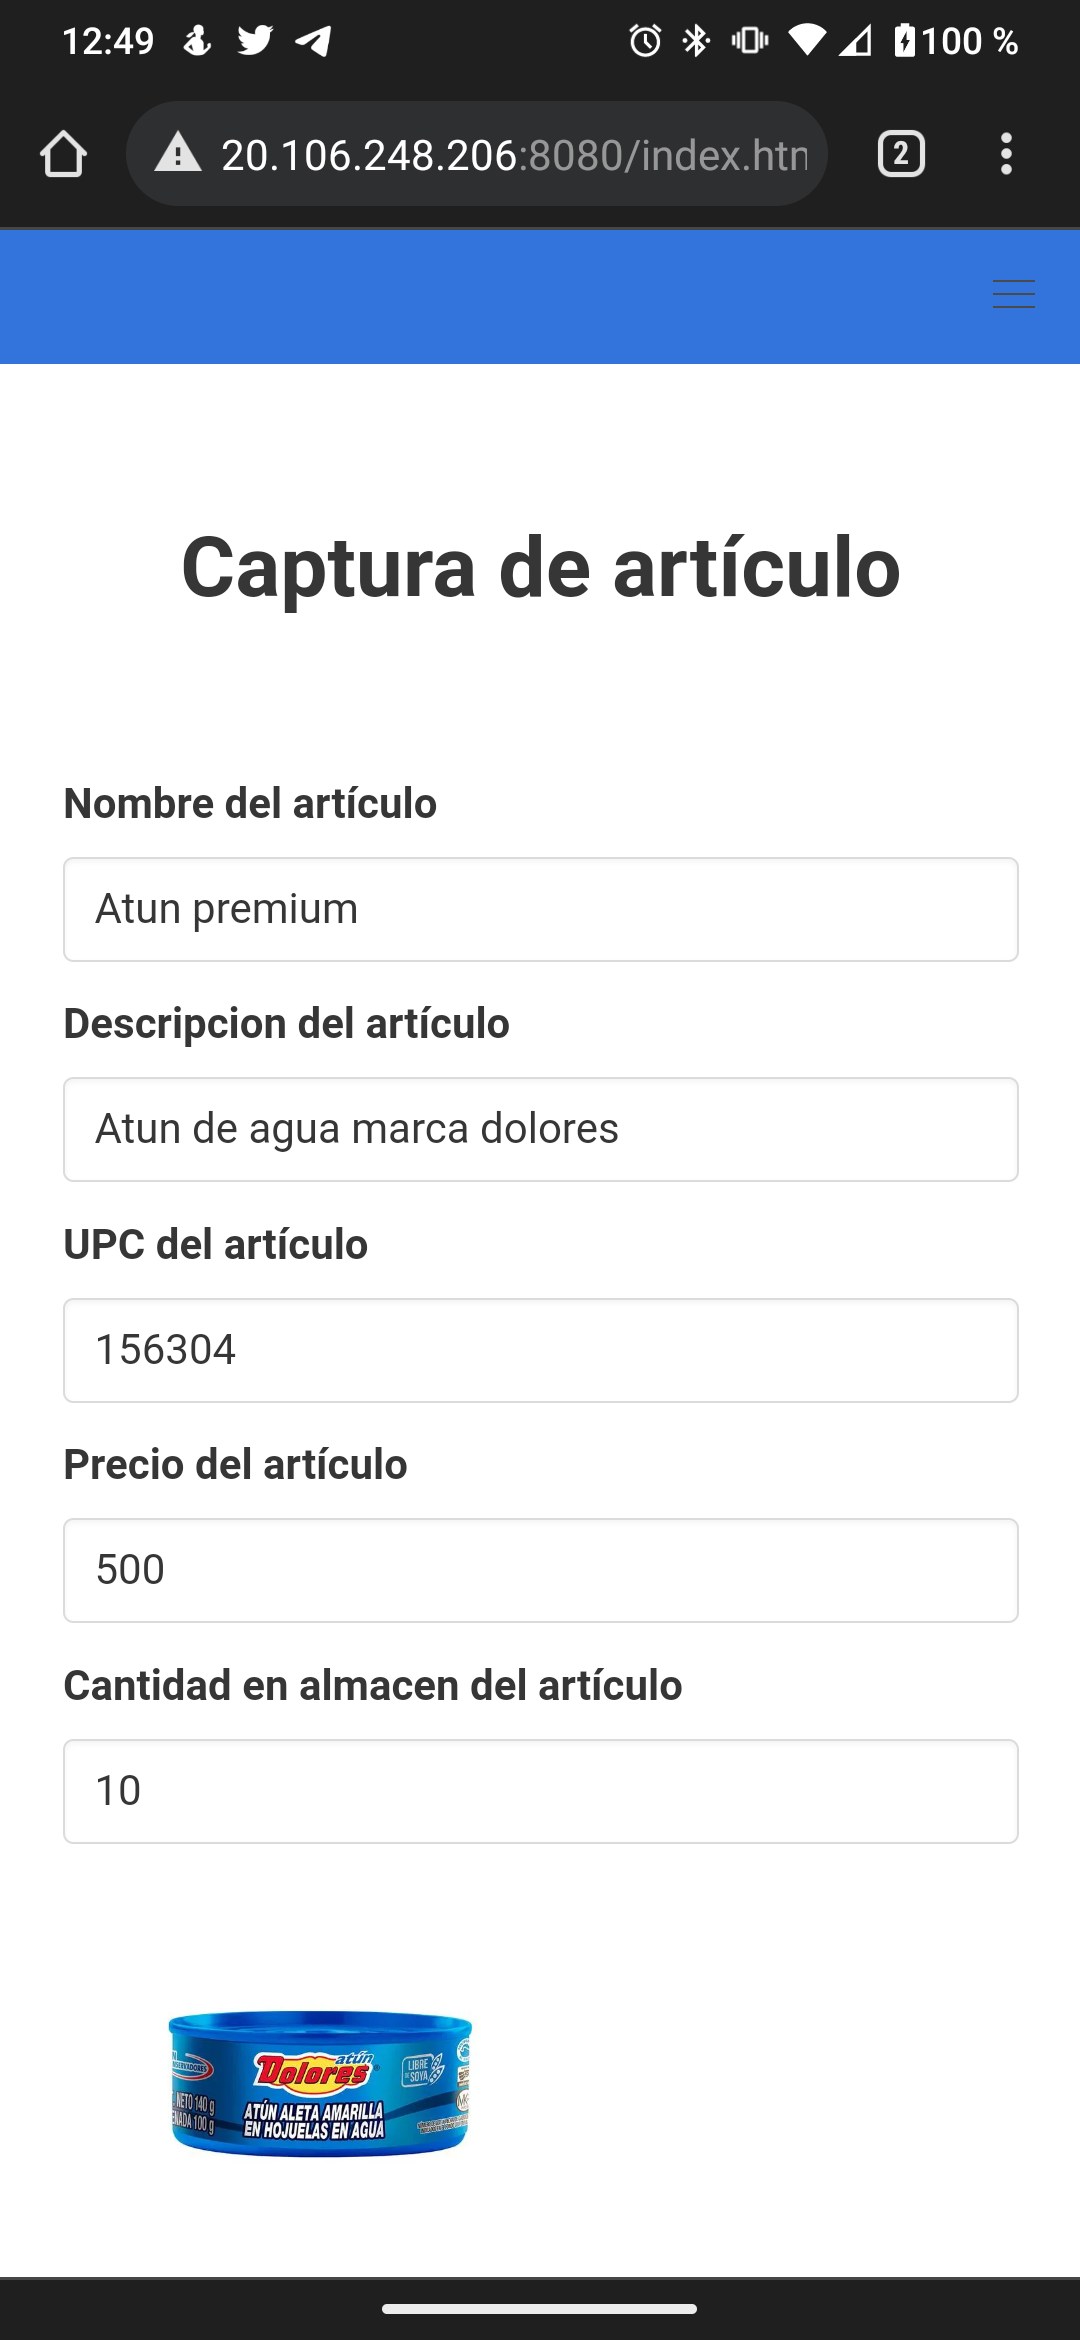
\includegraphics[scale=0.27]{resources/Screenshot_20211113-004906.png}
			\caption{Prueba 1.4. Articulo dado de alta con foto en celular.}\label{fig:picture}
		\end{figure}
		\begin{figure}[H]
			\centering
			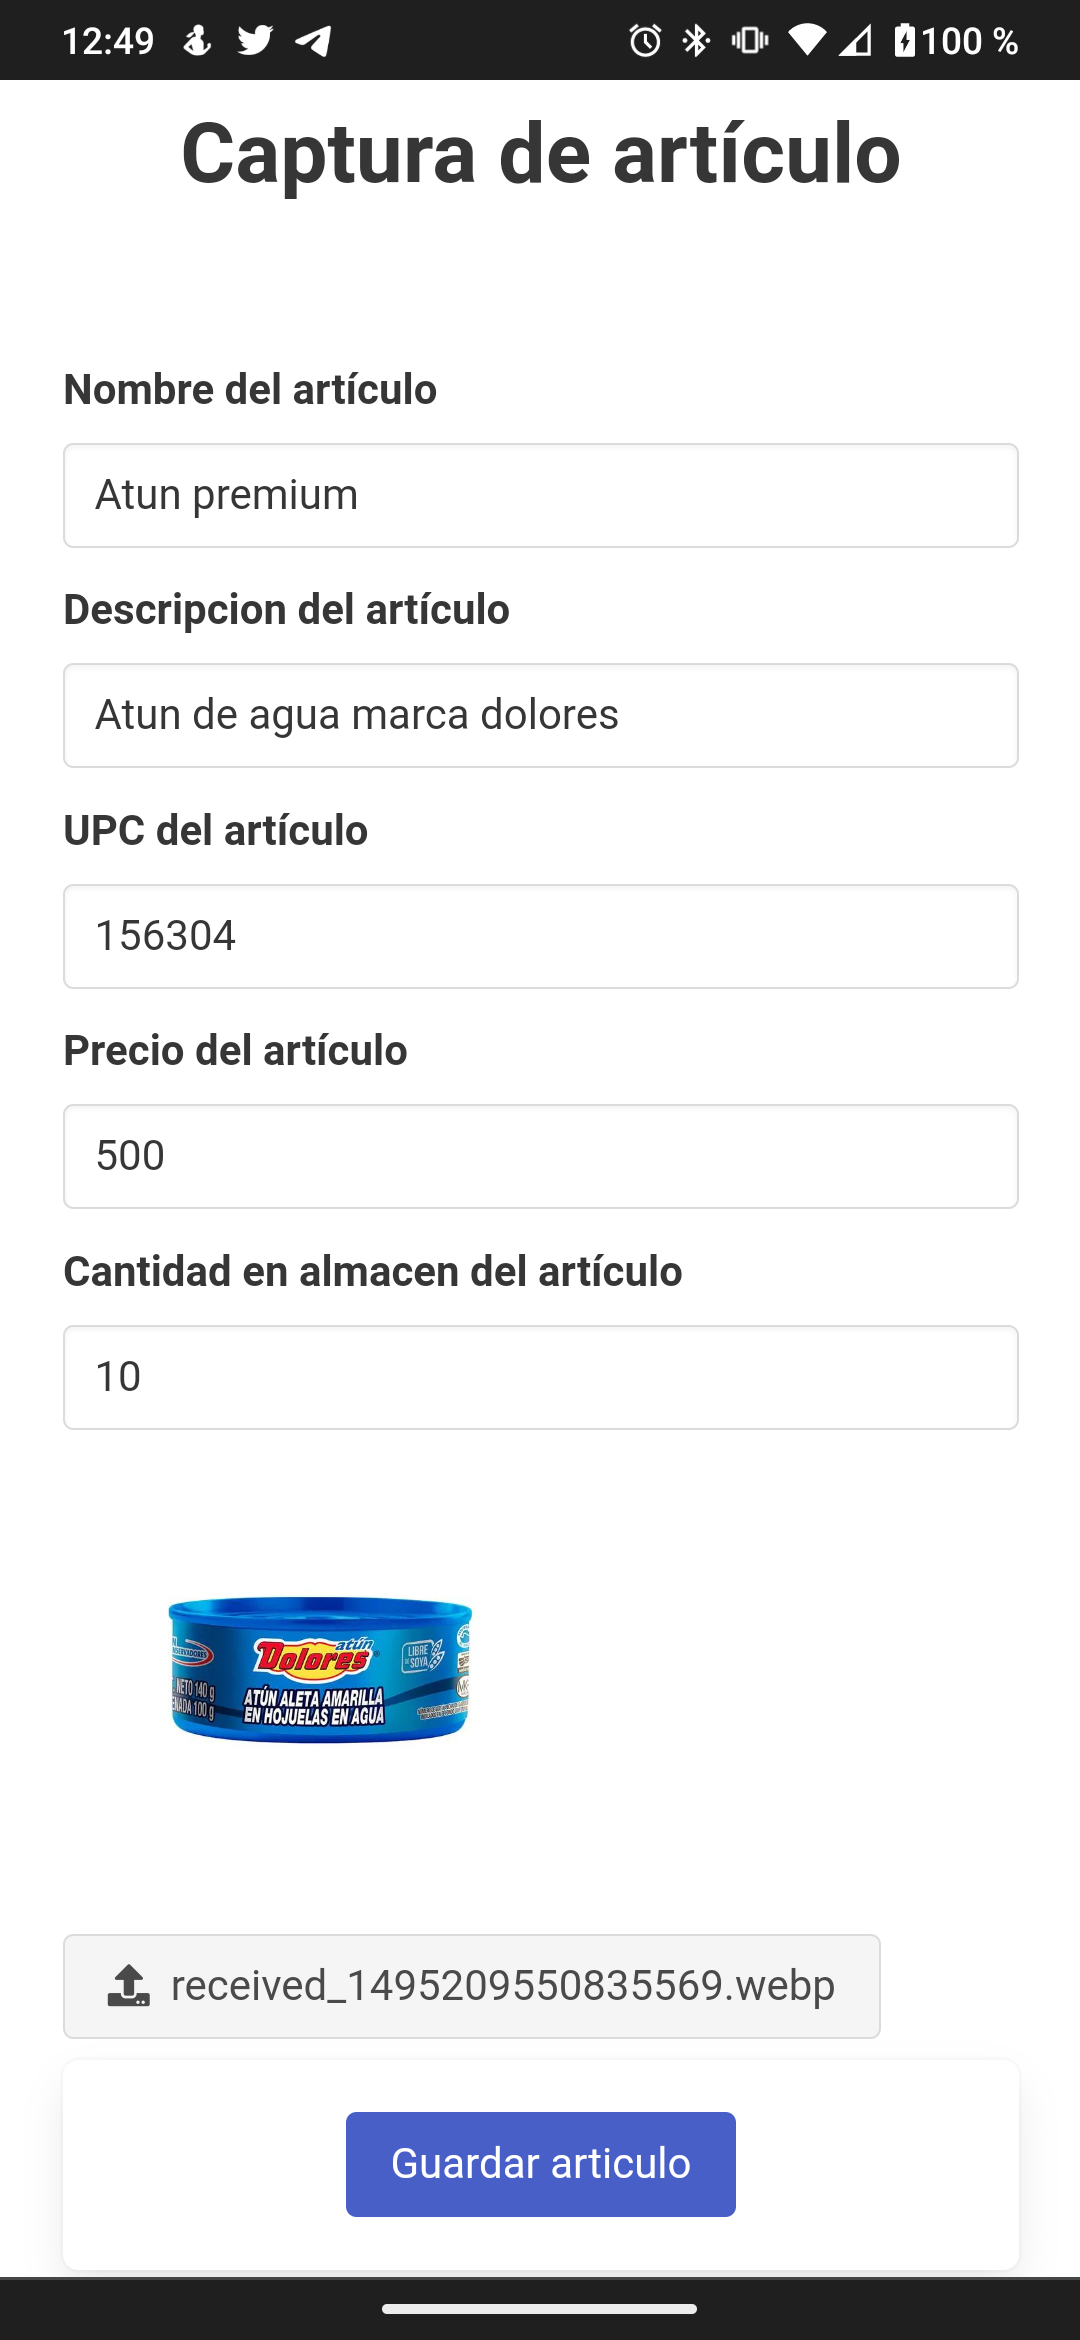
\includegraphics[scale=0.27]{resources/Screenshot_20211113-004912.png}
			\caption{Prueba 1.4. Articulo dado de alta con foto en celular.}\label{fig:picture}
		\end{figure}
		\begin{figure}[H]
			\centering
			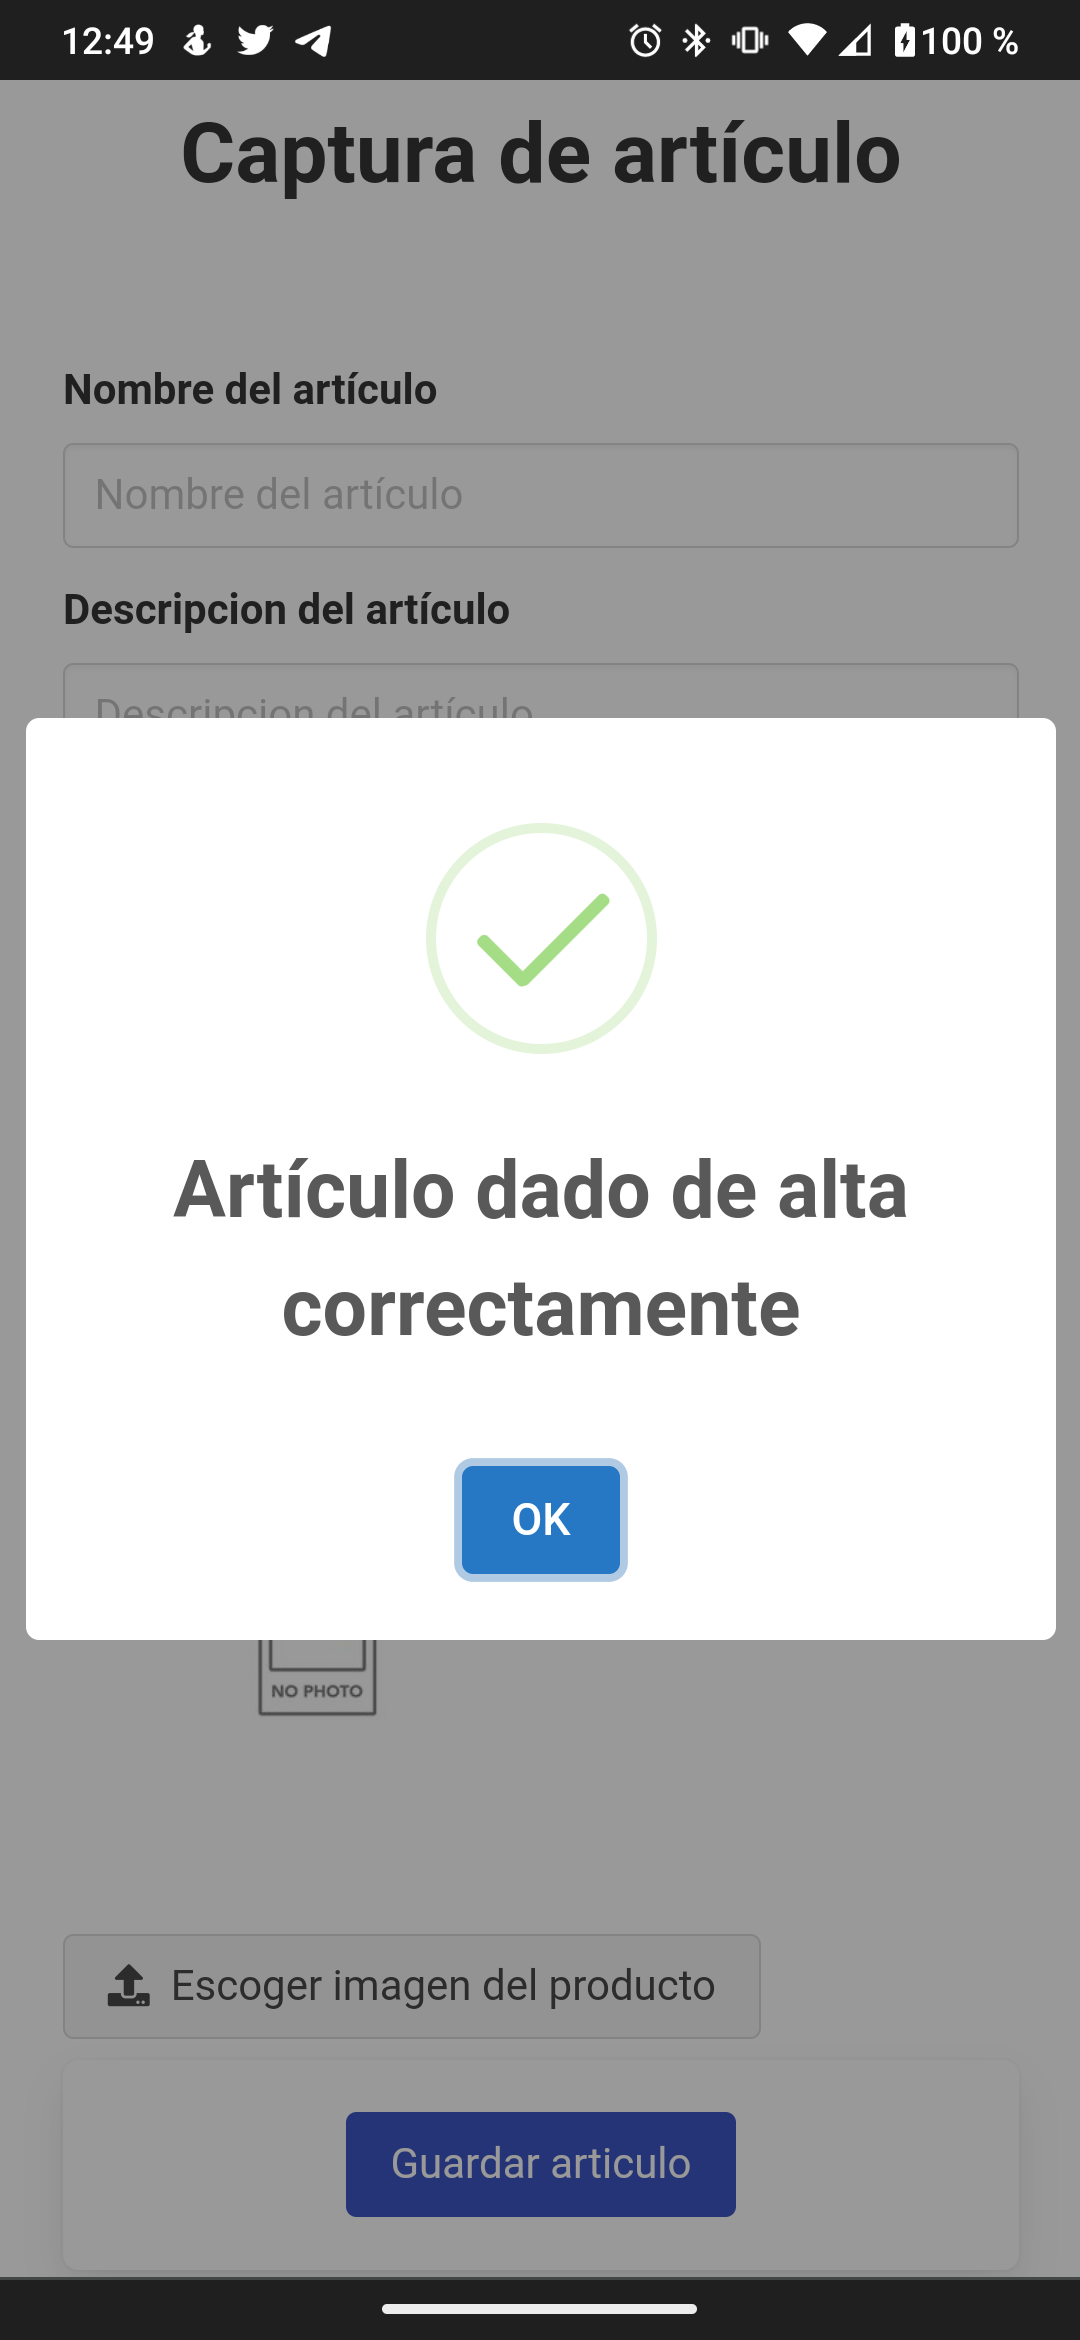
\includegraphics[scale=0.27]{resources/Screenshot_20211113-004916.png}
			\caption{Resultado 1.4. Articulo dado de alta exitosamente con foto en celular.}\label{fig:picture}
		\end{figure}
		Finalmente veamos la base de datos resultante de estas pruebas junto con otros artículos anteriormente creados, esto lo podemos ver en la figura 24 y en las figuras 25 a la 28 podemos ver la pagina de inicio y como podemos ver todos los artículos dados de alta, esto tanto en computadora como en celular.
		\begin{figure}[H]
			\centering
			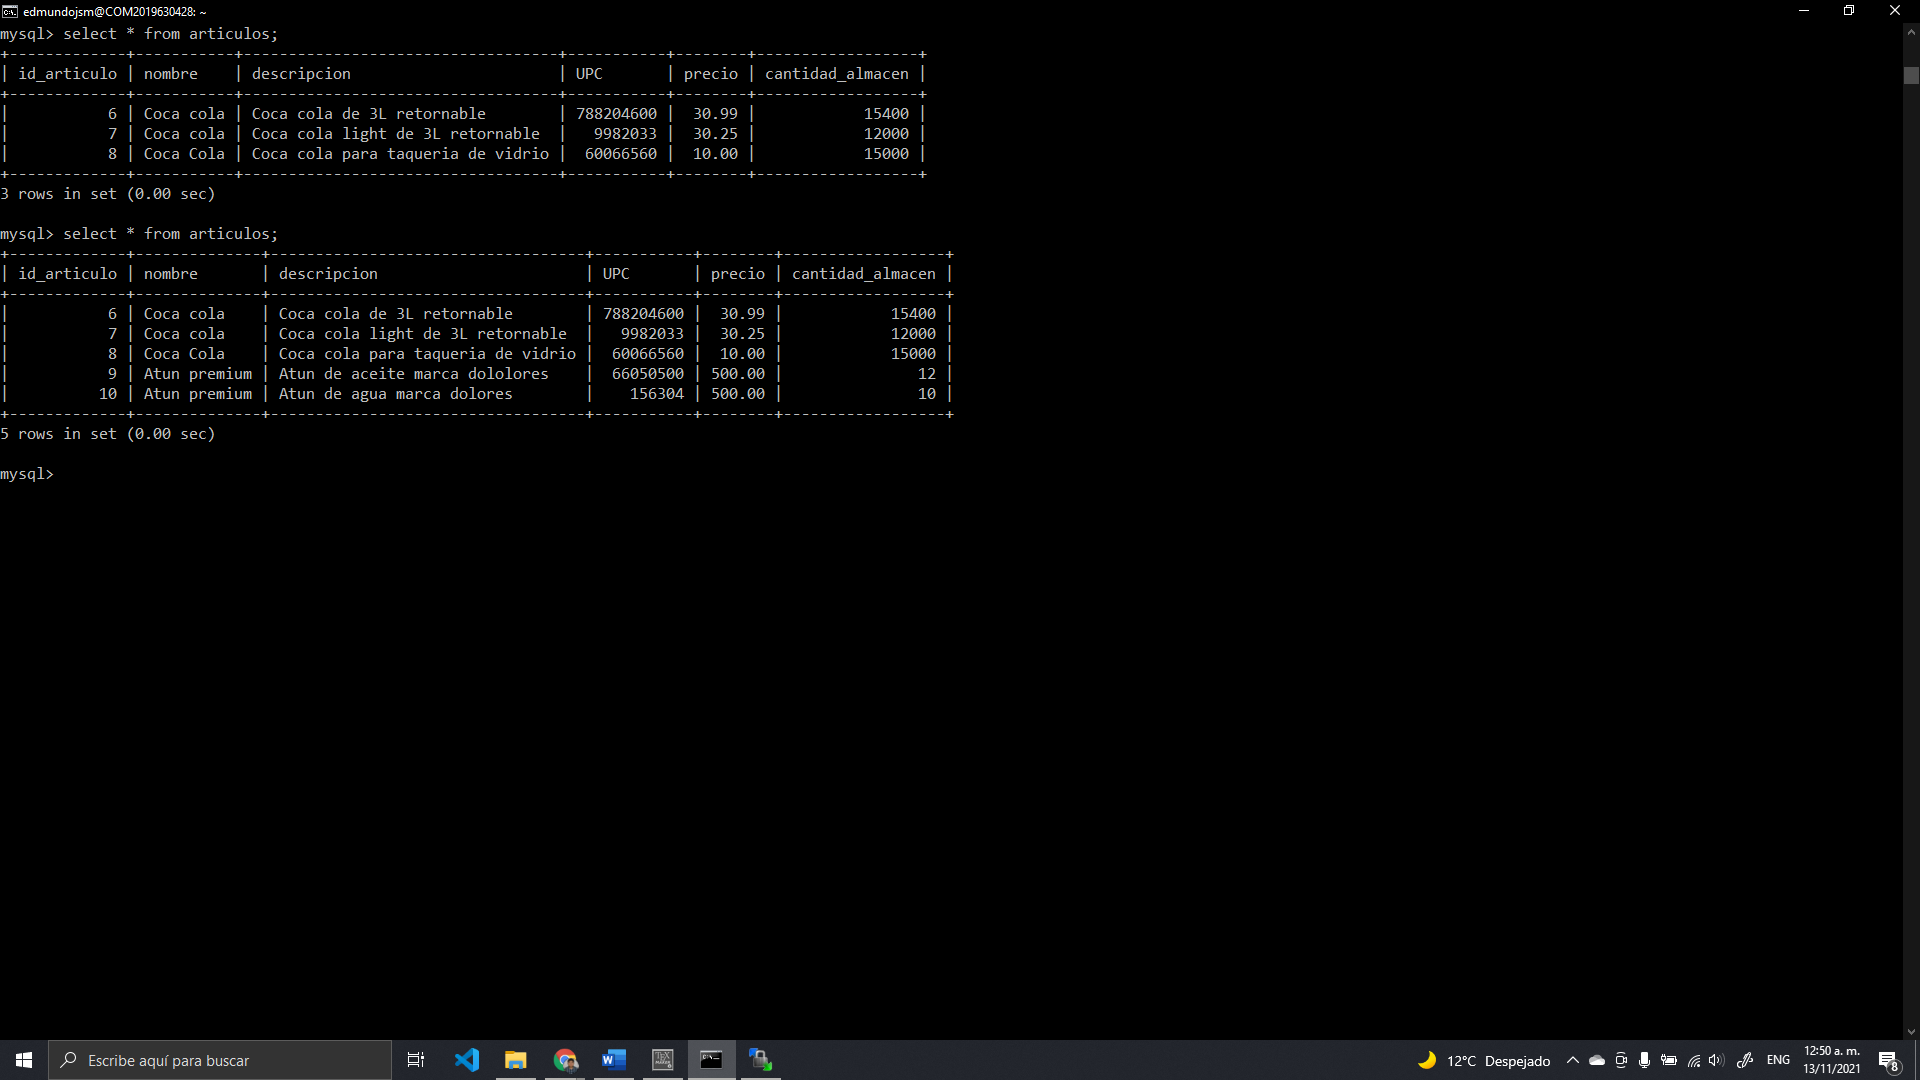
\includegraphics[scale=0.34]{resources/bdp1.png}
			\caption{Base de datos con los artículos dados de alta.}\label{fig:picture}
		\end{figure}
		\begin{figure}[H]
			\centering
			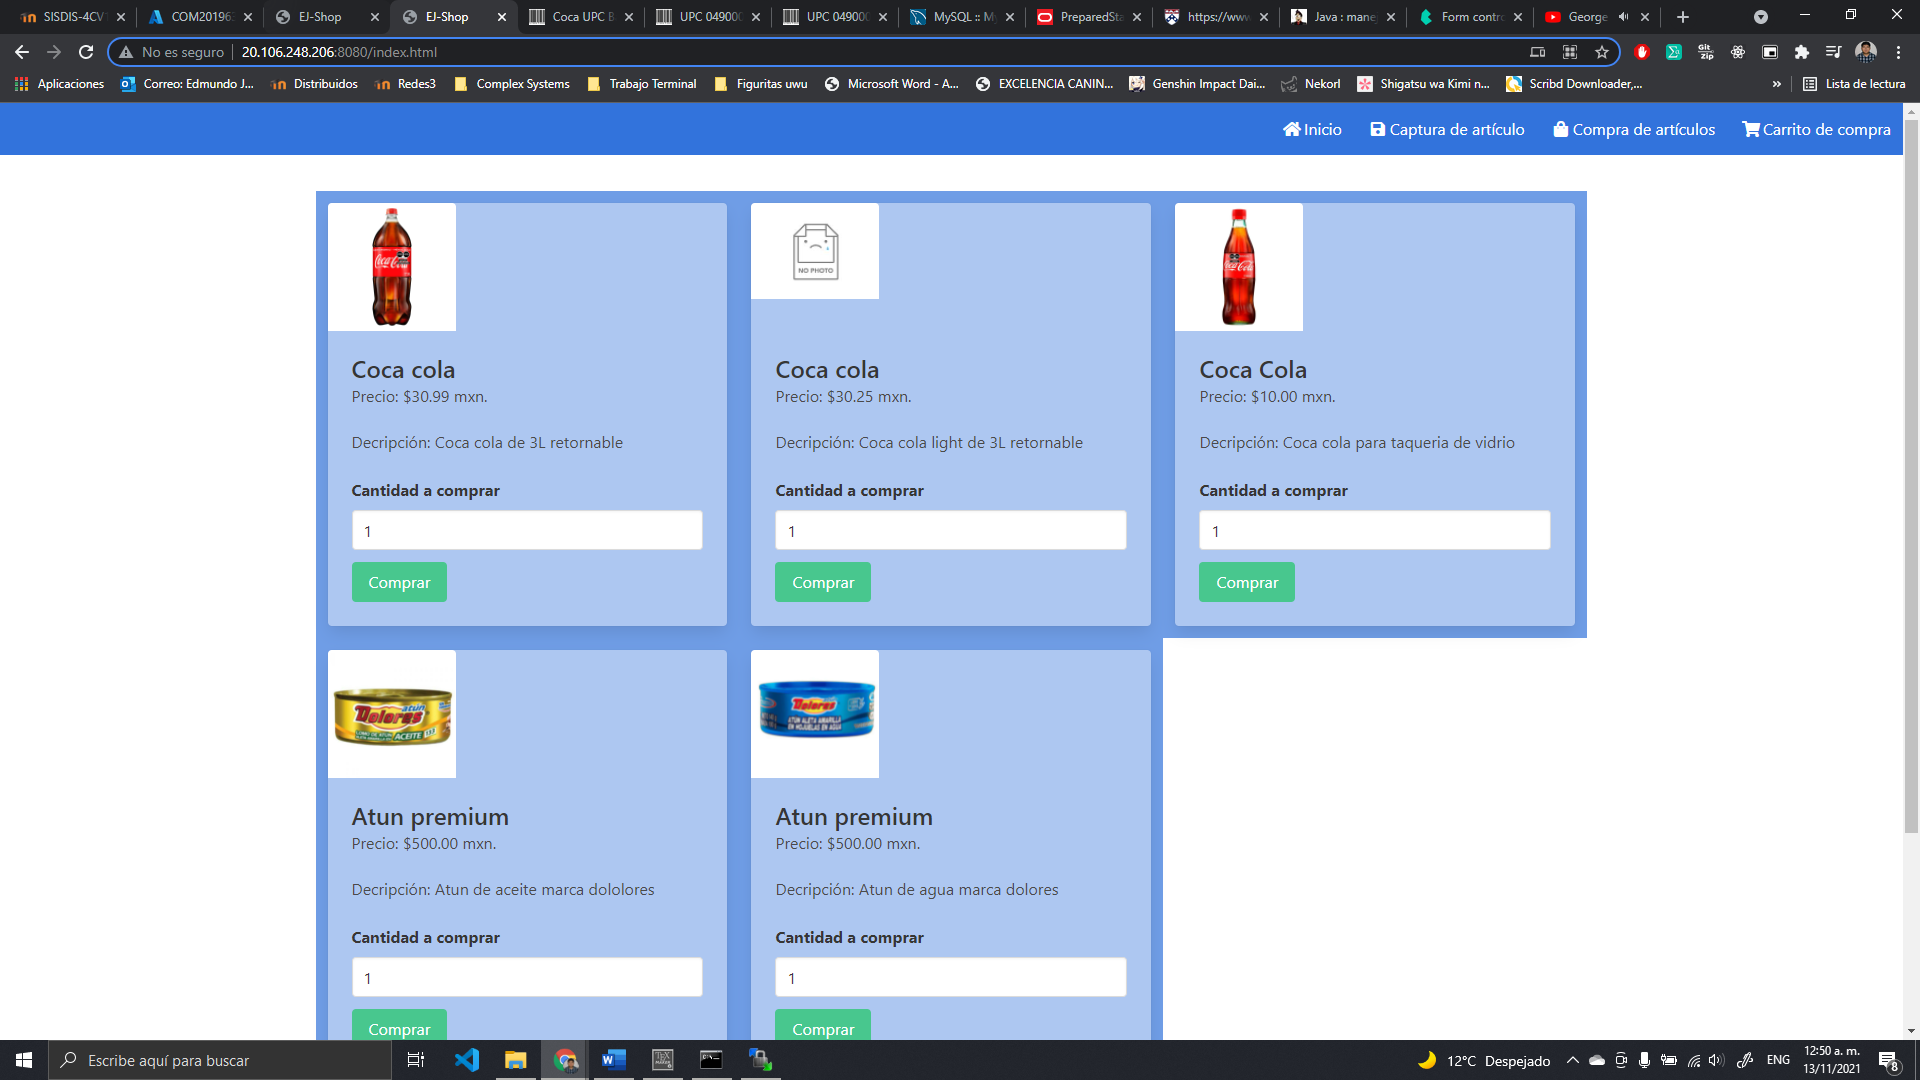
\includegraphics[scale=0.34]{resources/inicio_productos.png}
			\caption{Pagina de inicio del sistema.}\label{fig:picture}
		\end{figure}
		\begin{figure}[H]
			\centering
			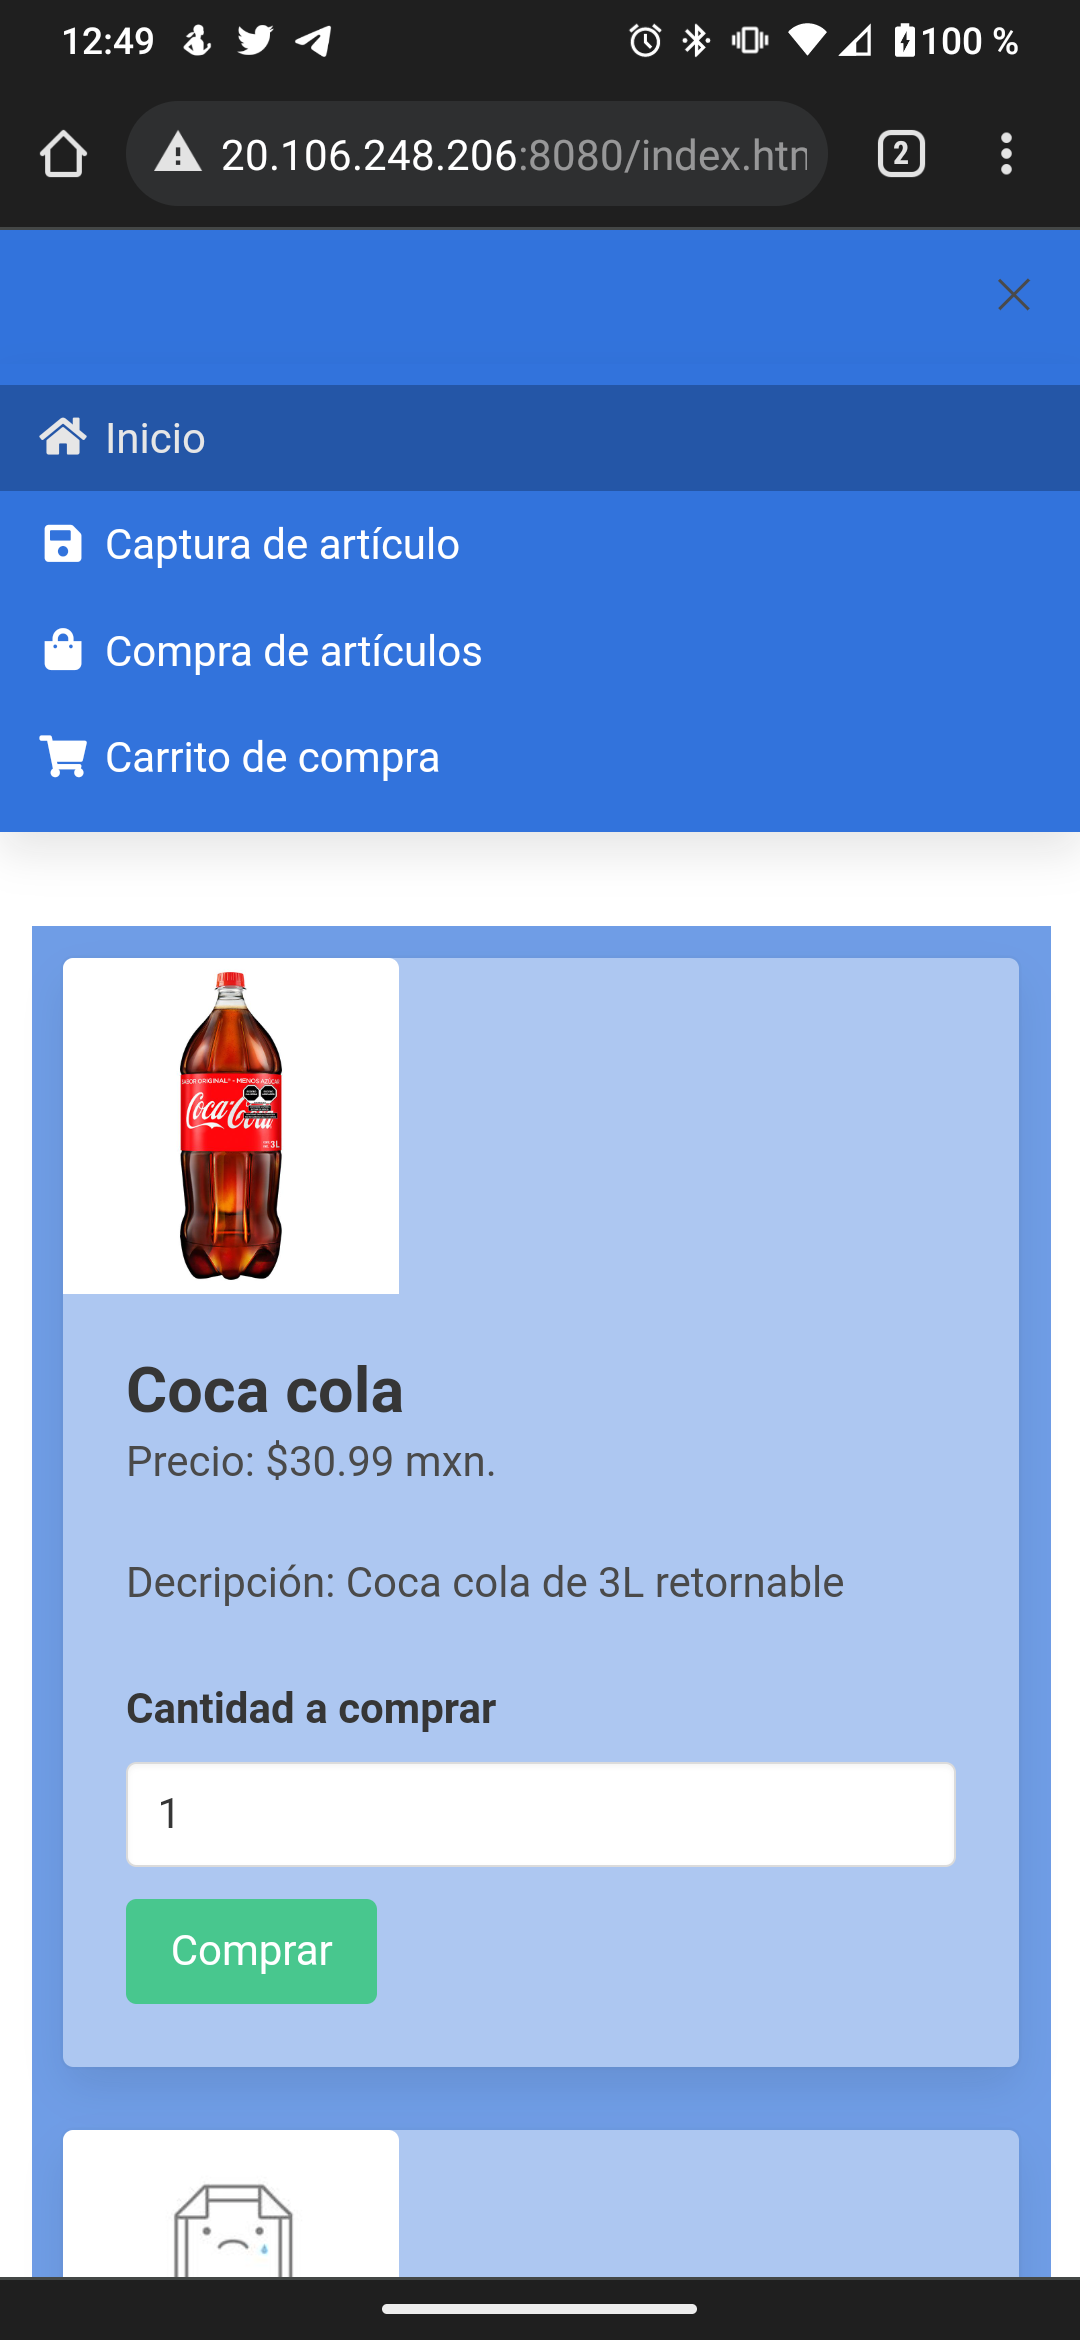
\includegraphics[scale=0.27]{resources/Screenshot_20211113-004941.png}
			\caption{Pagina de inicio del sistema en celular. Parte 1.}\label{fig:picture}
		\end{figure}
		\begin{figure}[H]
			\centering
			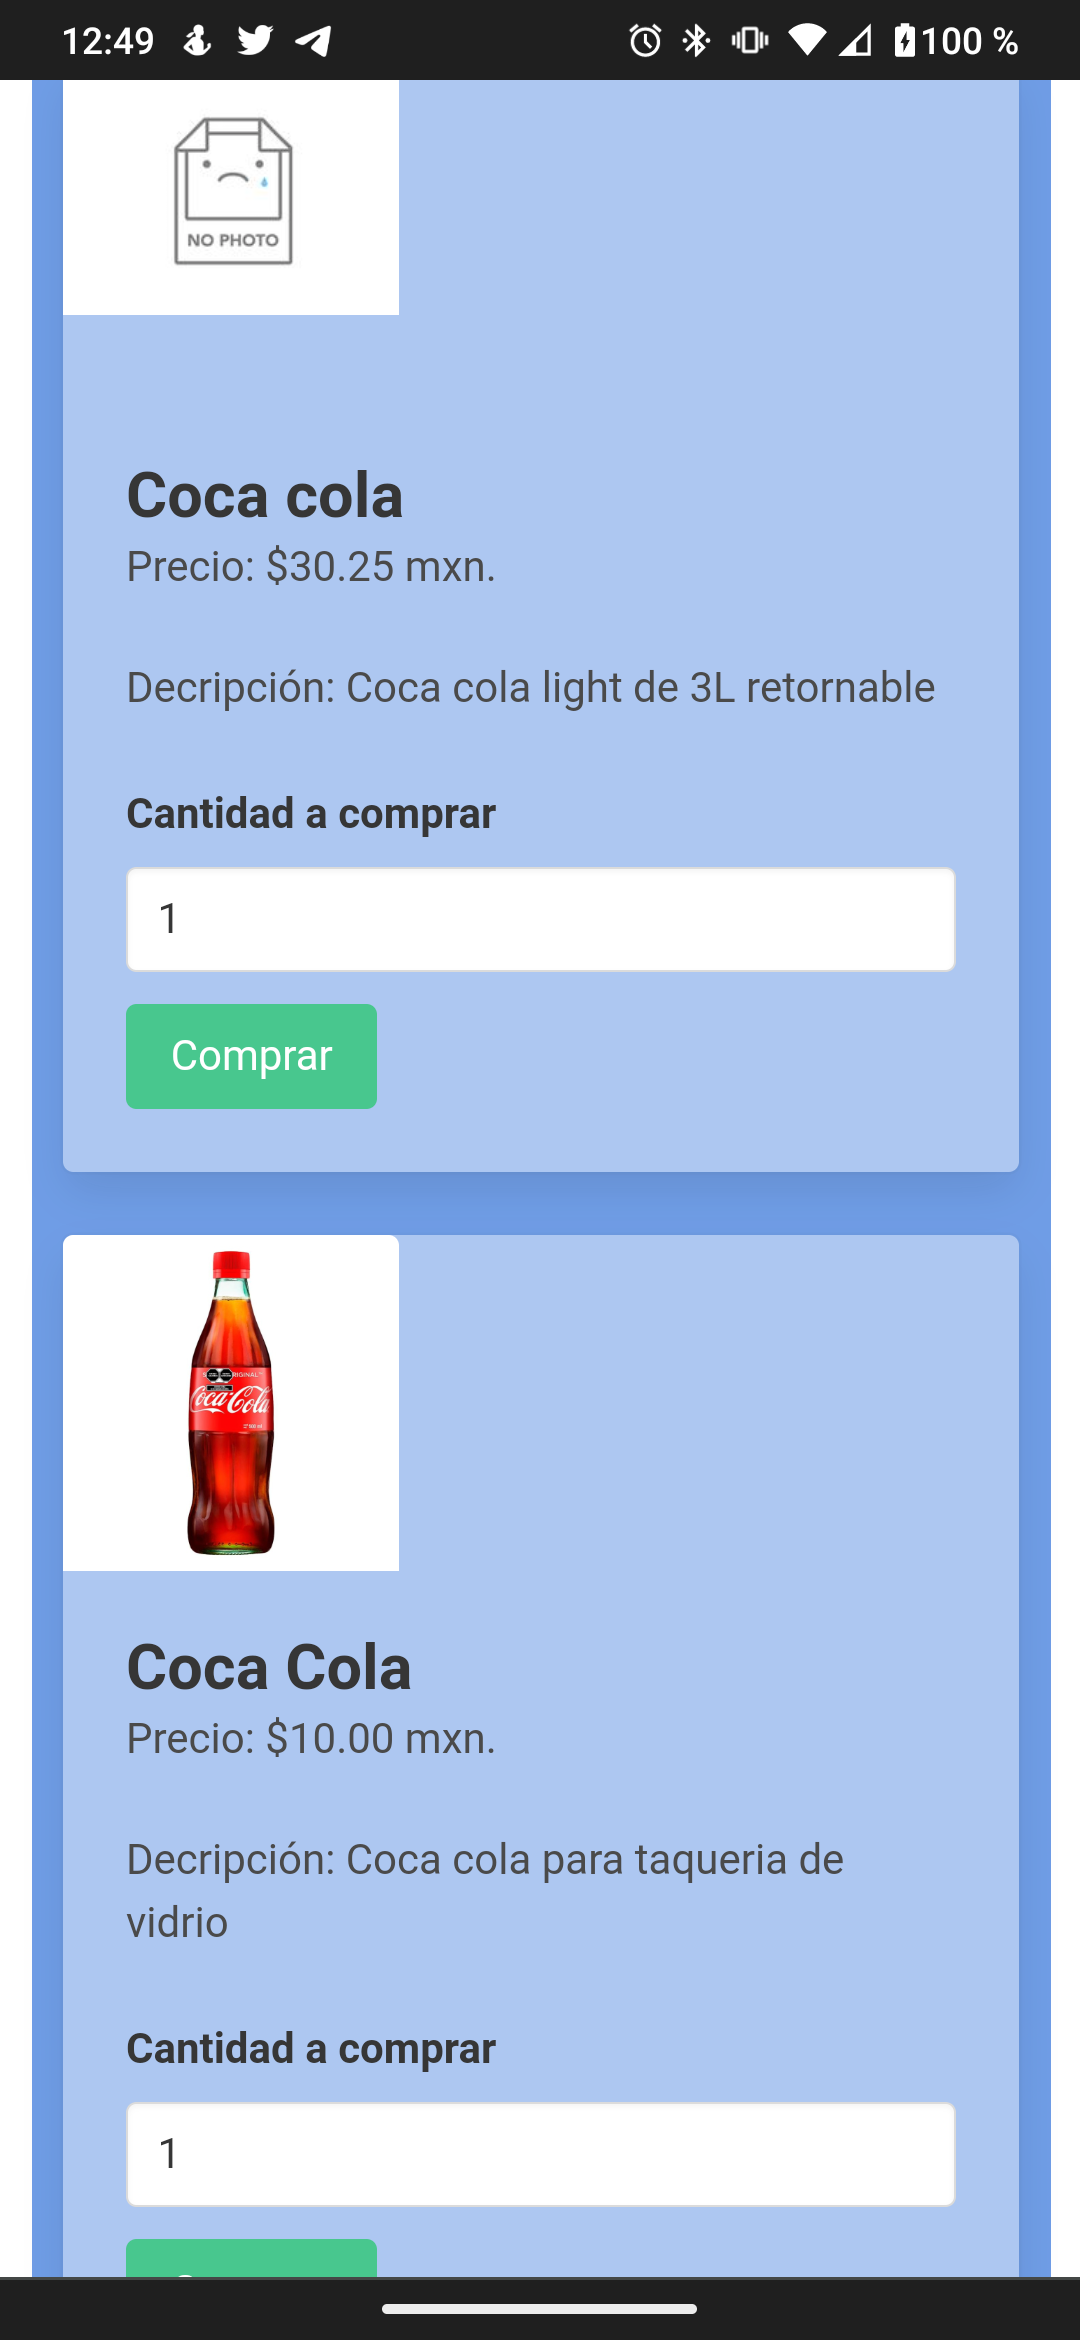
\includegraphics[scale=0.27]{resources/Screenshot_20211113-004950.png}
			\caption{Pagina de inicio del sistema en celular. Parte 2.}\label{fig:picture}
		\end{figure}
		\begin{figure}[H]
			\centering
			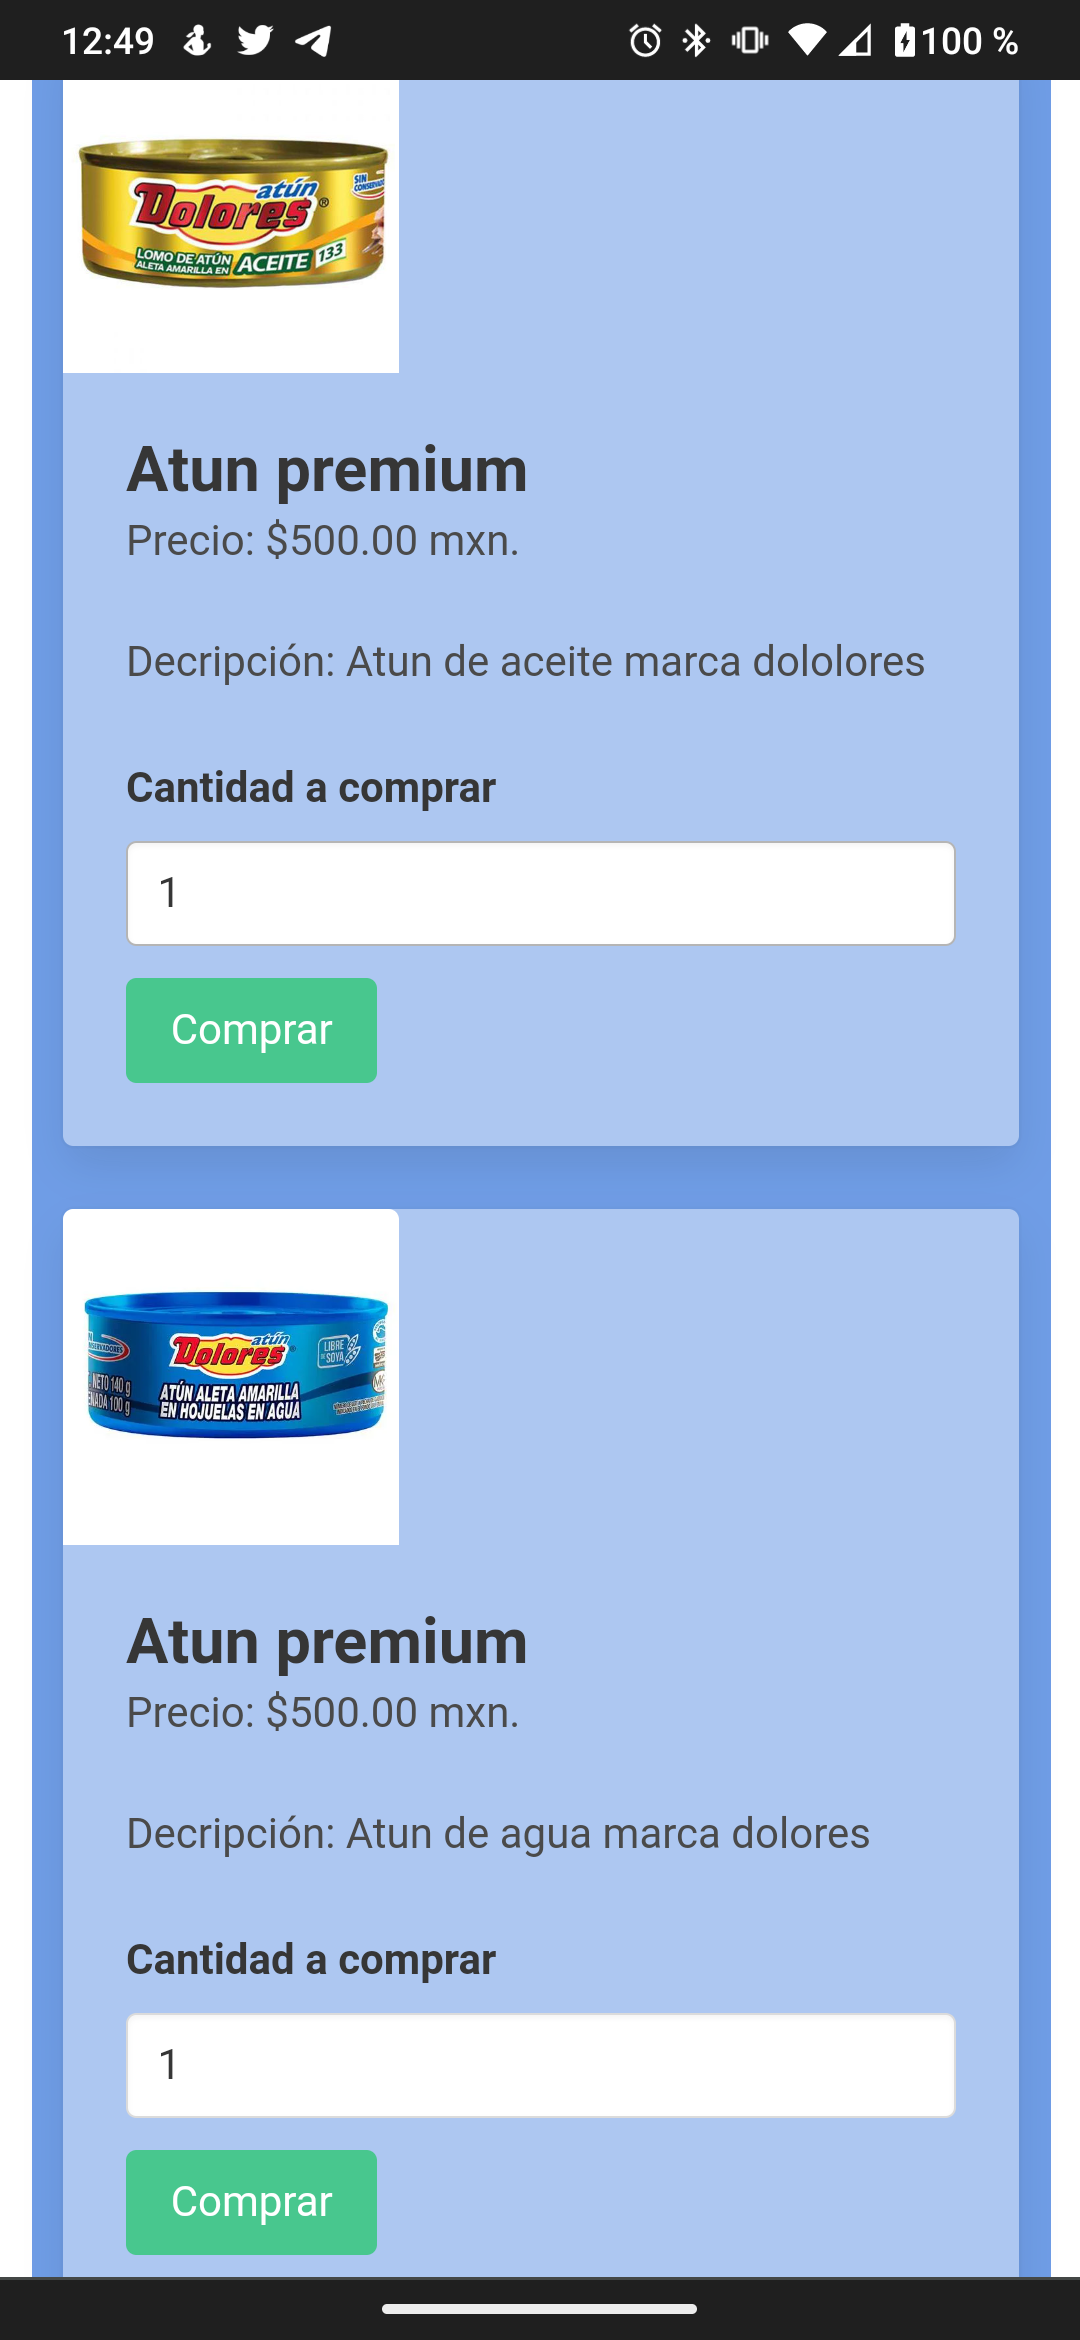
\includegraphics[scale=0.27]{resources/Screenshot_20211113-004956.png}
			\caption{Pagina de inicio del sistema en celular. Parte 3.}\label{fig:picture}
		\end{figure}
		\subsection{Prueba 2. Búsqueda de artículos}
		Ahora vemos como se realizan la búsqueda de articulos, al dar click en la opción de Compra de artículos nos sale la opción de buscar artículos con base a una palabra ingresada, las pruebas que se hicieron fueron solo en la computadora, sin embargo, en la siguiente prueba que sera la compra de artículos se hacen también en el celular por lo cual cubrimos este punto. Ahora si veamos las pruebas, estas serán de la figura 29 a la 33.
		\begin{figure}[H]
			\centering
			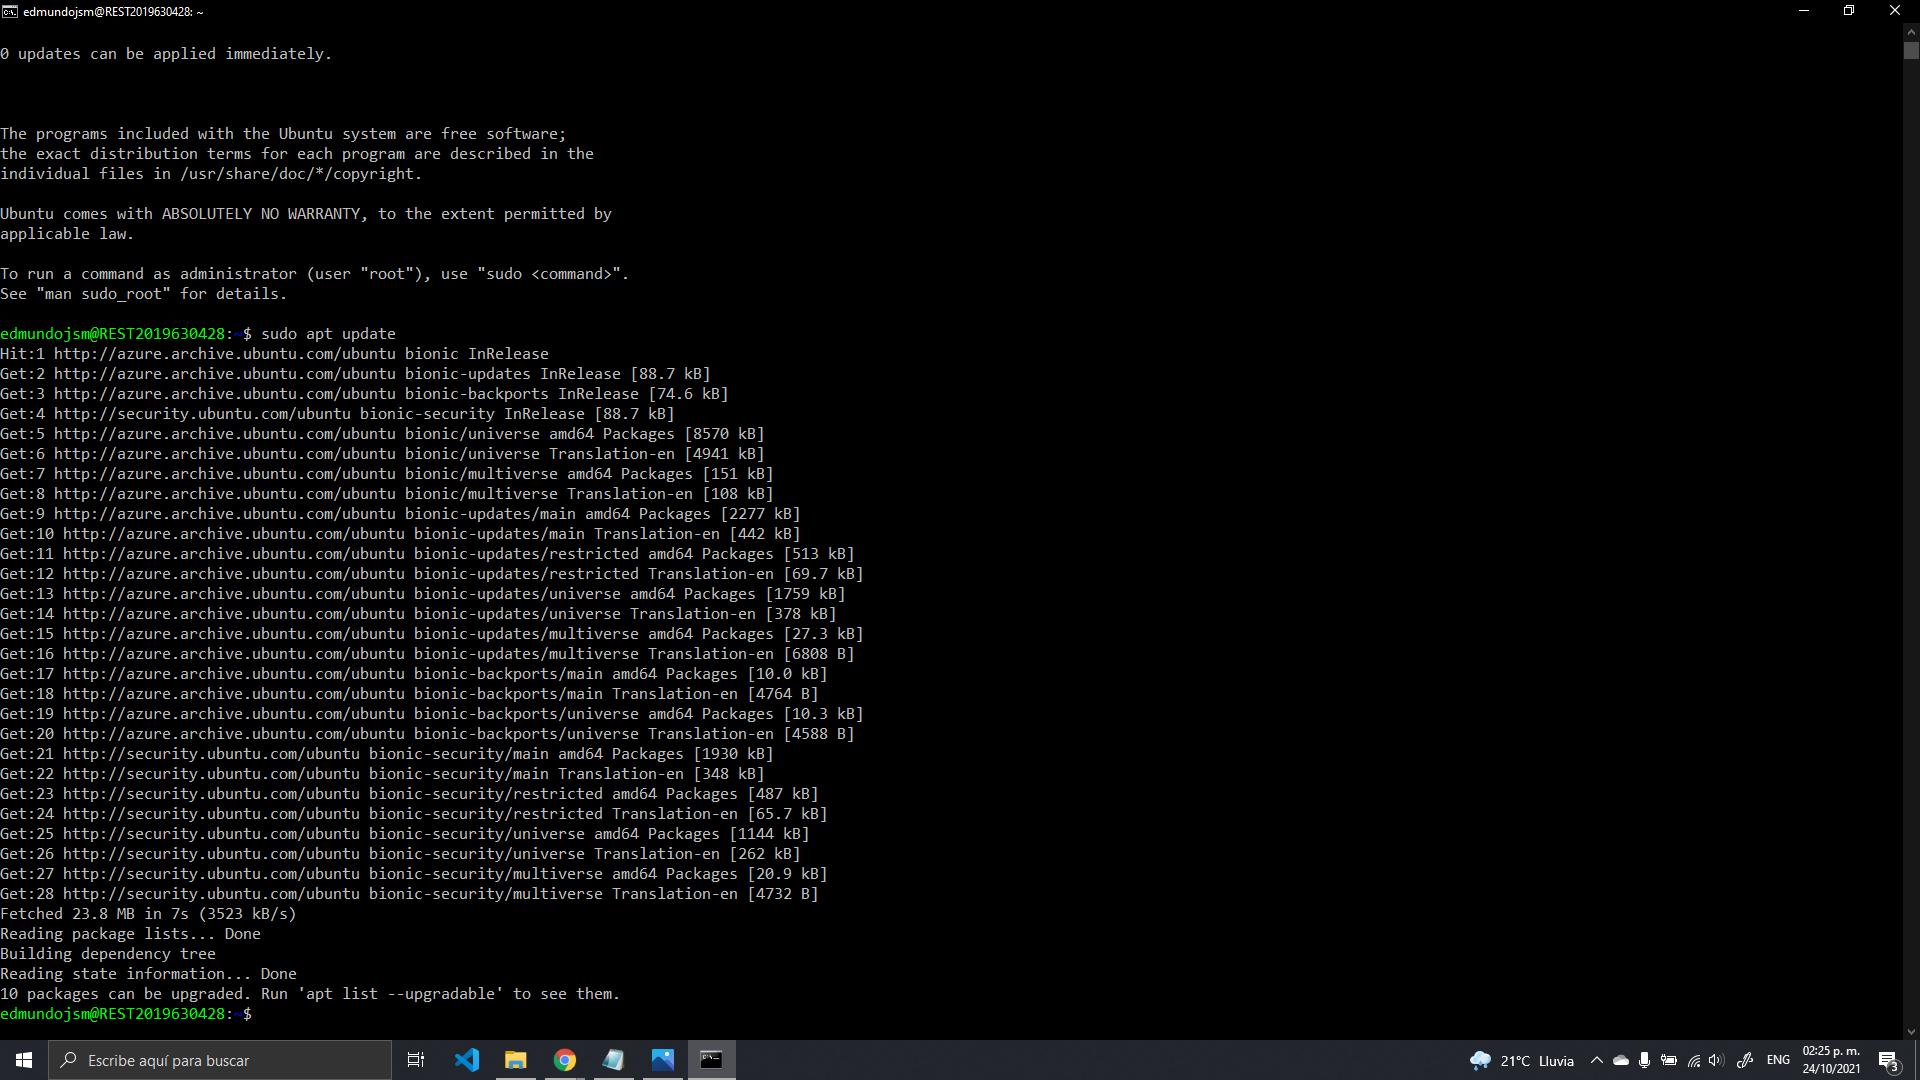
\includegraphics[scale=0.34]{resources/p2.1.png}
			\caption{Ingresar palabra a buscar los artículos.}\label{fig:picture}
		\end{figure}
		\begin{figure}[H]
			\centering
			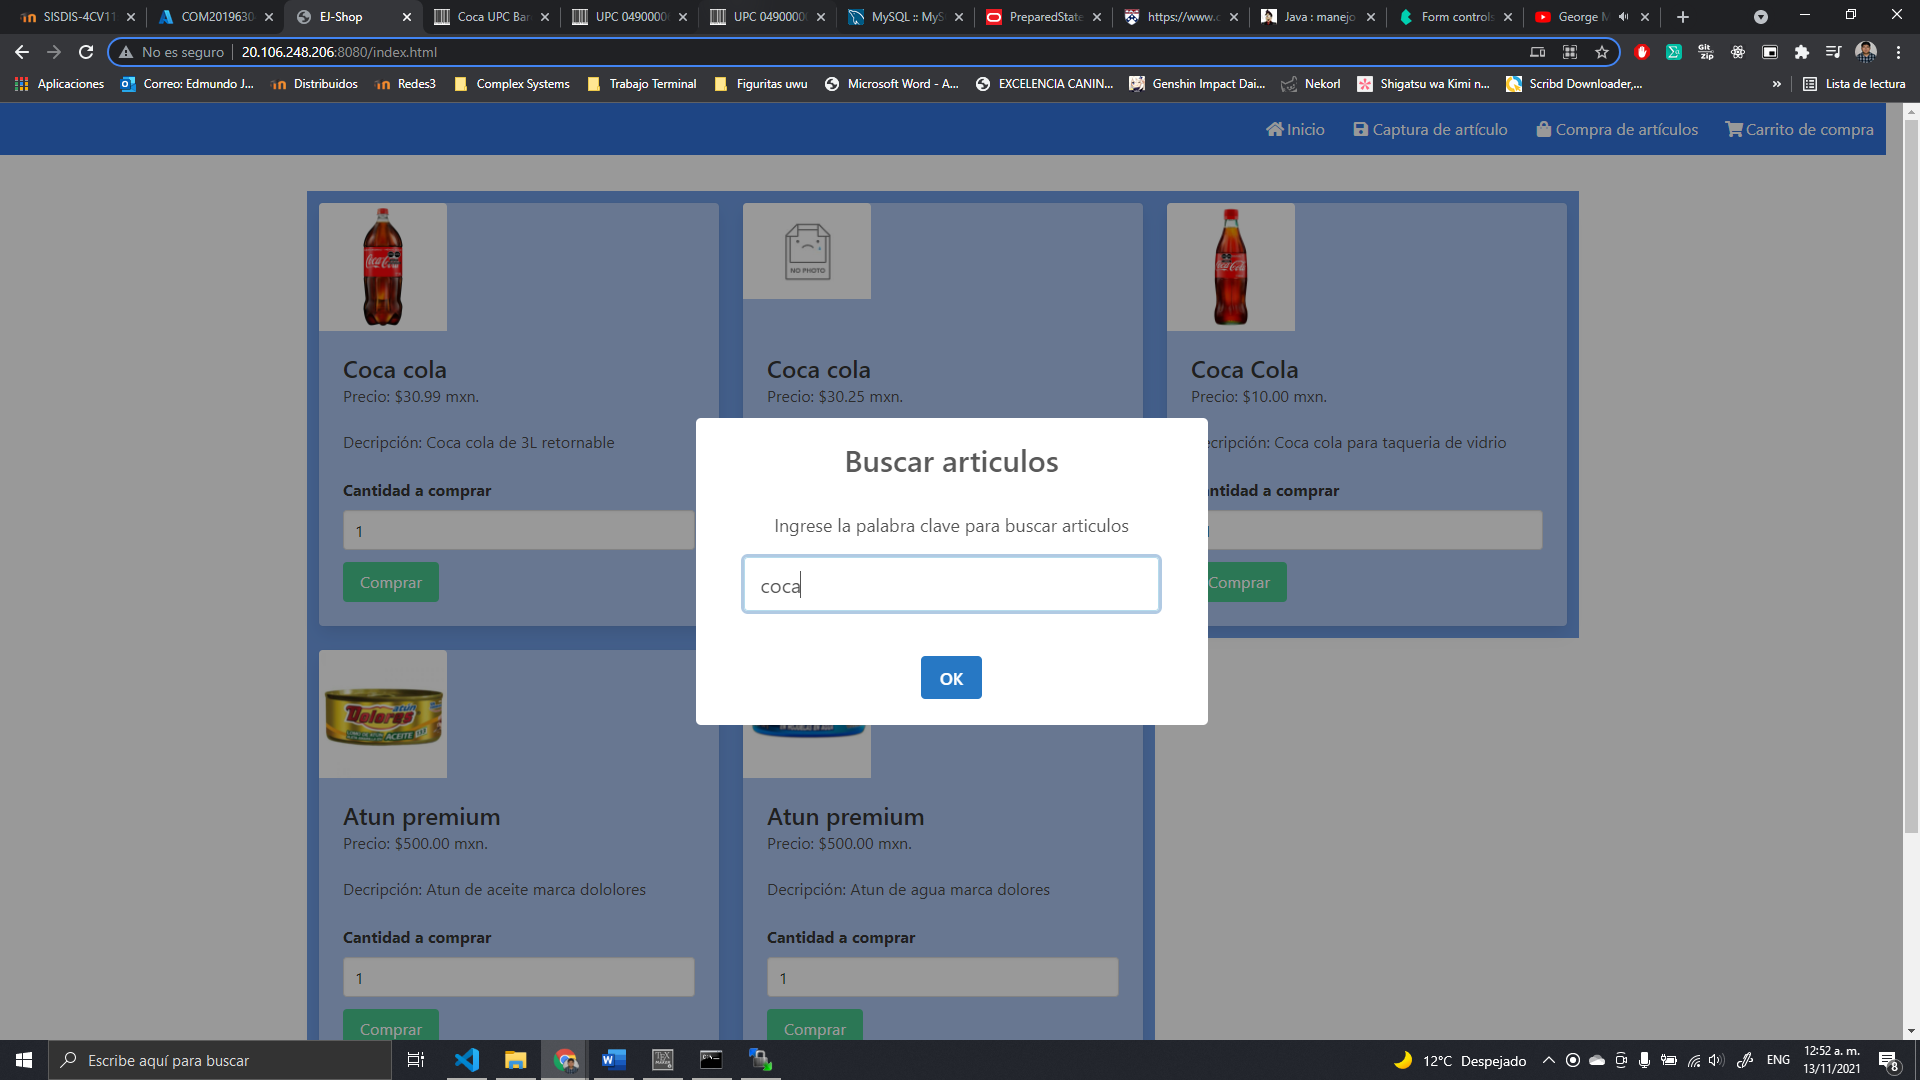
\includegraphics[scale=0.34]{resources/p2.1.1.png}
			\caption{Buscando palabra ``coca''.}\label{fig:picture}
		\end{figure}
		\begin{figure}[H]
			\centering
			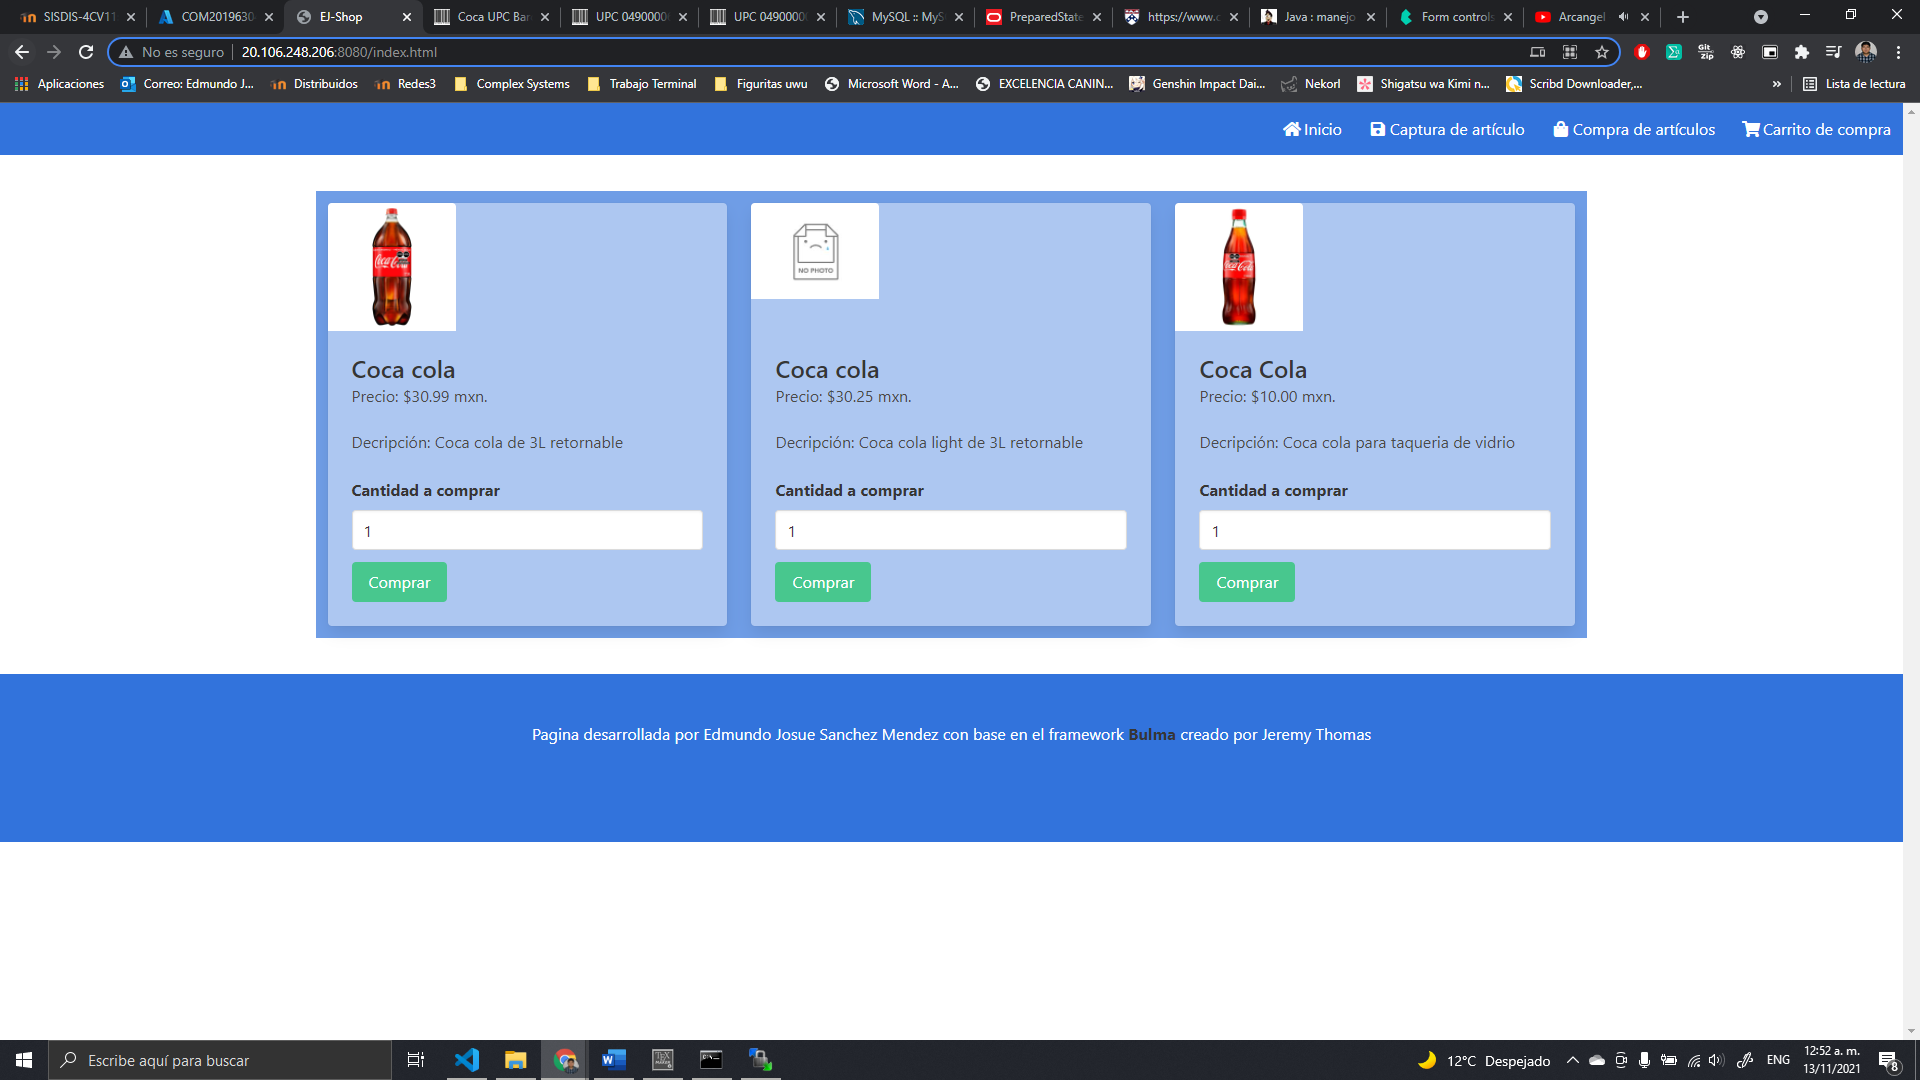
\includegraphics[scale=0.34]{resources/p2.1.2.png}
			\caption{Resultado de la búsqueda de la palabra ``coca''.}\label{fig:picture}
		\end{figure}
		\begin{figure}[H]
			\centering
			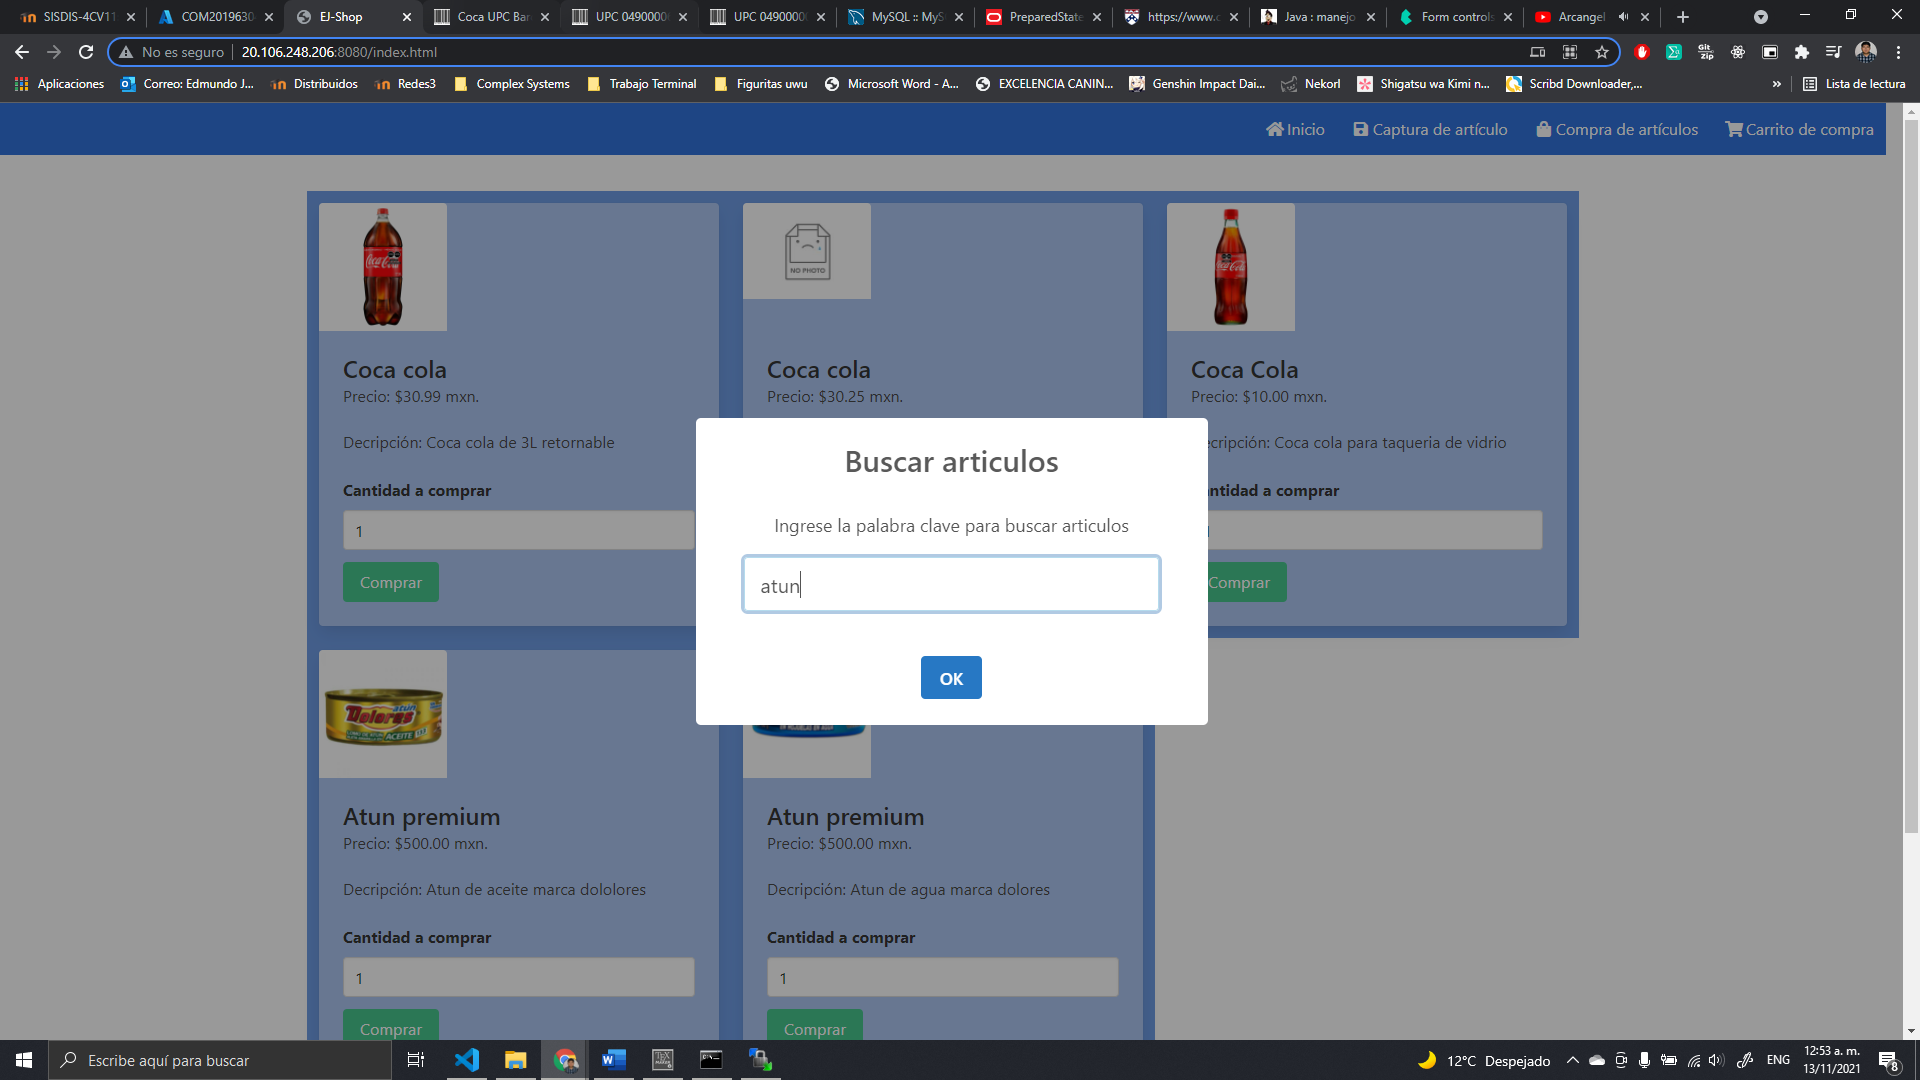
\includegraphics[scale=0.34]{resources/p2.2.1.png}
			\caption{Buscando palabra ``atun''.}\label{fig:picture}
		\end{figure}
		\begin{figure}[H]
			\centering
			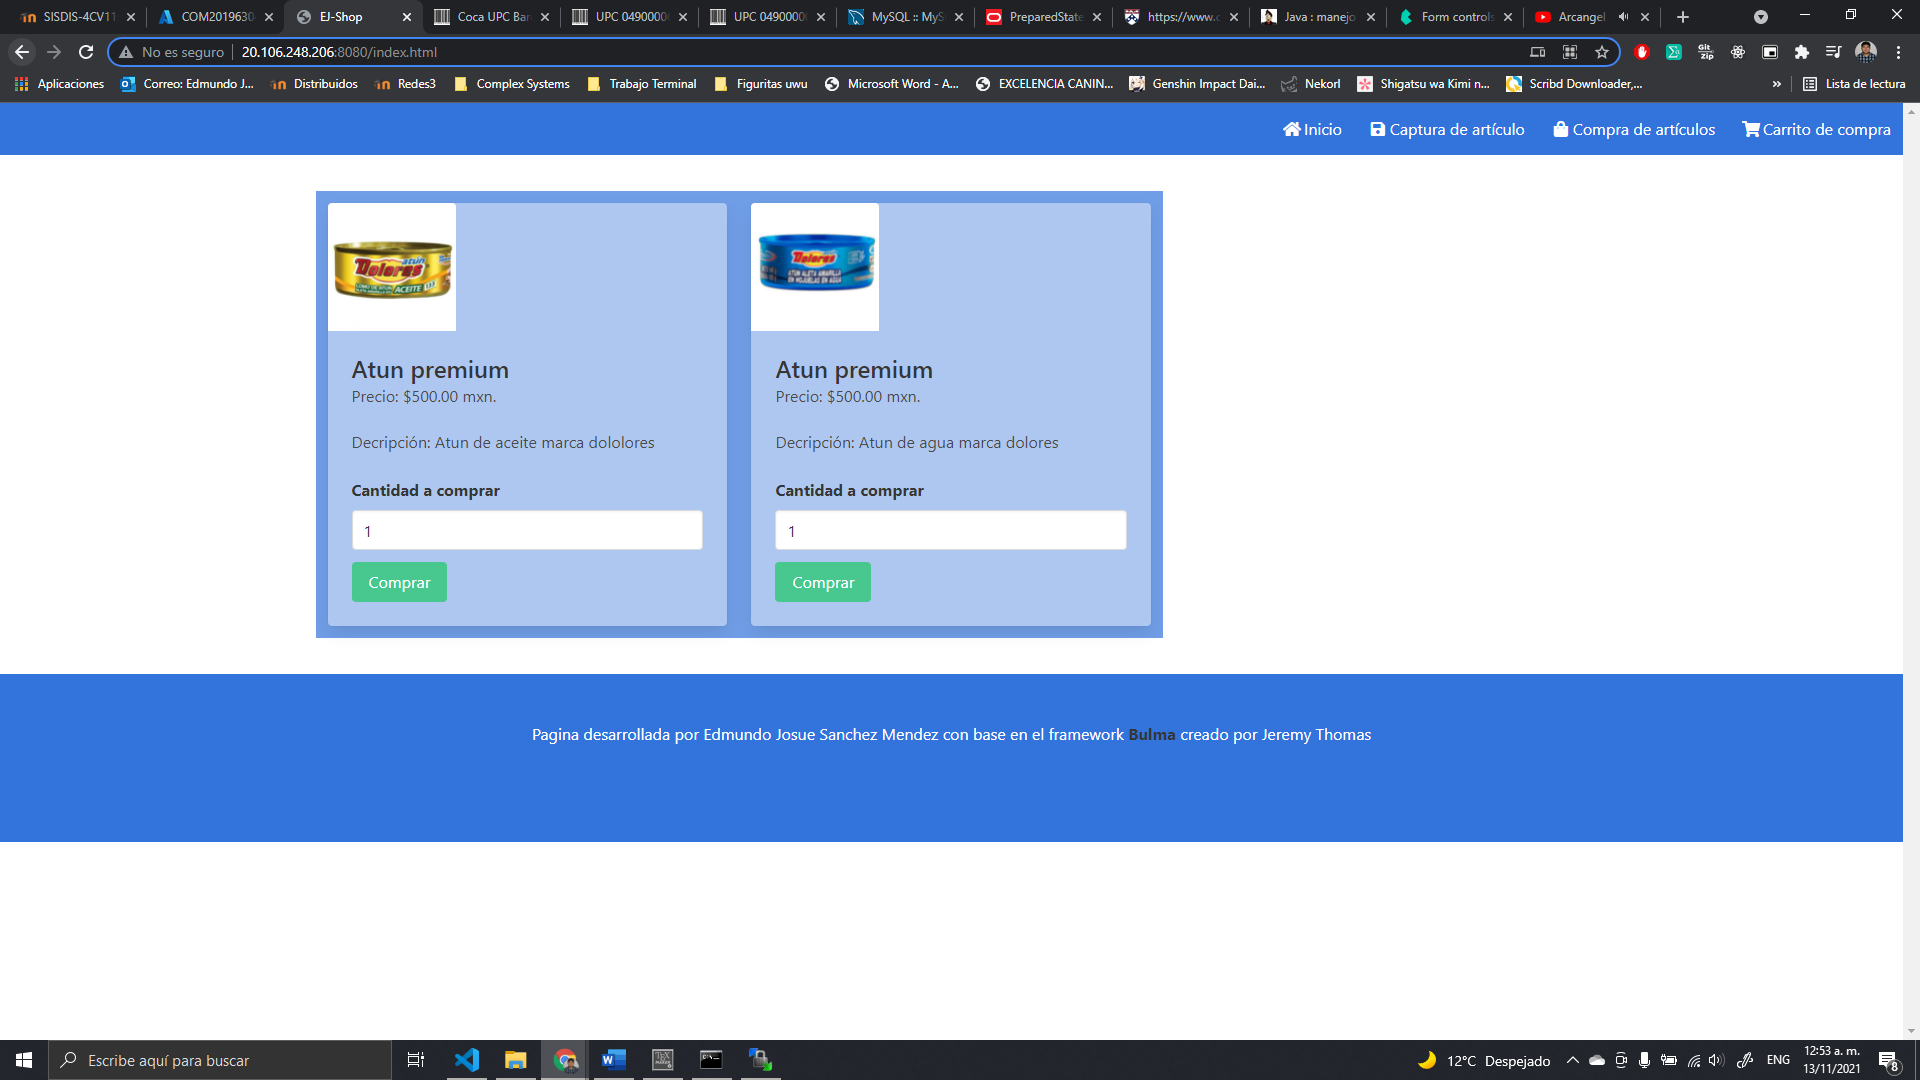
\includegraphics[scale=0.34]{resources/p2.2.2.png}
			\caption{Resultado de la búsqueda de la palabra ``atun''.}\label{fig:picture}
		\end{figure}
		\subsection{Prueba 3. Compra de artículos}
		Recordemos la figura 24 ya que nos sera útil.\par
		La primera prueba sera intentar comprar una cantidad mayor de la que existe en la base de datos, esto en la figura 34 y vemos como en la figura 35 nos sale un error diciendo la cantidad disponible del articulo.
		\begin{figure}[H]
			\centering
			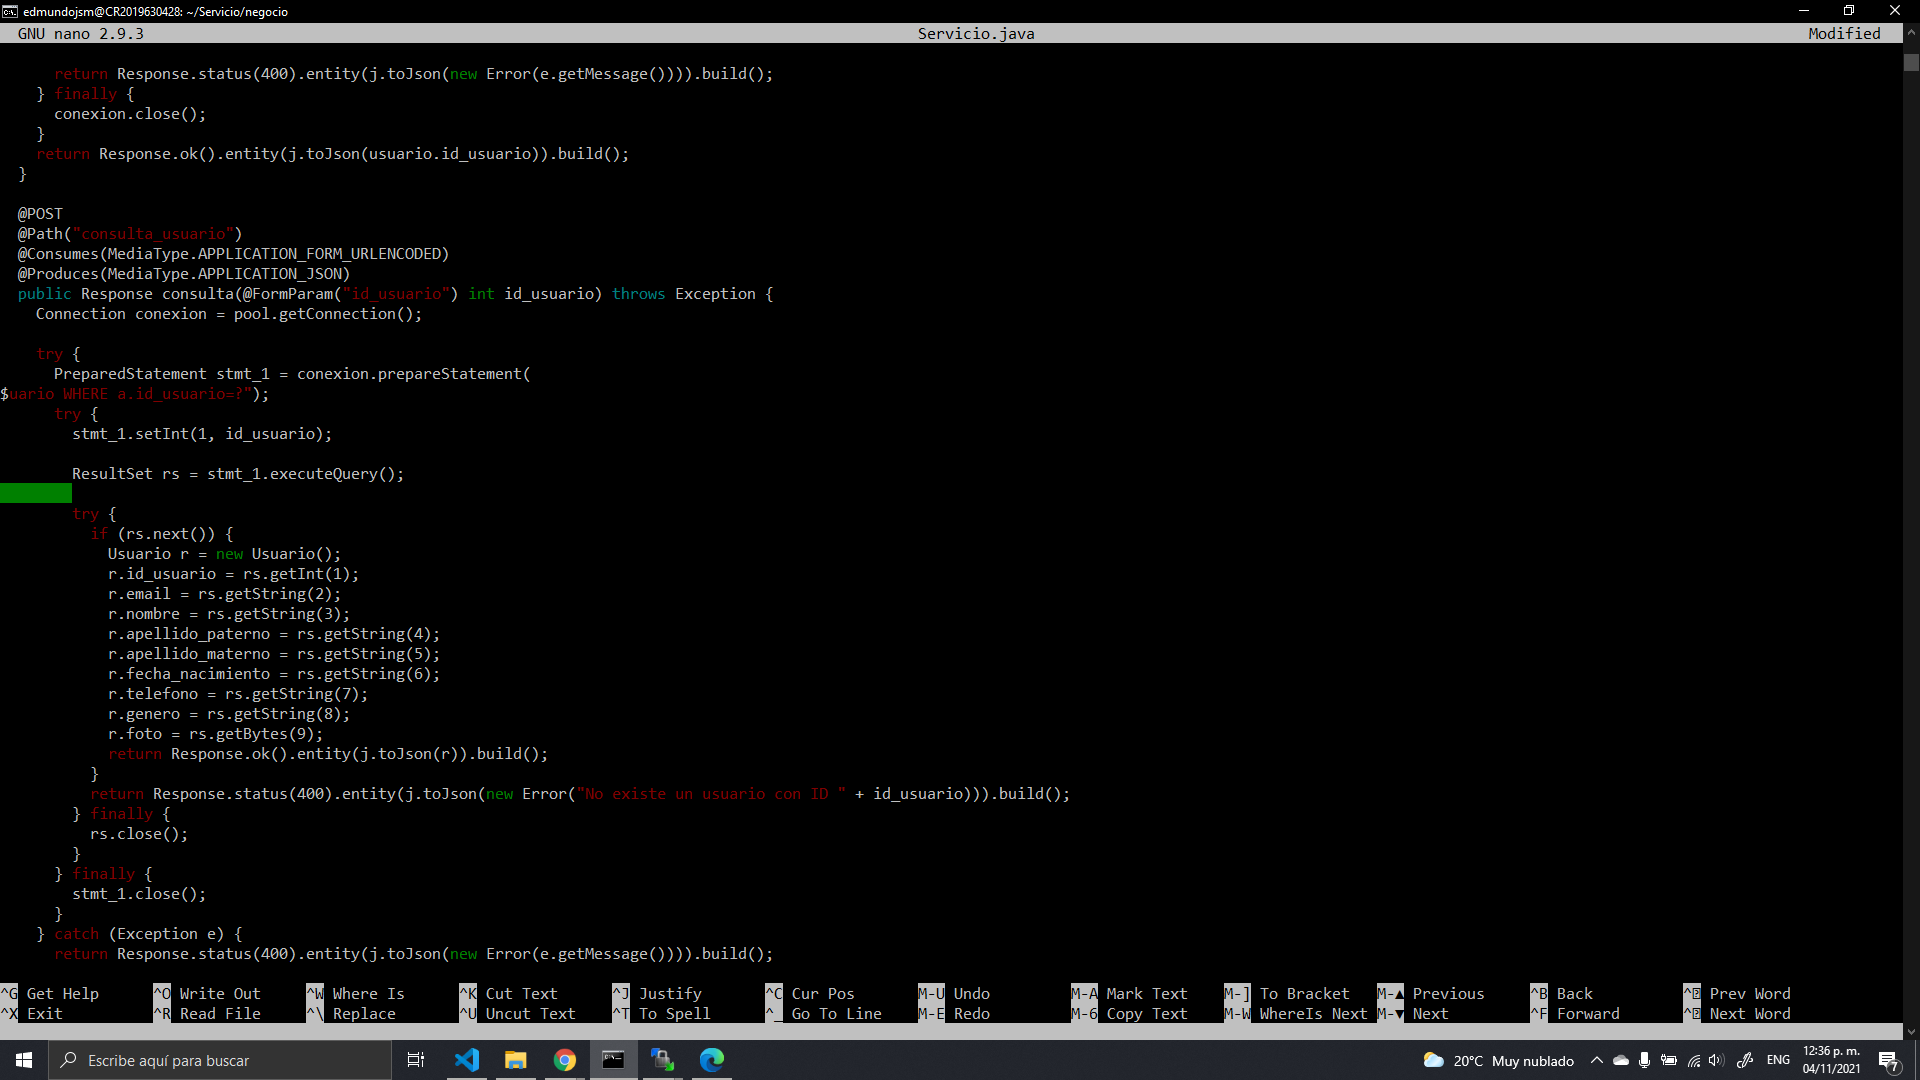
\includegraphics[scale=0.34]{resources/p3.1.png}
			\caption{Intento de comprar una cantidad mayor de la existente.}\label{fig:picture}
		\end{figure}
		\begin{figure}[H]
			\centering
			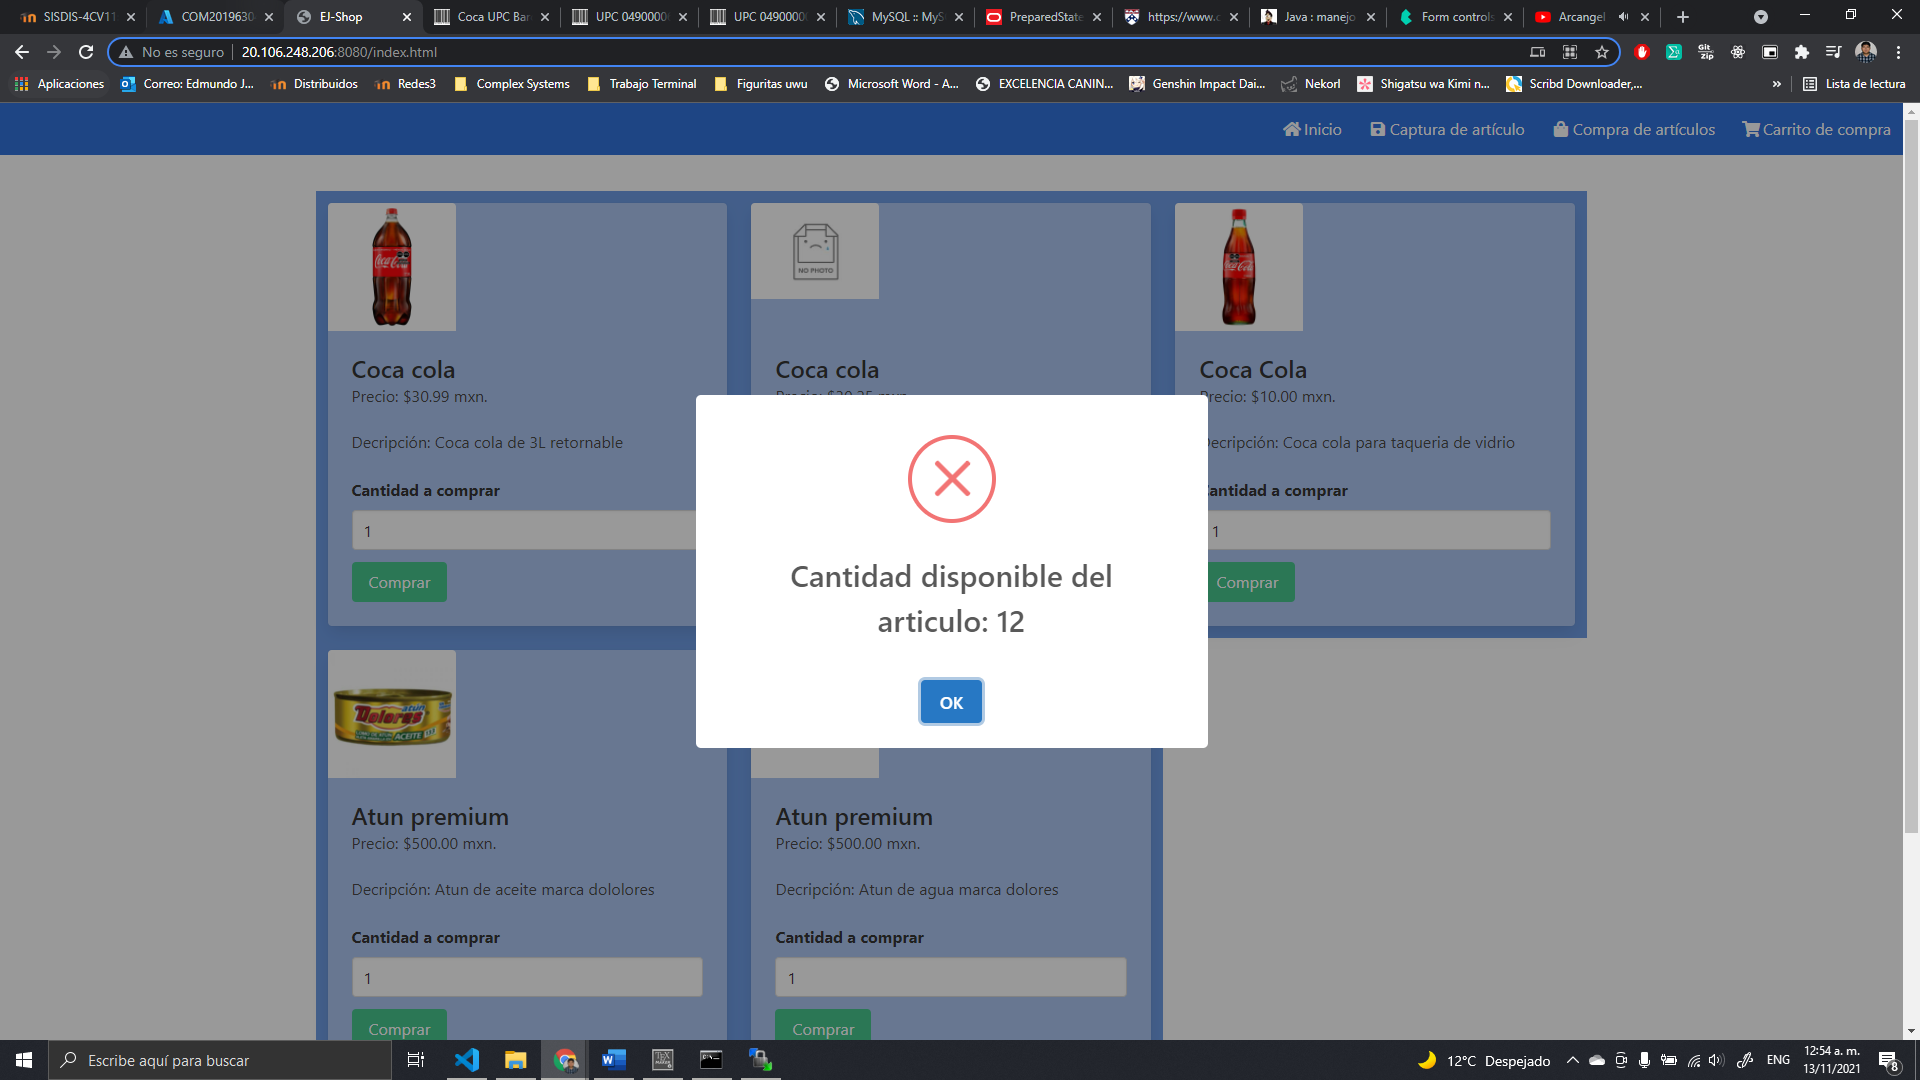
\includegraphics[scale=0.34]{resources/p3.2.png}
			\caption{Error al comprar, ya que no hay suficiente cantidad para cubrir la compra.}\label{fig:picture}
		\end{figure}
		En las siguientes dos figuras vemos como podemos comprar si la cantidad solicitada es menor o igual a la existente
		\begin{figure}[H]
			\centering
			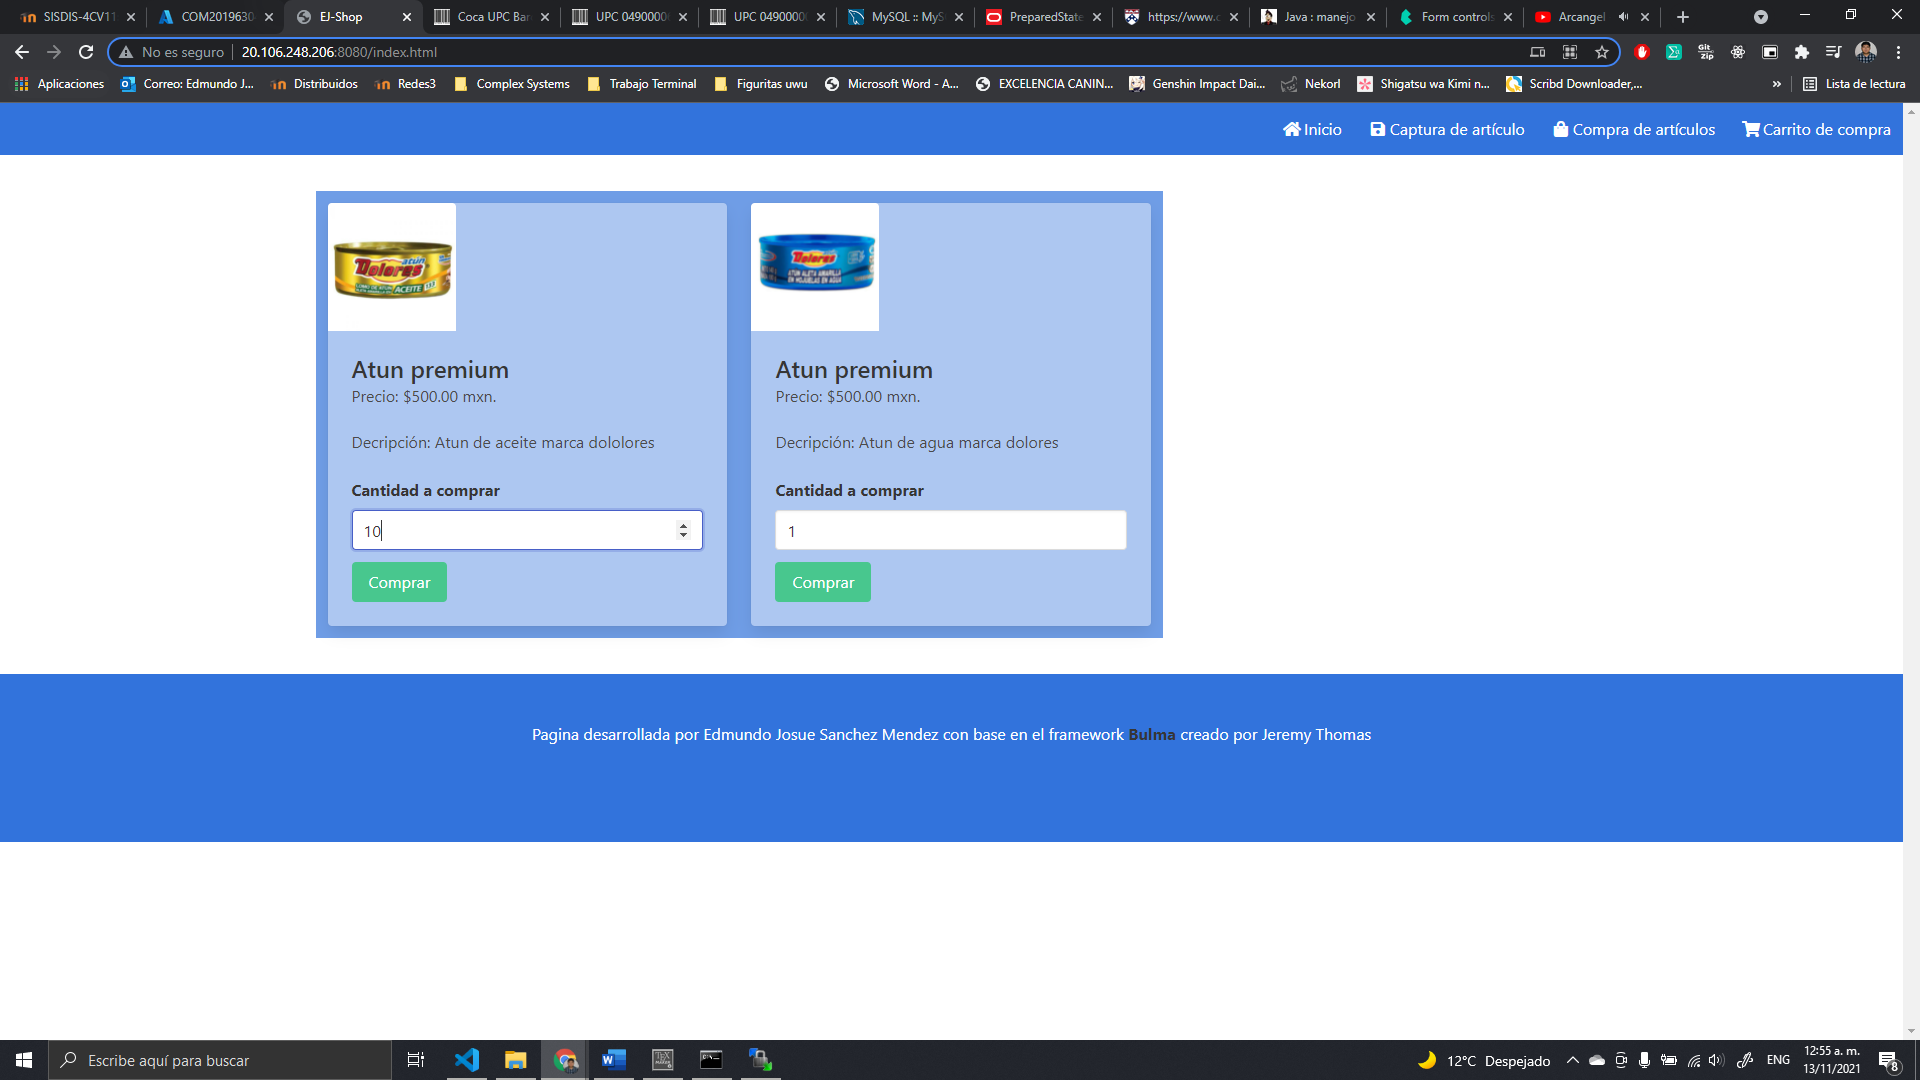
\includegraphics[scale=0.34]{resources/p3.3.png}
			\caption{Cantidad a comprar de 10.}\label{fig:picture}
		\end{figure}
		\begin{figure}[H]
			\centering
			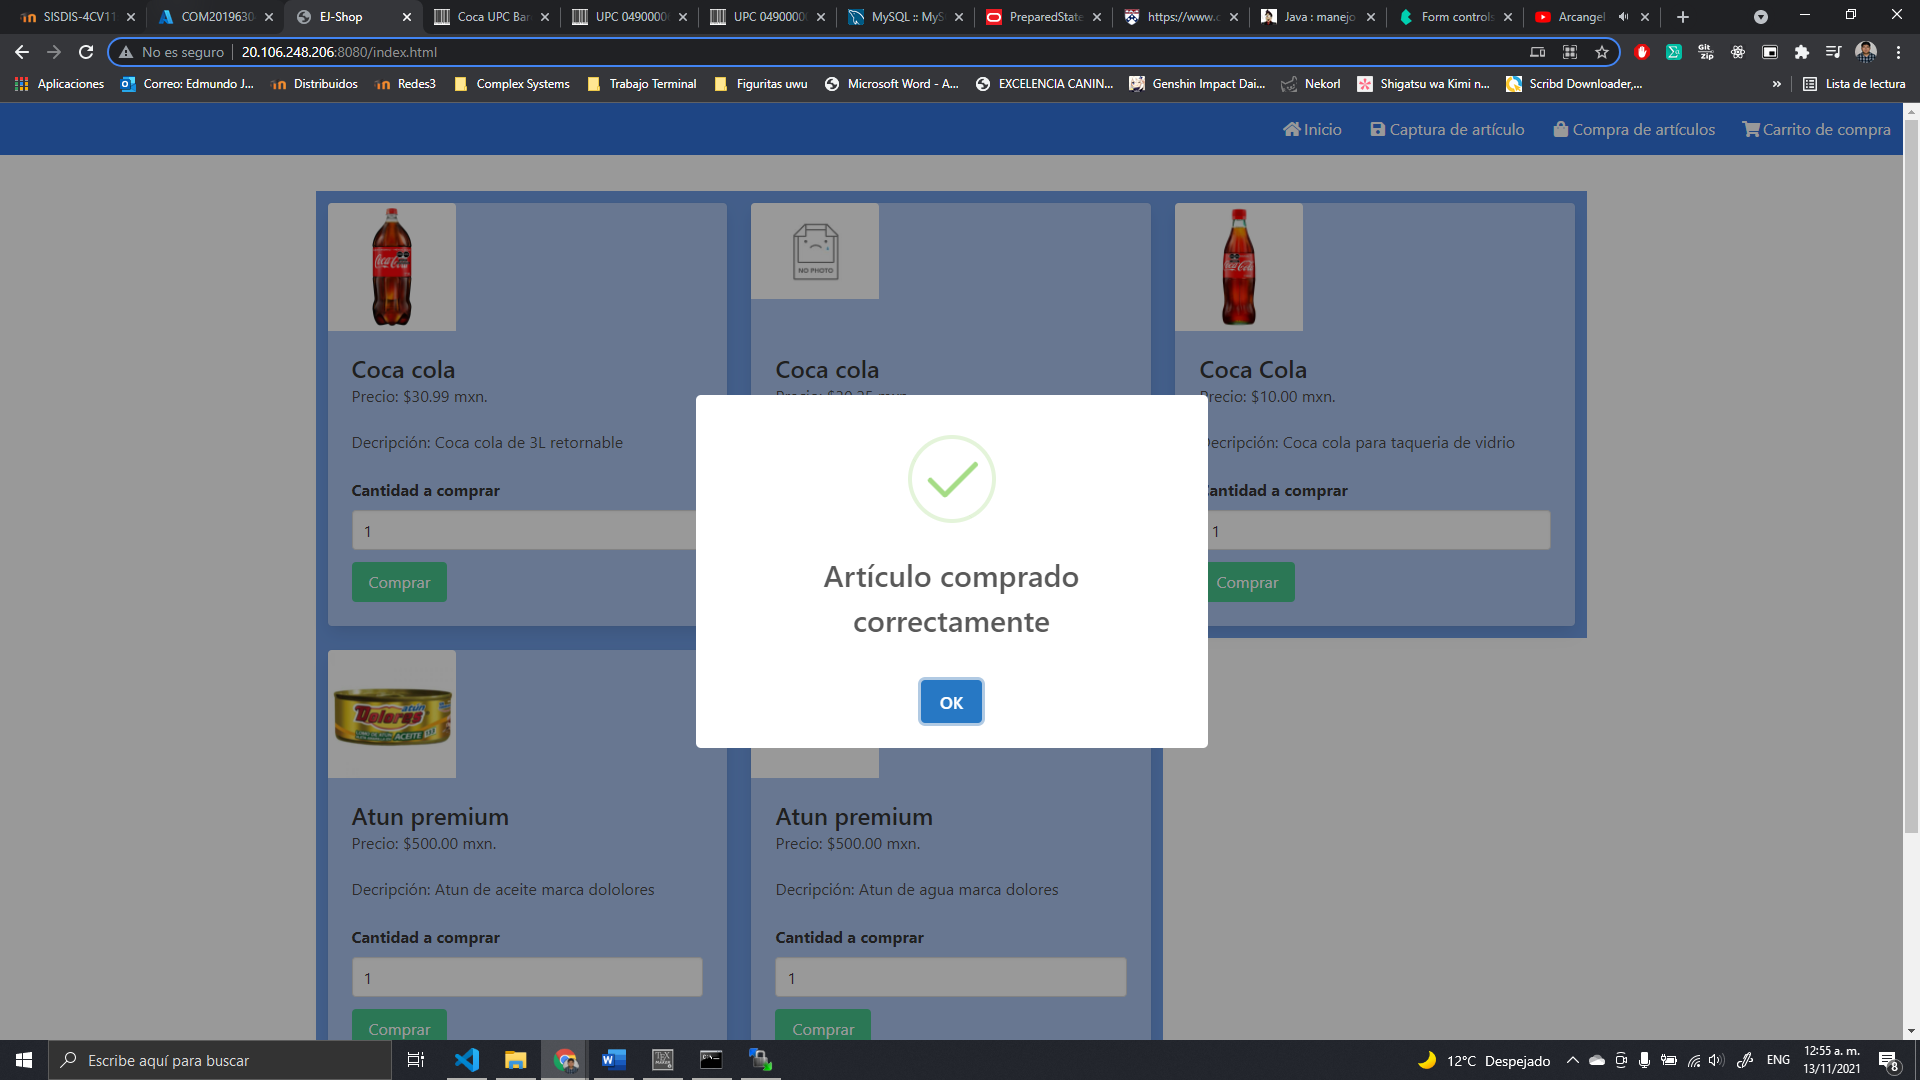
\includegraphics[scale=0.34]{resources/p3.4.png}
			\caption{Compra realizada con éxito.}\label{fig:picture}
		\end{figure}
		Una prueba mas es la que podemos ver en las siguientes 2 figuras comprando directamente de la pagina de inicio, esto para poder ver que la funcionalidad de compra también esta disponible en esta opción, sin embargo, hay un pequeño detalle y es que podemos comprar varias veces un mismo articulo siempre y cuando podamos cubrir la cantidad solicitada, es por eso que se realiza esta prueba.
		\begin{figure}[H]
			\centering
			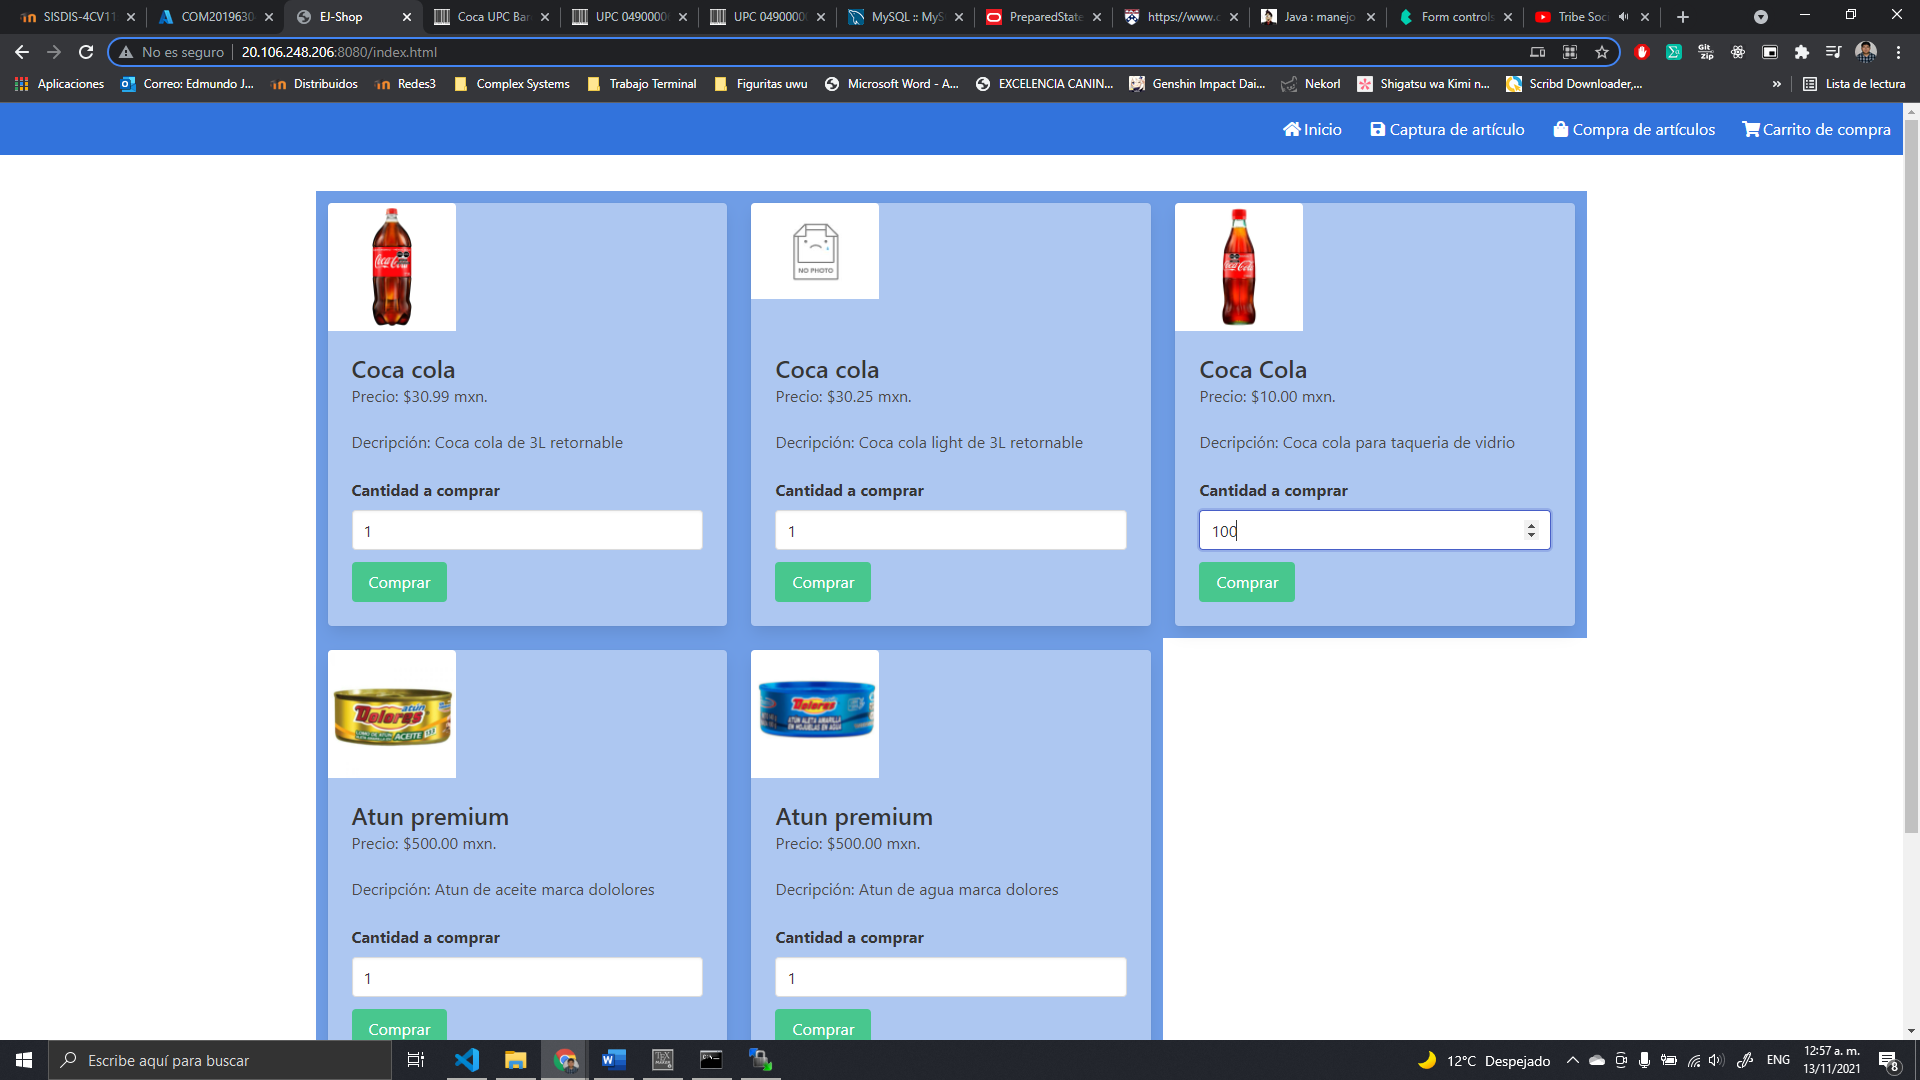
\includegraphics[scale=0.34]{resources/p3.6_recompra.png}
			\caption{Re compra de un articulo.}\label{fig:picture}
		\end{figure}
		\begin{figure}[H]
			\centering
			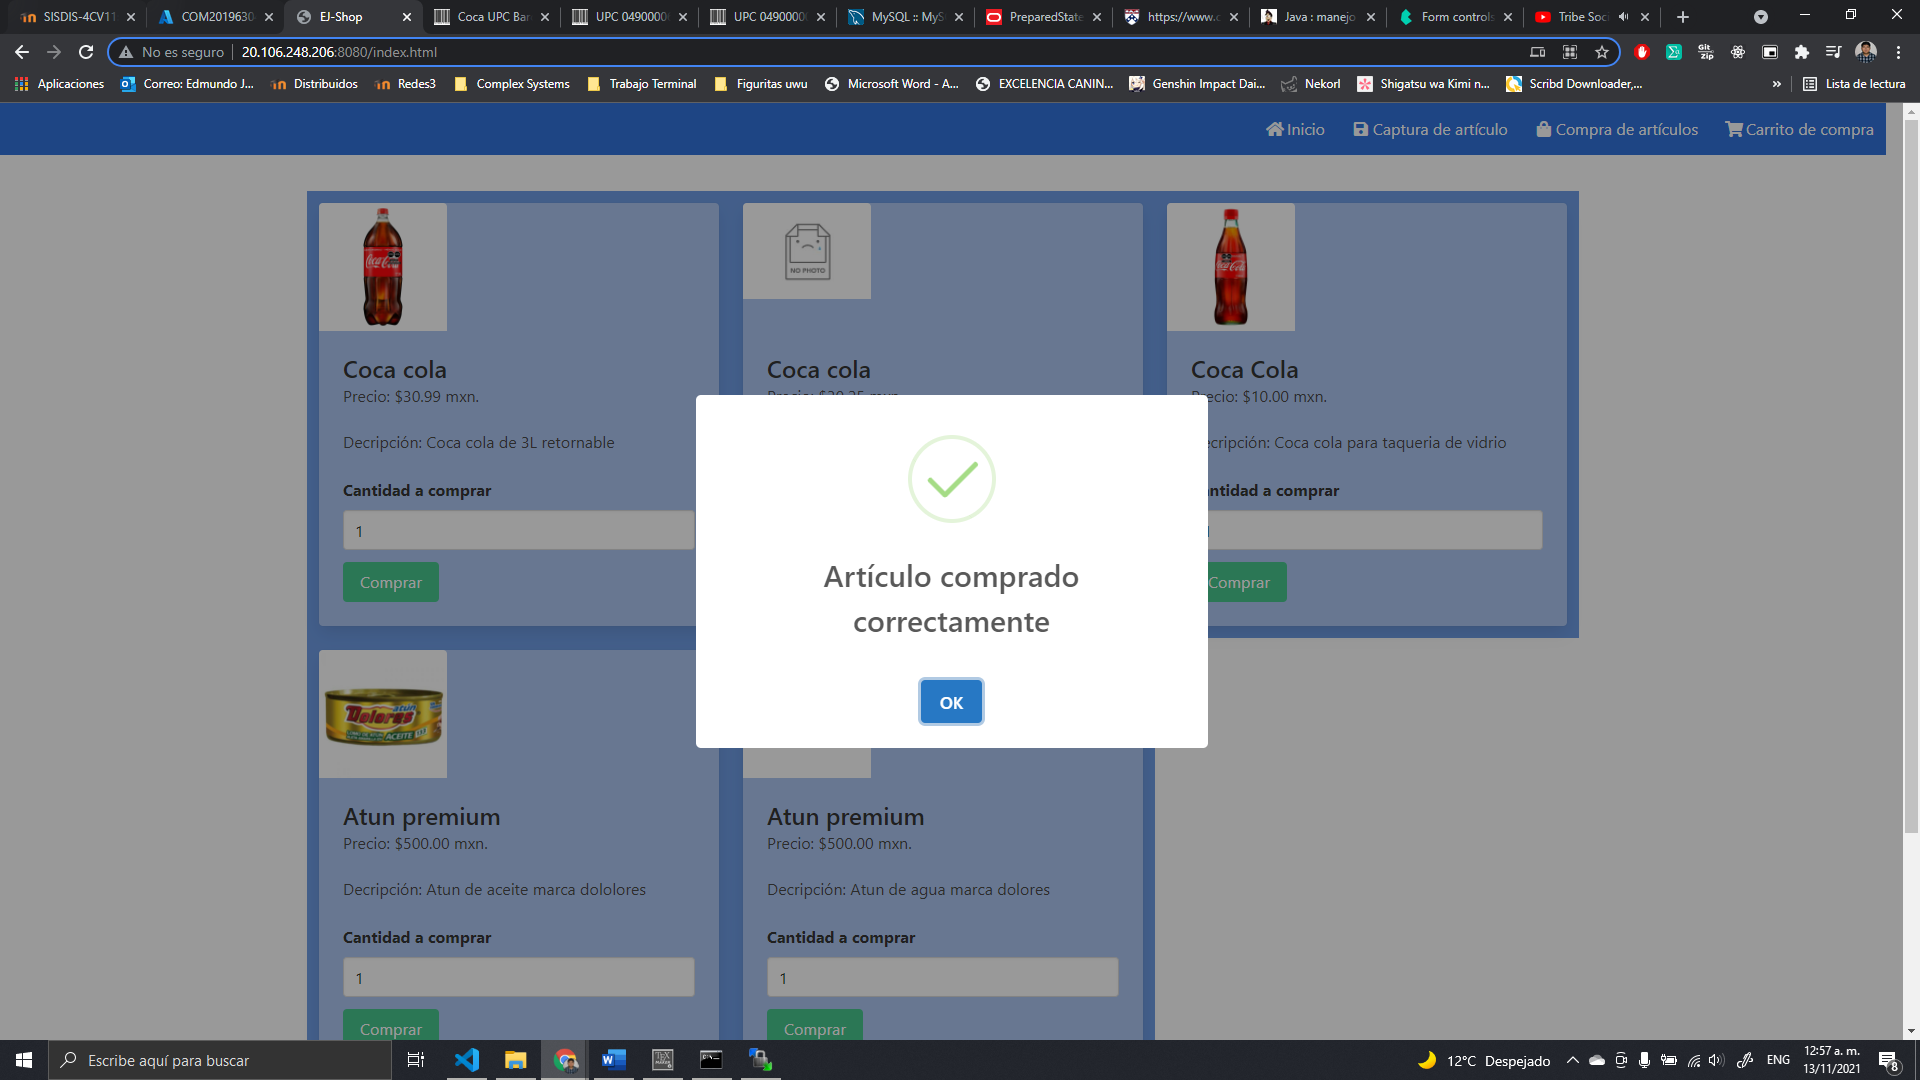
\includegraphics[scale=0.34]{resources/p3.7_recompra.png}
			\caption{Re compra de un articulo realizada con éxito.}\label{fig:picture}
		\end{figure}
		Y como podemos ver en la figura 40 la base de datos se fue actualizando con base en al compras realizadas, tanto en la tabla de artículos como en la tabla de carrito\_compra.
		\begin{figure}[H]
			\centering
			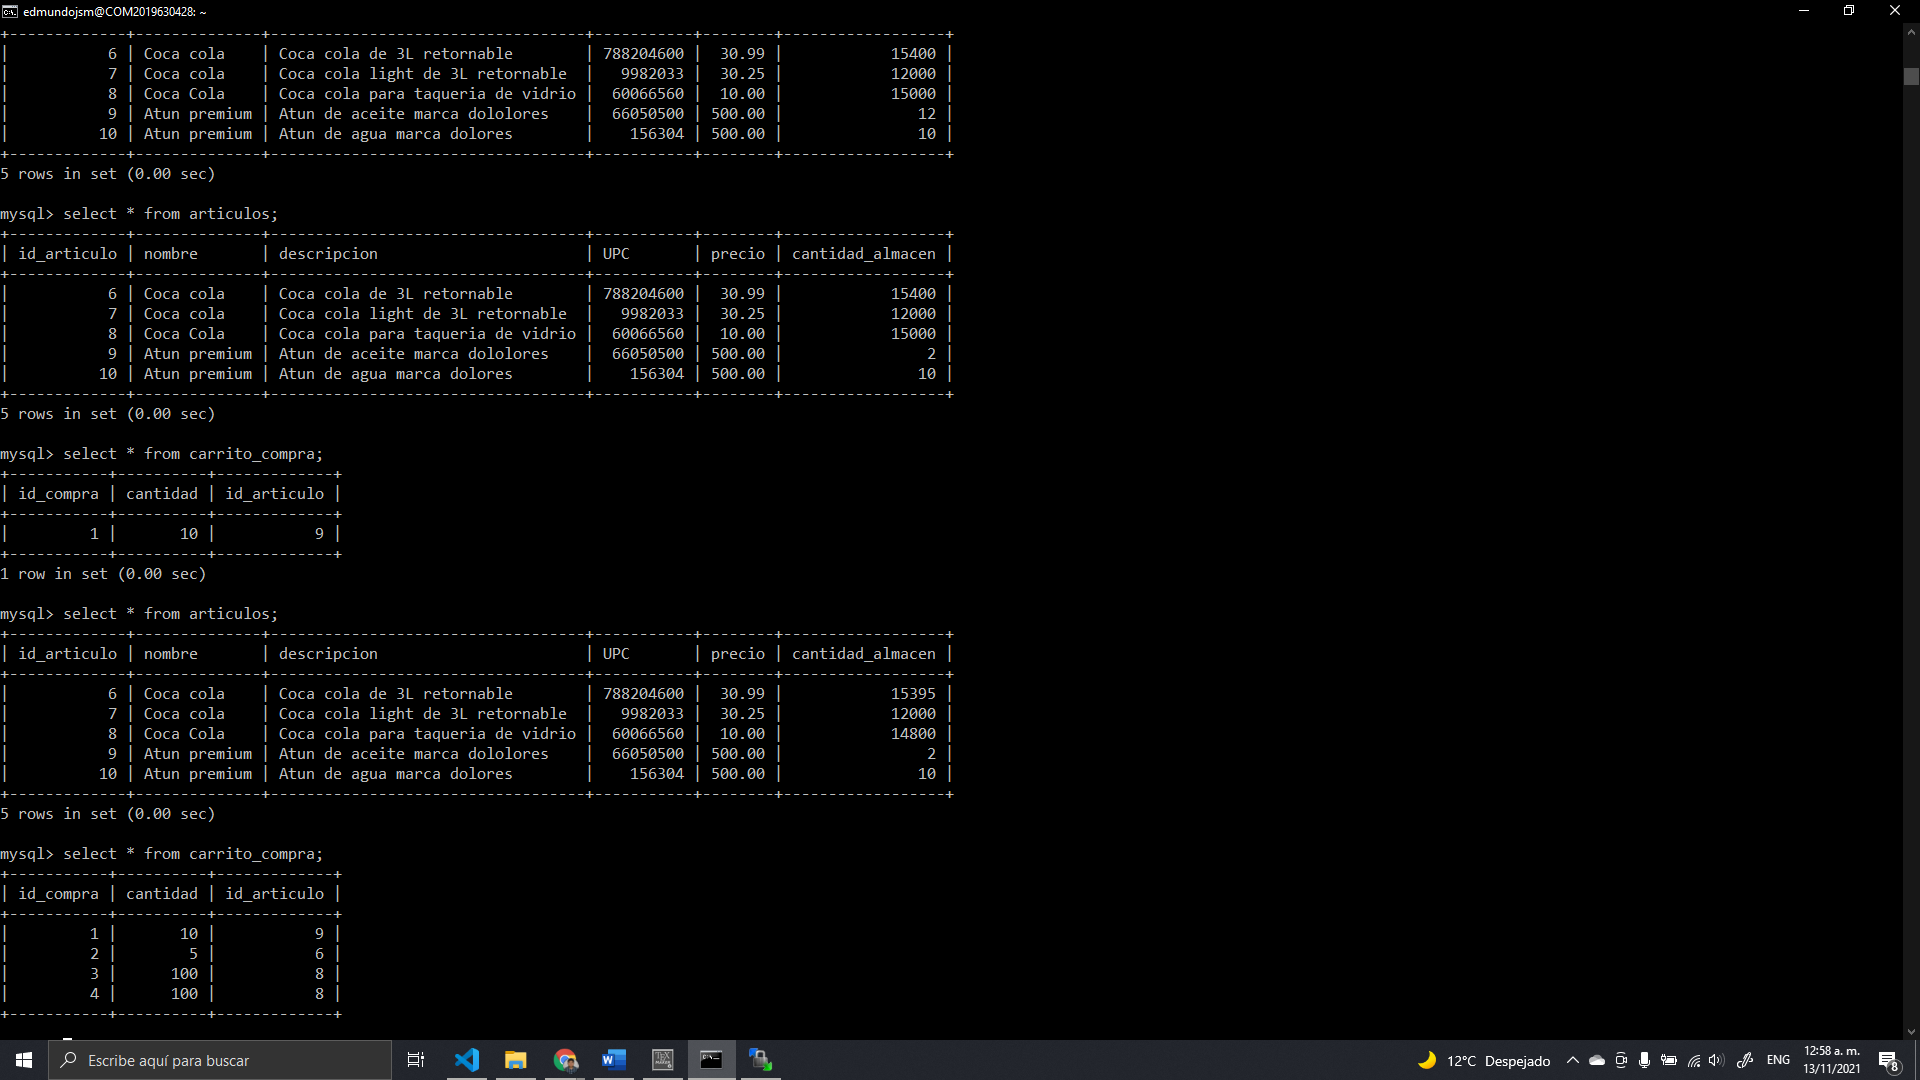
\includegraphics[scale=0.34]{resources/bdp3.png}
			\caption{Re compra de un articulo realizada con éxito.}\label{fig:picture}
		\end{figure}
		Ahora en las siguientes tres imágenes veremos la prueba de compra desde el celular junto con la opción de búsqueda de articulo.
		\begin{figure}[H]
			\centering
			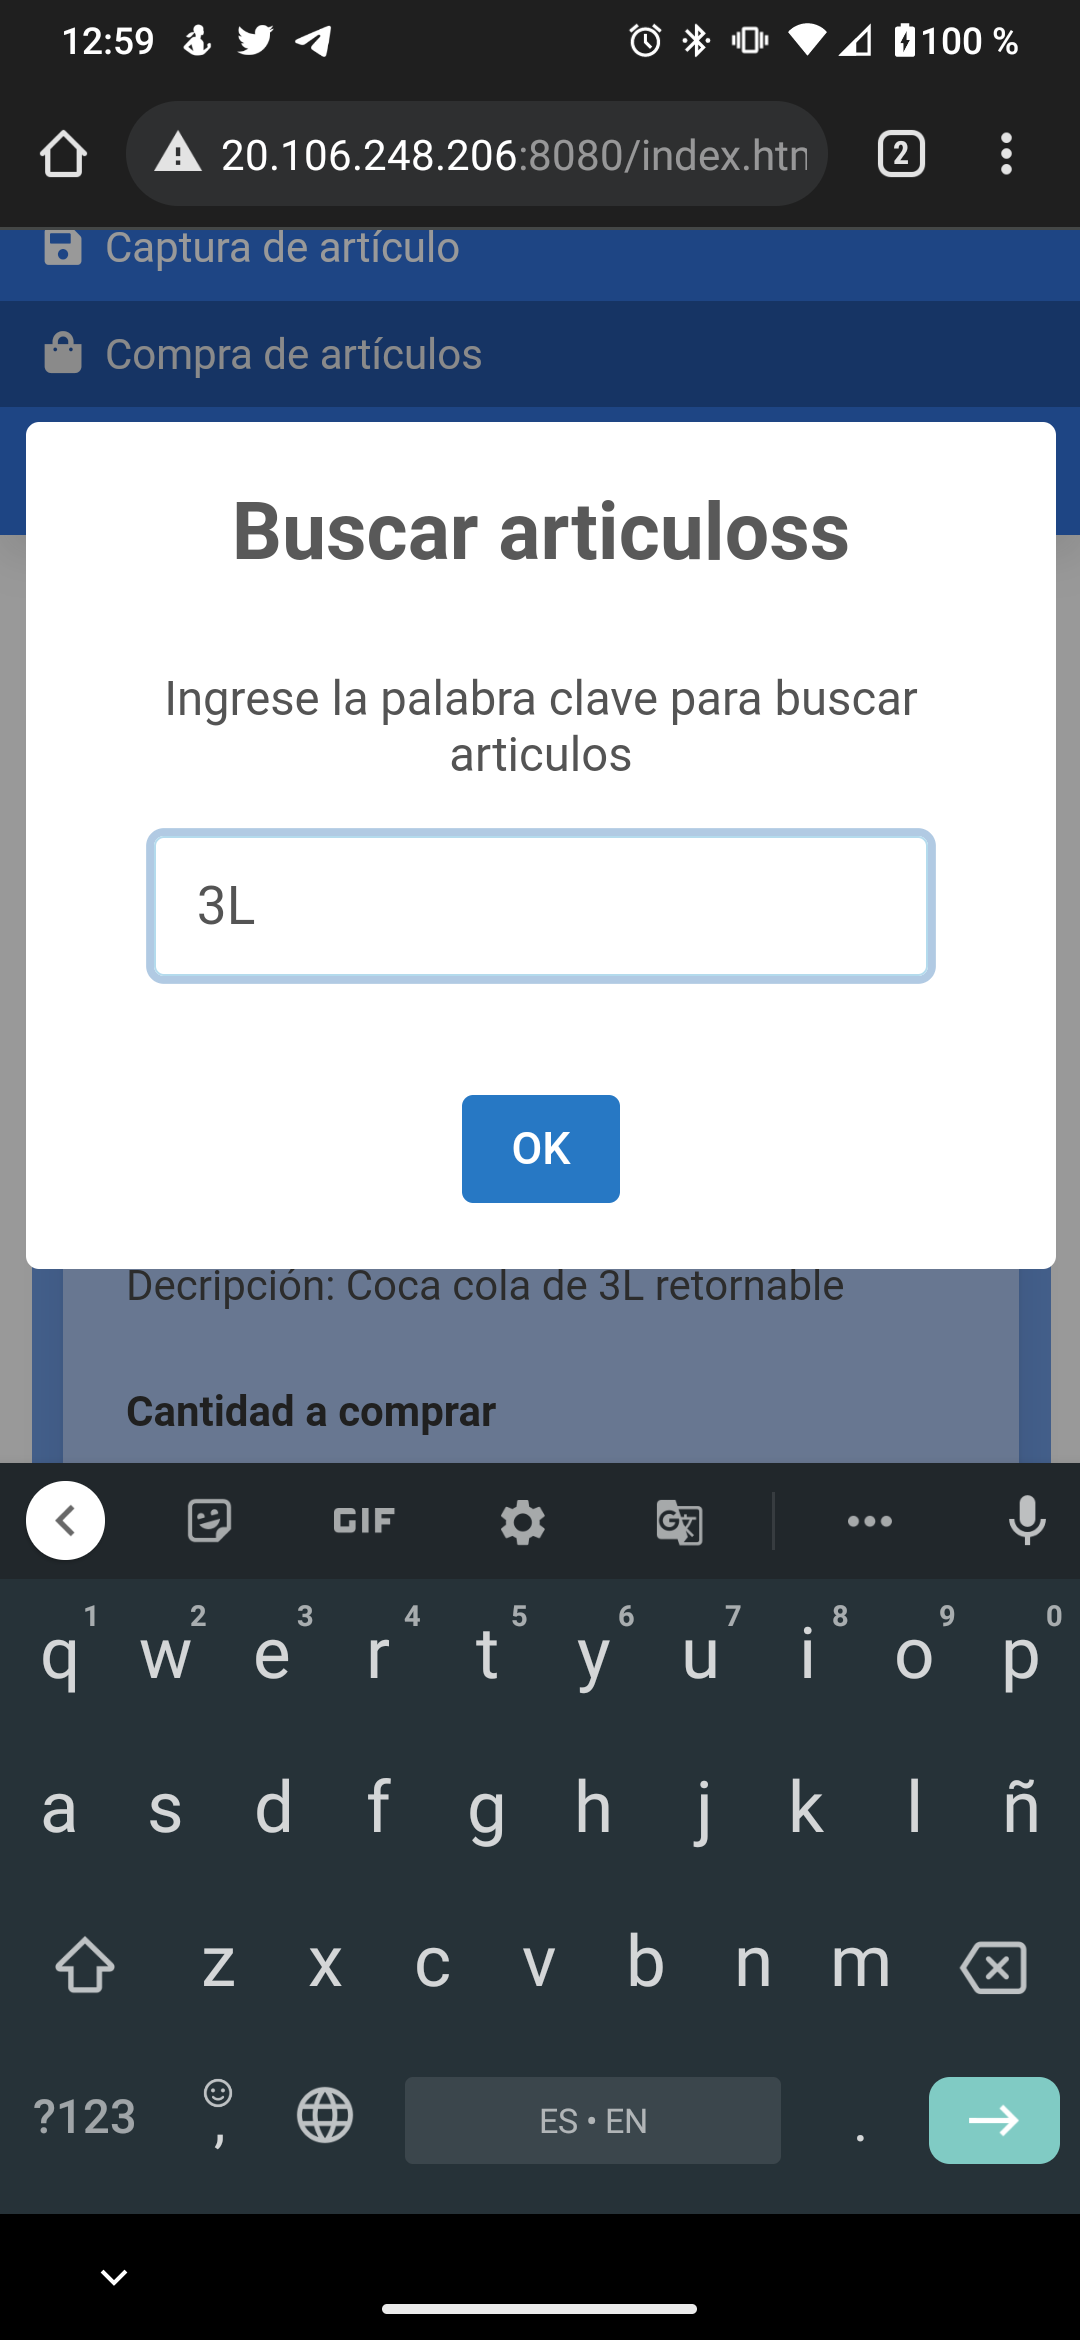
\includegraphics[scale=0.27]{resources/Screenshot_20211113-005920.png}
			\caption{Busqueda de articulos con la palabra 3L.}\label{fig:picture}
		\end{figure}
		\begin{figure}[H]
			\centering
			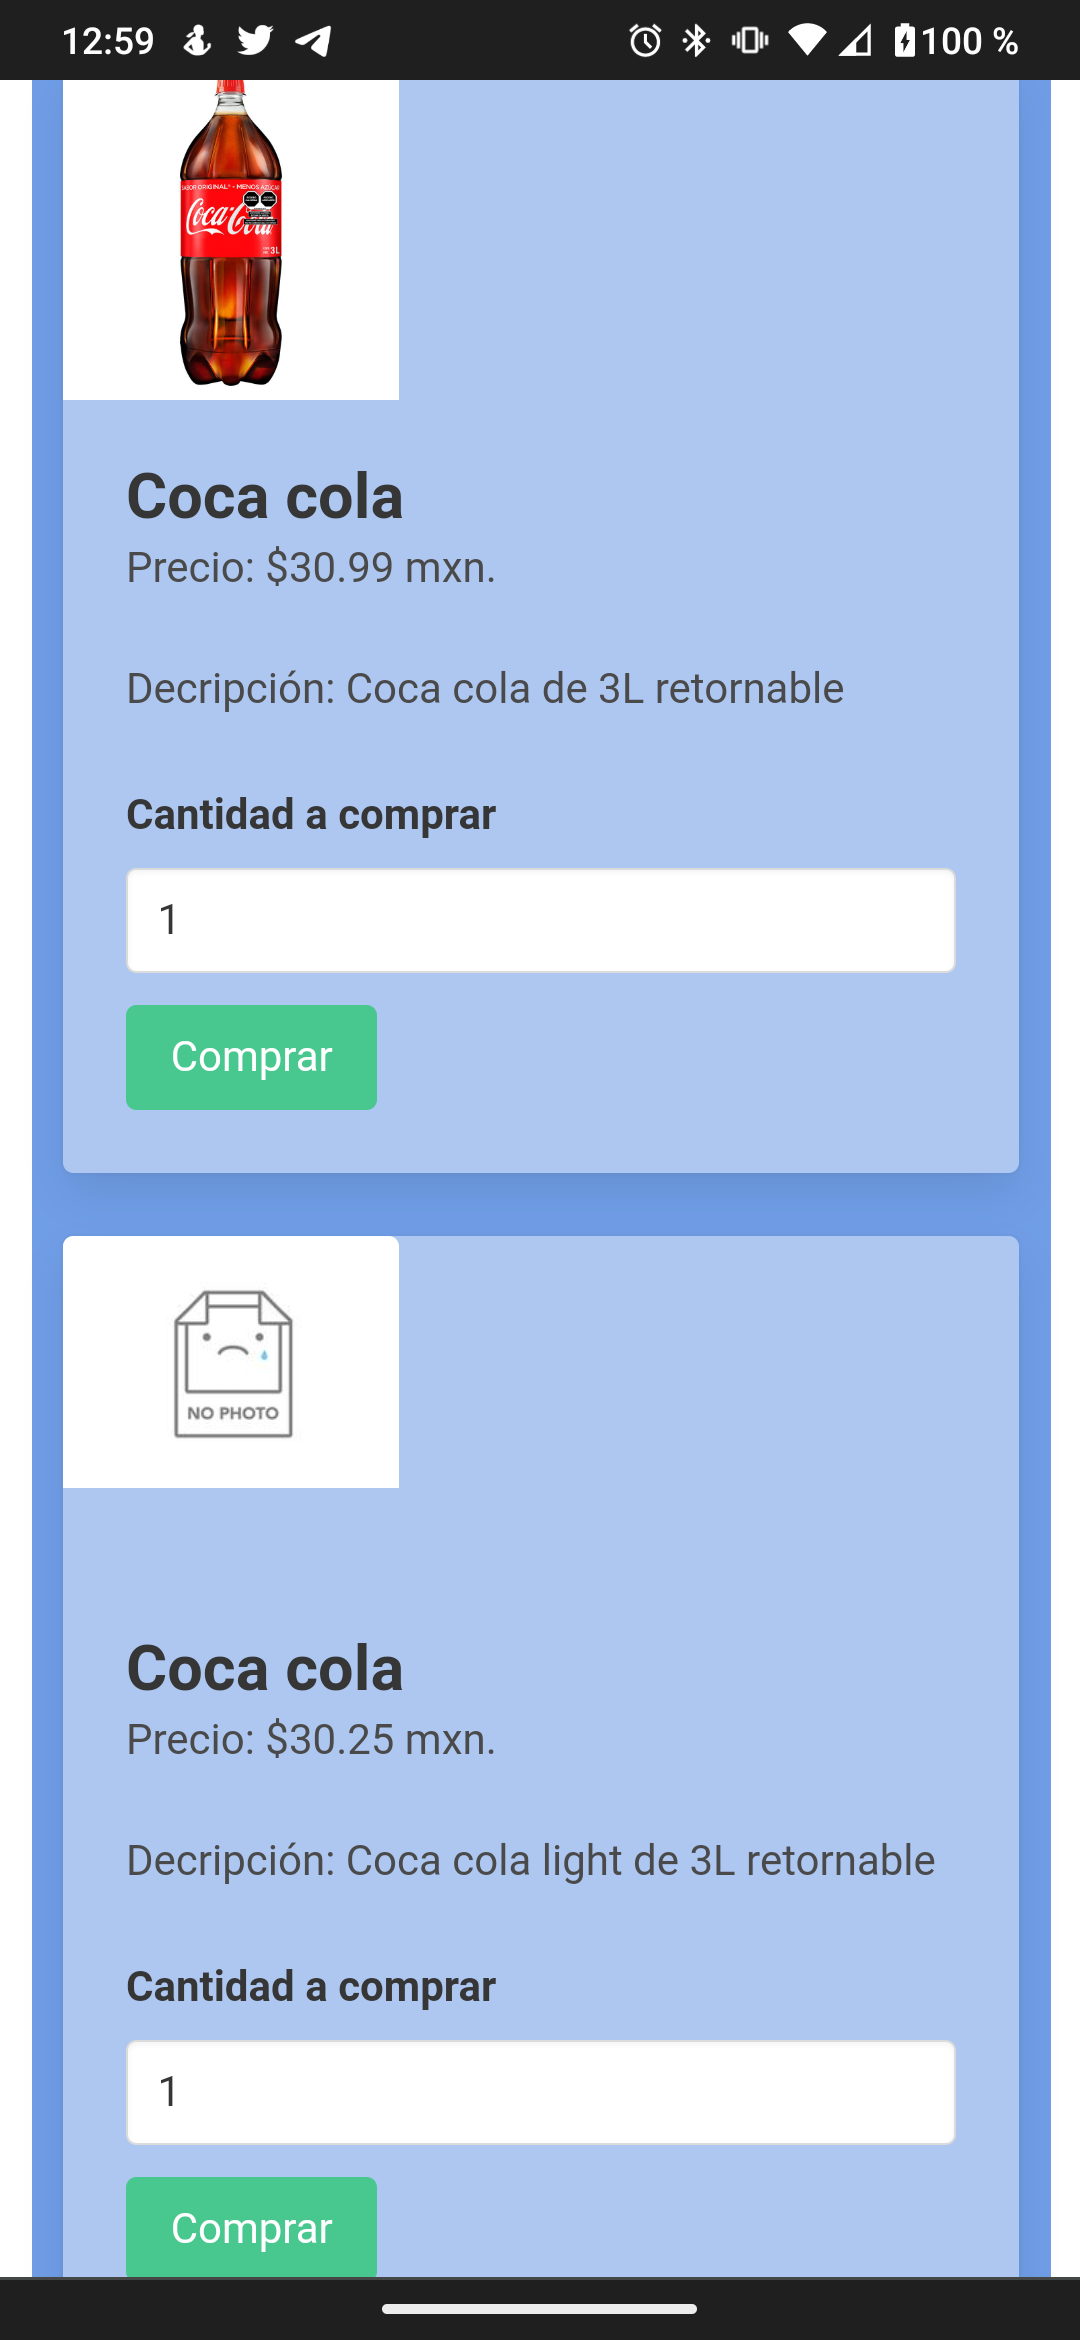
\includegraphics[scale=0.27]{resources/Screenshot_20211113-005930.png}
			\caption{Desplegado de los artículos.}\label{fig:picture}
		\end{figure}
		\begin{figure}[H]
			\centering
			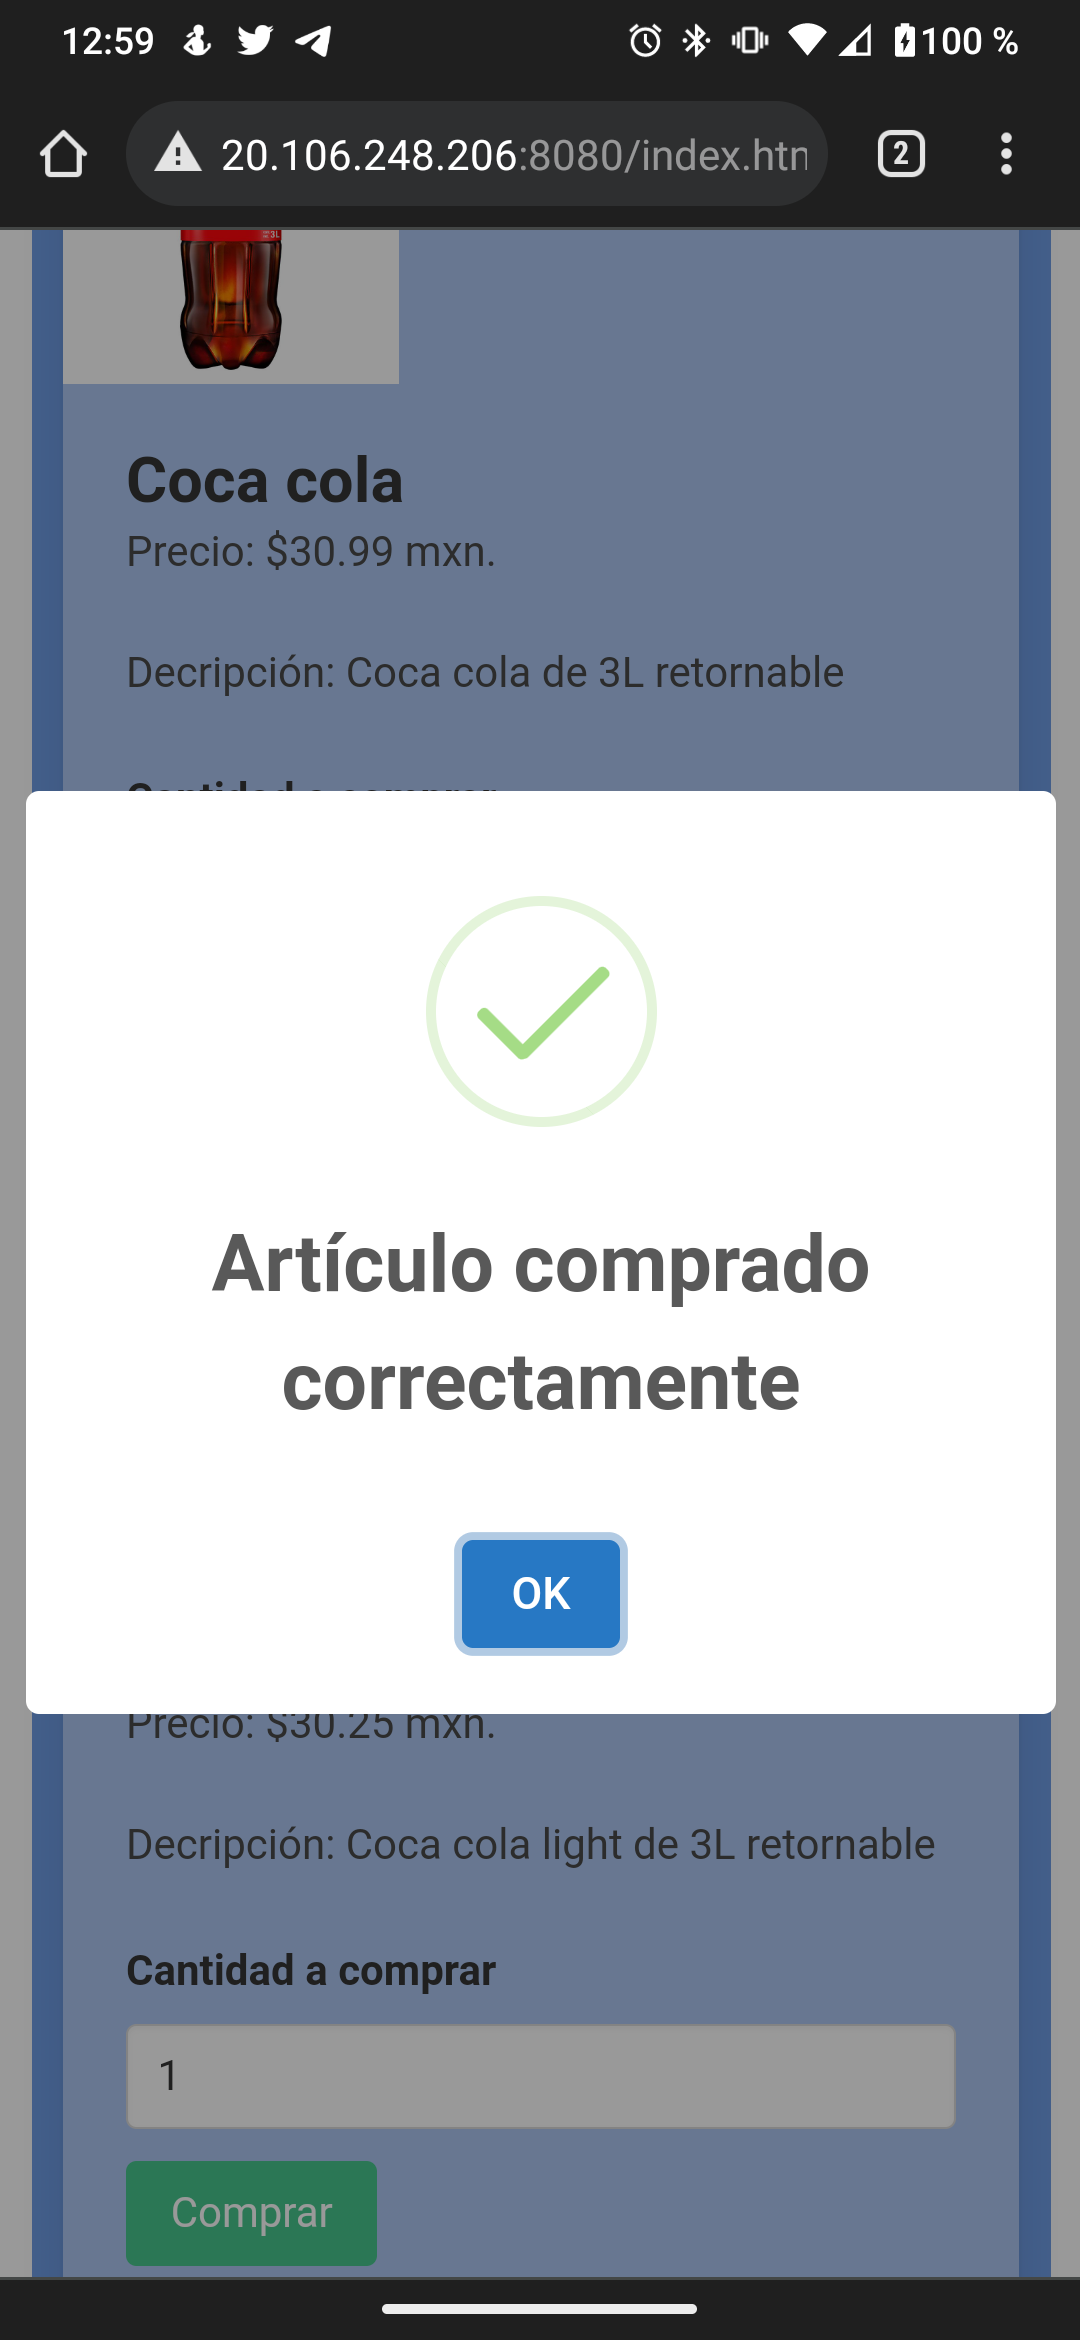
\includegraphics[scale=0.27]{resources/Screenshot_20211113-005957.png}
			\caption{Compra realizada con exitoso.}\label{fig:picture}
		\end{figure}
		Y como podemos ver en la figura 44 la base de datos se fue actualizando con base en al compras realizadas, tanto en la tabla de artículos como en la tabla de carrito\_compra.
		\begin{figure}[H]
			\centering
			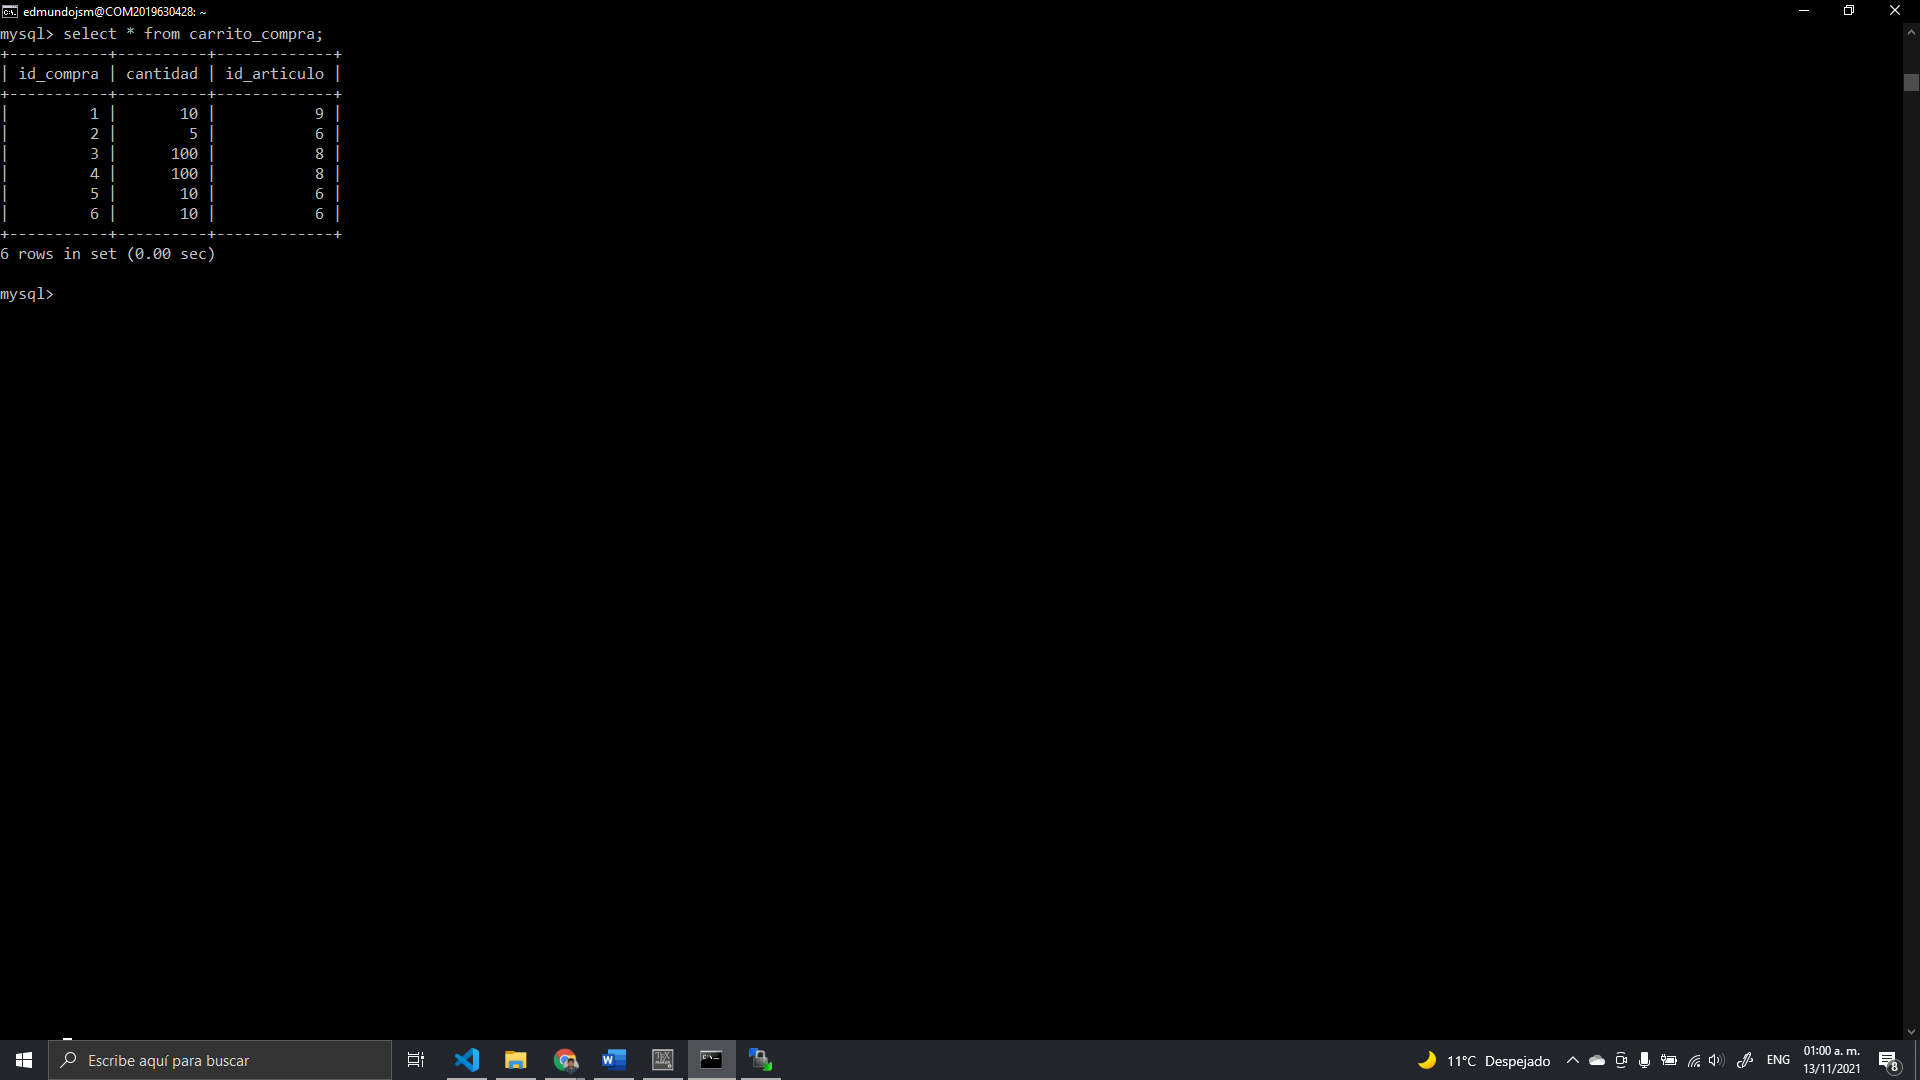
\includegraphics[scale=0.34]{resources/bdp3.1.png}
			\caption{Base de datos actualizada.}\label{fig:picture}
		\end{figure}
		Ahora en las siguientes 3 figuras veamos una vez el intento de compra de mas articulos de los disponibles, como vemos en la base de datos no hay cambio alguno.
		\begin{figure}[H]
			\centering
			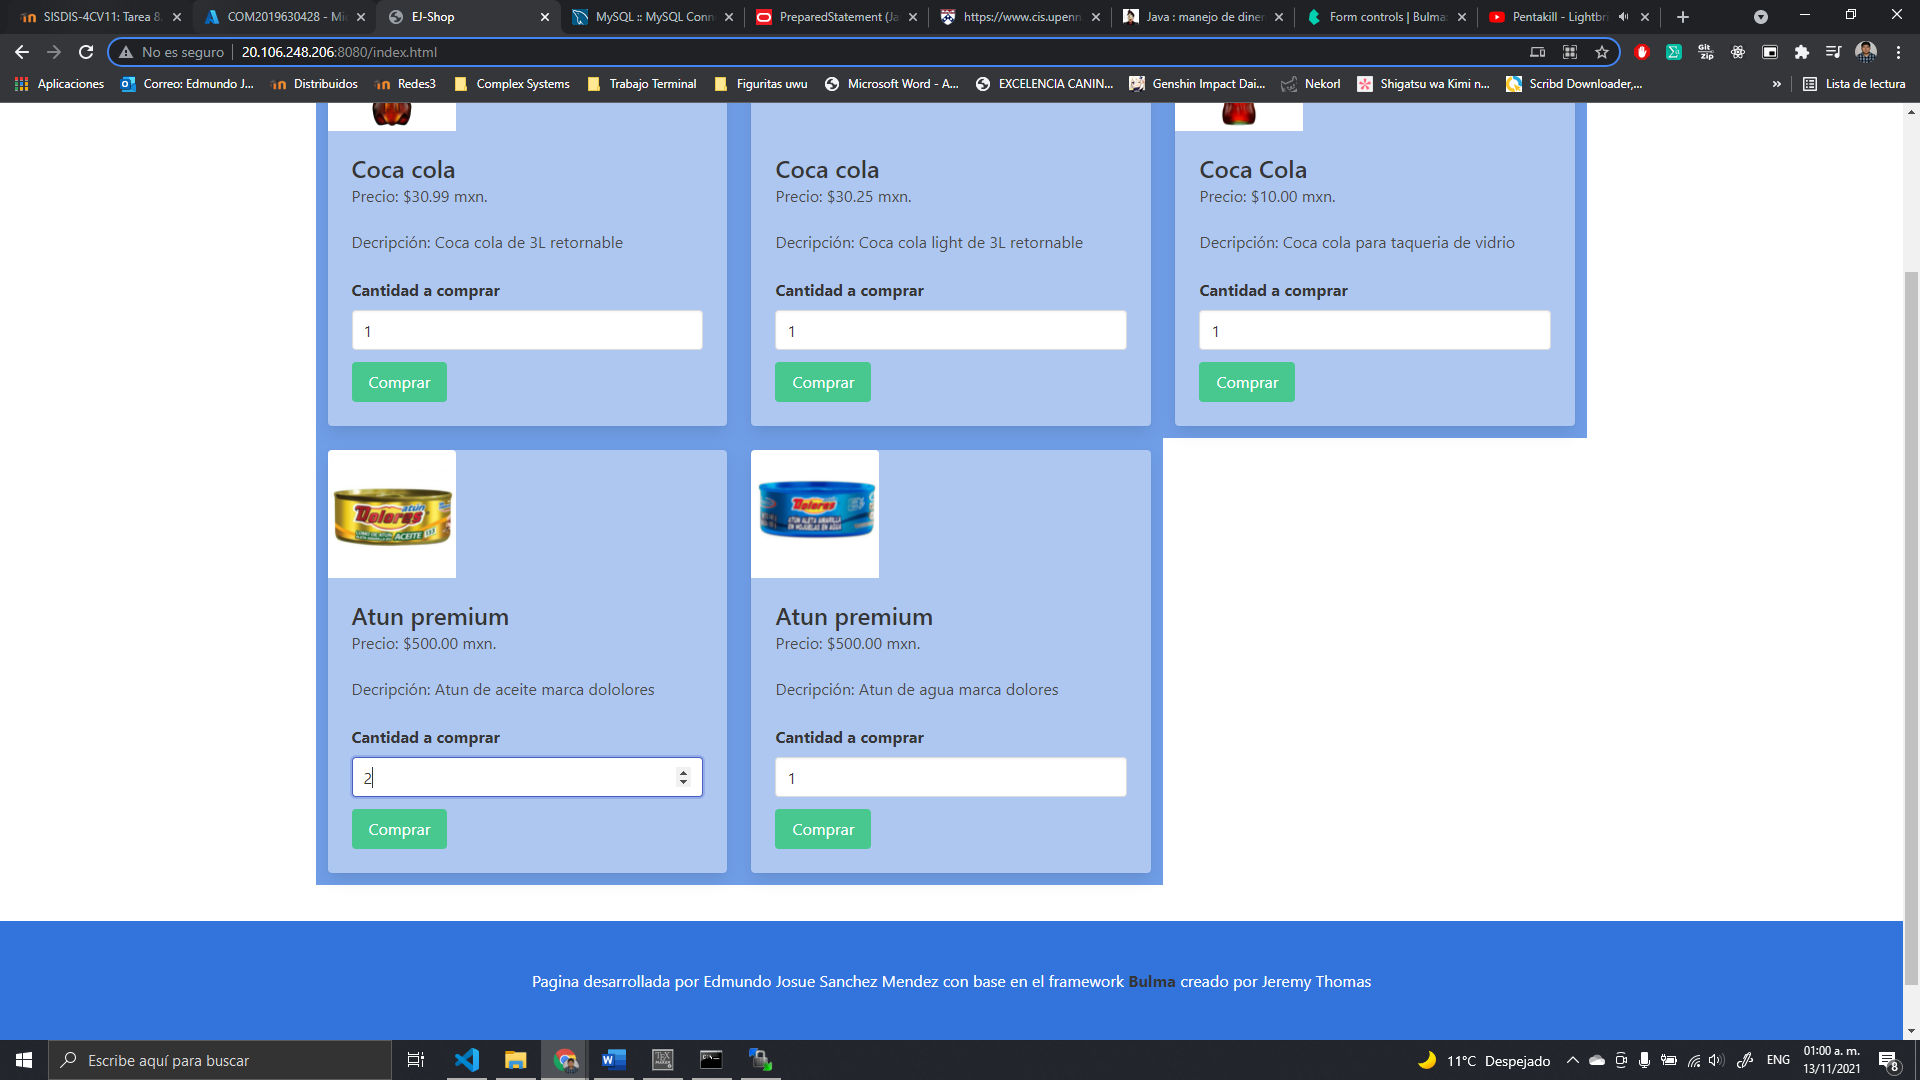
\includegraphics[scale=0.34]{resources/p3mas.png}
			\caption{Intento de compra de mas producto.}\label{fig:picture}
		\end{figure}
		\begin{figure}[H]
			\centering
			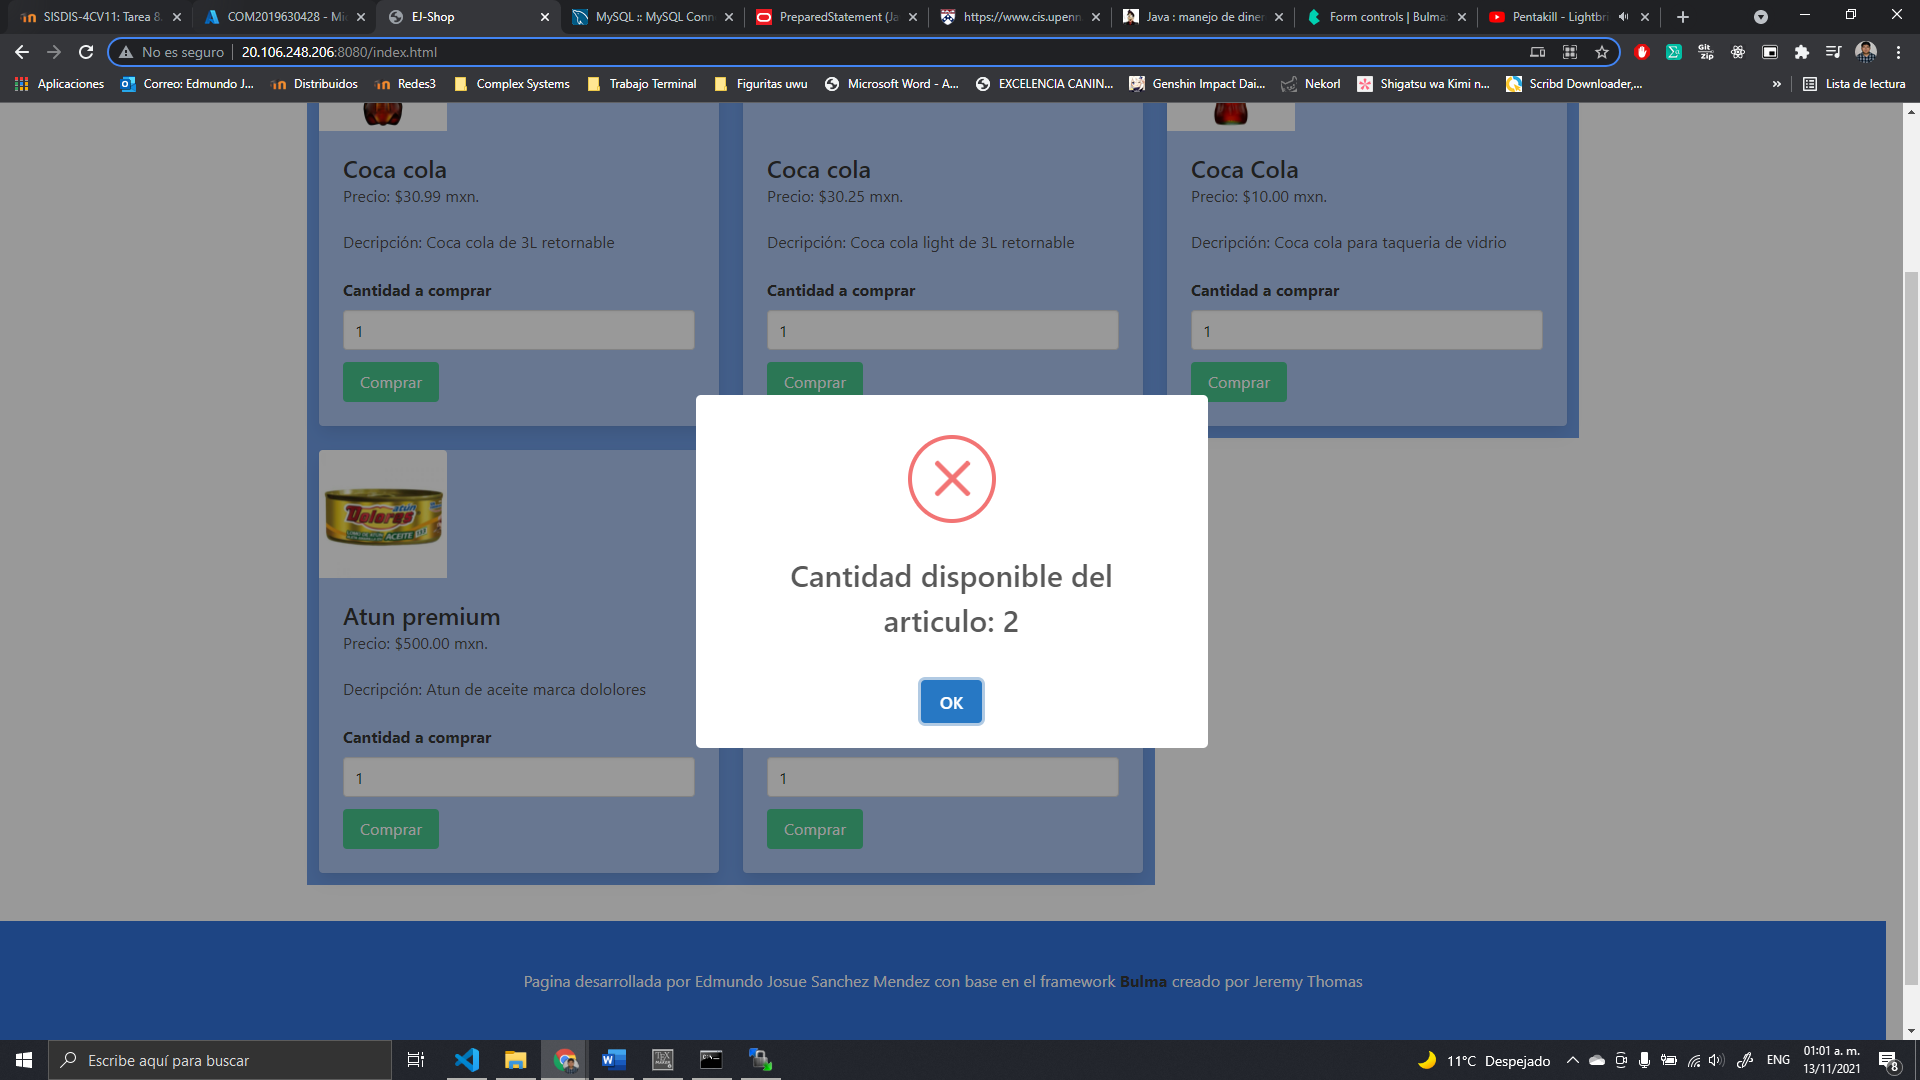
\includegraphics[scale=0.34]{resources/p3mas1.png}
			\caption{Respuesta del sistema.}\label{fig:picture}
		\end{figure}
		\begin{figure}[H]
			\centering
			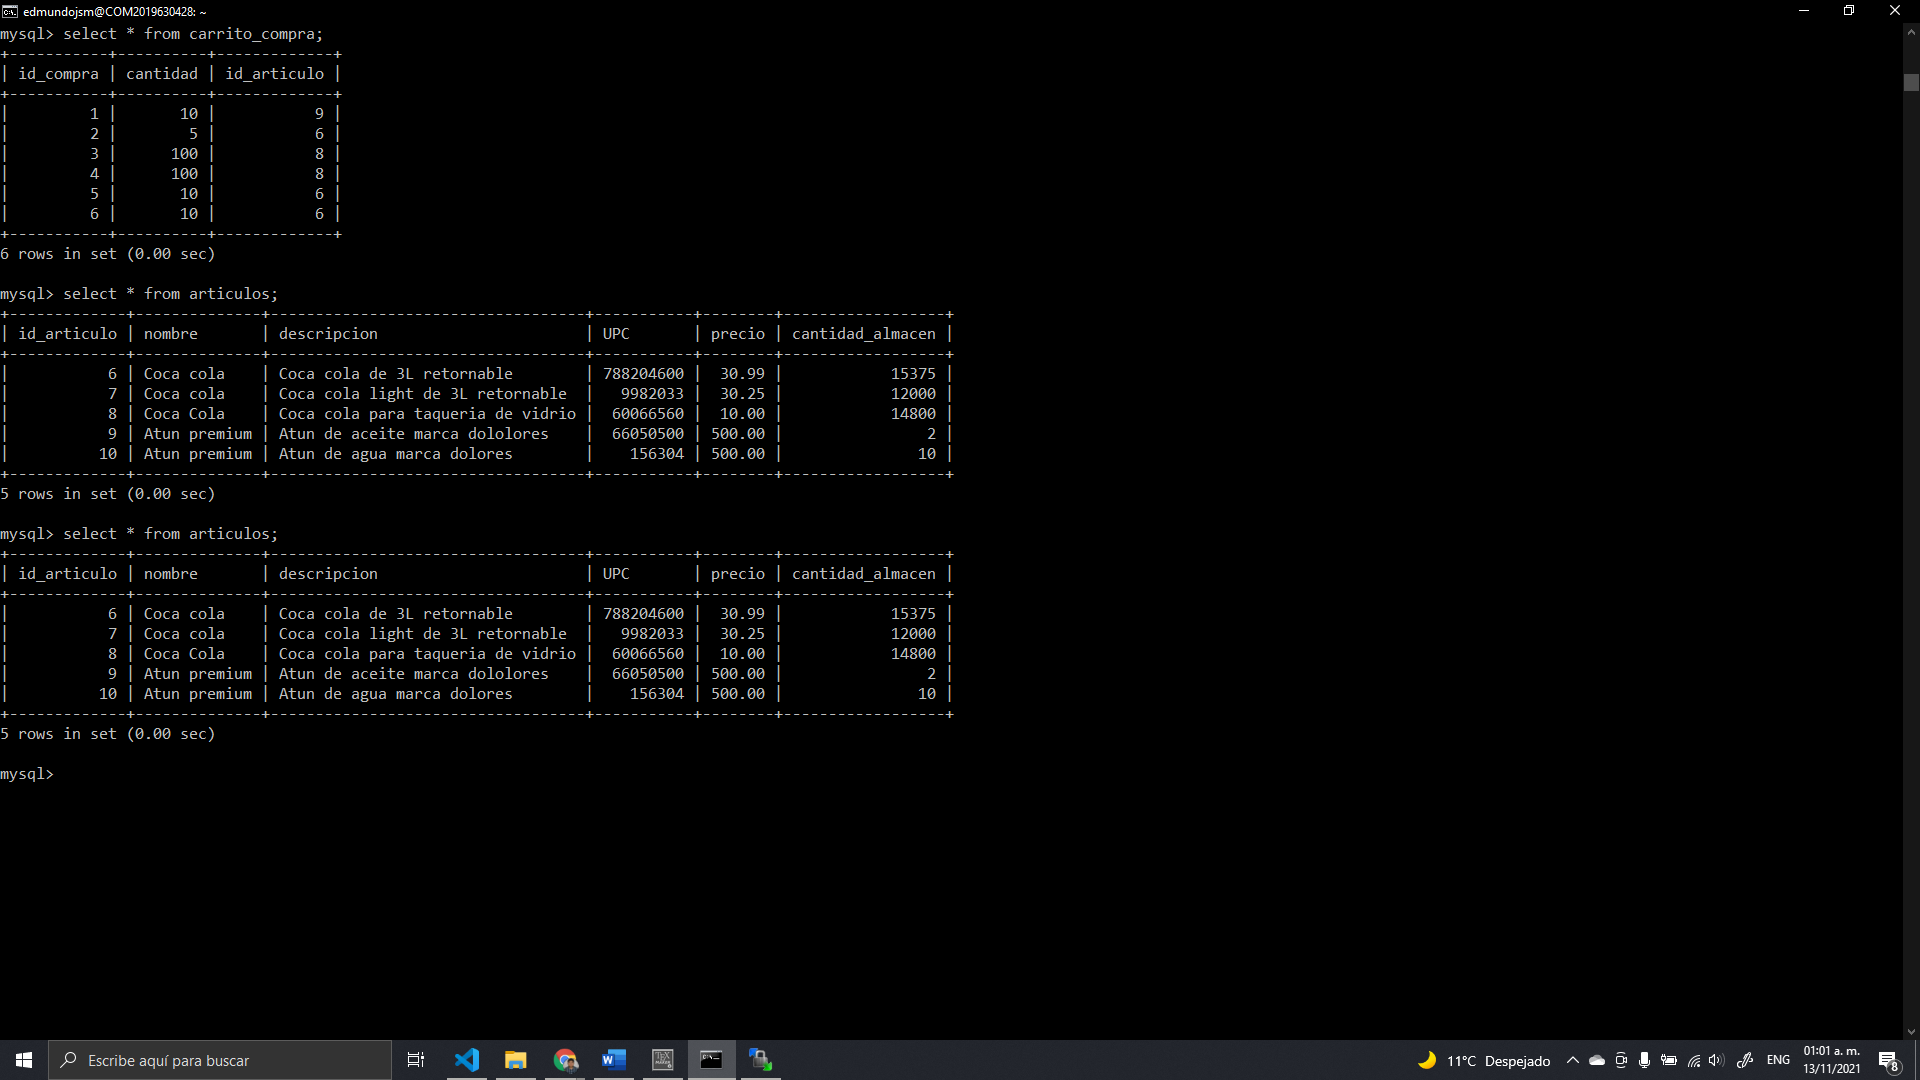
\includegraphics[scale=0.34]{resources/p3masbd.png}
			\caption{Base de datos no modificada.}\label{fig:picture}
		\end{figure}
		Finalmente en las siguientes 3 figuras veamos una vez el intento de compra de la cantidad artículos exacta que están disponibles, como vemos en la base de datos no hay cambio alguno.
		\begin{figure}[H]
			\centering
			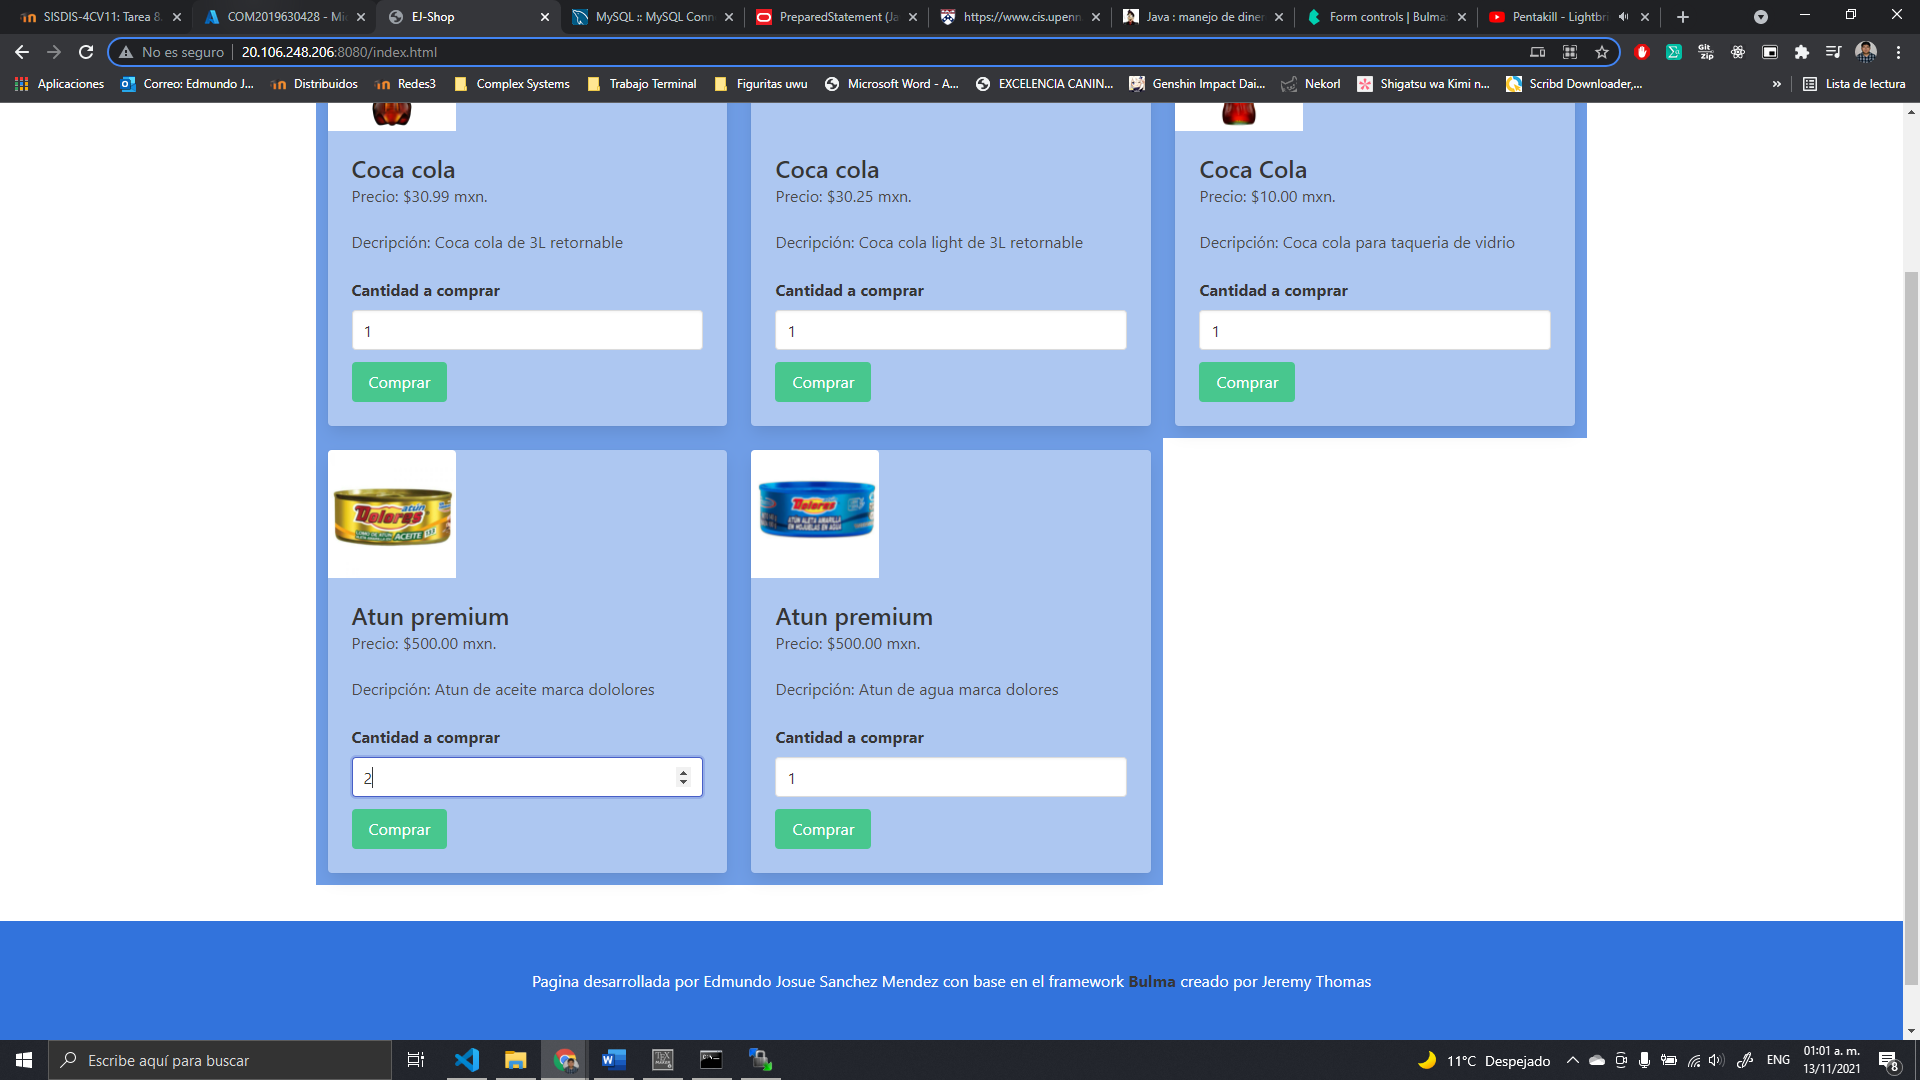
\includegraphics[scale=0.34]{resources/p3mascond.png}
			\caption{Intento de compra de producto exacto.}\label{fig:picture}
		\end{figure}
		\begin{figure}[H]
			\centering
			\includegraphics[scale=0.34]{resources/p3mascon1.png}
			\caption{Respuesta del sistema.}\label{fig:picture}
		\end{figure}
		\begin{figure}[H]
			\centering
			\includegraphics[scale=0.34]{resources/p3masconbd.png}
			\caption{Base de datos modificada y con 0 en cantidad restante.}\label{fig:picture}
		\end{figure}
		\subsection{Prueba 4. Carrito de compra}
	Ahora veamos como se ve el carrito de compra, en las figuras siguientes veremos como se ve el carrito de compras tanto en celular como en celular.
		\begin{figure}[H]
			\centering
			\includegraphics[scale=0.34]{resources/p4.png}
			\caption{Desplegado del carrito de compra en computadora.}\label{fig:picture}
		\end{figure}
		\begin{figure}[H]
			\centering
			\includegraphics[scale=0.27]{resources/Screenshot_20211113-023957.png}
			\caption{Desplegado del carrito de compra en celular.}\label{fig:picture}
		\end{figure}
		\begin{figure}[H]
			\centering
			\includegraphics[scale=0.27]{resources/Screenshot_20211113-024007.png}
			\caption{Desplegado del carrito de compra en celular.}\label{fig:picture}
		\end{figure}
		Finalmente veamos la base de datos resultante del carrito de compra.
		\begin{figure}[H]
			\centering
			\includegraphics[scale=0.34]{resources/p4bd.png}
			\caption{Base de datos con el contenido del carrito de compra.}\label{fig:picture}
		\end{figure}	
		\section{Conclusiones}
	Al igual que en la tarea anterior observamos el funcionamiento de una aplicación REST,ahora esto lo podemos ver como un sistema mas competo y no solo eso y es que lo que se desarrollo es incluso un sistema que se podría vender a la típica tiendita de la esquina para que pueda llevar un control del inventario de forma electrónica y es que en la mayoría de las tiendas de la esquina aun siguen usando papel para llevar el inventariado de lo que venden y no solo lo podemos dejar aquí y es que si se le dedica mas tiempo a esta aplicación estamos hablando de poder desarrollar un e-commerce ya sea para que nosotros vendamos cosas o venderlo para que otras personas lo usen para sus fines personales, sin duda alguna una practica interesante de desarrollar e integradora varias materias que se toman a lo largo de la carrera en ESCOM. Mencionar también que todo lo usado se encontrara en este mismo .zip por si se requiere hacer pruebas del trabajo entregado, también recordar que el script de la base de datos se encuentra disponible en el archivo .txt
		\begin{thebibliography}{1}
 \bibitem[label1]{cite_key1} Dev.mysql.com. 2021. MySQL :: MySQL Connector/J 5.1 Developer Guide :: 5.5 Java, JDBC and MySQL Types. [online] Available at: https://dev.mysql.com/doc/connector-j/5.1/en/connector-j-reference-type-conversions.html [Accessed 13 November 2021].
  \bibitem[label1]{cite_key1} Docs.oracle.com. 2021. PreparedStatement (Java Platform SE 7 ). [online] Available at: https://docs.oracle.com/javase/7/docs/api/java/sql/PreparedStatement.html\#setBigDecimal\par(int,\%20java.math.BigDecimal) [Accessed 13 November 2021].
   \bibitem[label1]{cite_key1} Cis.upenn.edu. 2021. [online] Available at: https://www.cis.upenn.edu/\~{}bcpierce/courses/629/jdkdocs/guide/jdbc/getstart/mapping.doc.html [Accessed 13 November 2021].
     
\end{thebibliography}
\end{document}
